%
%
\documentclass[11pt]{article}
\newcommand{\teilnr}{0}
%
%
\usepackage[margin=1.2in]{geometry}
\usepackage{graphicx}
%
\makeatletter\newcommand*{\captionfigur}{\def\@captype{figure}\caption}\makeatother
\usepackage{tikz}\usetikzlibrary{fit,calc,arrows.meta,backgrounds}   %
%
\renewcommand{\topfraction}{0.85}\renewcommand{\textfraction}{0.1}\renewcommand{\floatpagefraction}{0.75}
\graphicspath{{../abbildungen/}}   %
\usepackage[T1]{fontenc}
\usepackage{lmodern}
\usepackage{amsmath,amssymb,amsthm}
\usepackage{etoolbox}
\usepackage{refcount}
\usepackage{array}       %
\usepackage{longtable}   %
\usepackage[hidelinks]{hyperref}

\providecommand{\teilnr}{?}
\newif\ifimband

%
\newtheorem{theorem}{Theorem}[section]
\newtheorem{proposition}[theorem]{Proposition}
\newtheorem{lemma}[theorem]{Lemma}
\newtheorem{corollary}[theorem]{Corollary}
\theoremstyle{definition}
\newtheorem{definition}[theorem]{Definition}
\theoremstyle{remark}
\newtheorem{remark}[theorem]{Remark}
\newtheorem{question}[theorem]{Question}
\renewcommand{\thetheorem}{\teilnr.\arabic{section}.\arabic{theorem}}
\numberwithin{equation}{section}
%
%
\def\theHtheorem{\teilnr.\arabic{section}.\arabic{theorem}}
\def\theHsection{\teilnr.\arabic{section}}
\def\theHequation{\teilnr.\arabic{section}.\arabic{equation}}

%
%
%
%
\newcommand{\tlabel}[1]{\label{\teilnr:#1}}
%
%
%
\newwrite\belegaus
\immediate\openout\belegaus=\jobname.bel
\newcommand{\belegart}[1]{\immediate\write\belegaus{\thetheorem|#1|\thesection}{\normalfont\small[#1]}\ }
\newcommand{\tref}[1]{\ref{\teilnr:#1}}
\makeatletter
\newcommand{\partref}[2]{%
  \edef\serie@teil{\teilnr}\def\serie@ziel{#1}%
  \ifx\serie@teil\serie@ziel\ref{#1:#2}%
  \else\ifimband\ref{#1:#2}%
  \else\getrefnumber{#1:#2}~in~[Part~#1]\fi\fi}
\makeatother

%
%
%
%
\makeatletter
%
\@namedef{Z@nenner}{811}
%
\@namedef{Z@offen}{6}
%
\@namedef{Z@erledigt}{805}
%
\@namedef{Z@zertifiziert}{767}
%
\@namedef{Z@vollzerlegt}{38}
%
\@namedef{Z@csechsquadrat}{1.3685}
%
\@namedef{Z@csechswalker}{0.3137}
%
\@namedef{Z@csechs}{1.6822}
%
\@namedef{Z@streifenfam}{206}
%
\@namedef{Z@streifentot}{52}
%
\@namedef{Z@streifentuerme}{154}
%
\@namedef{Z@streifenstellen}{8.4\cdot 10^{7}}
%
\@namedef{Z@streifenminm}{223}
%
\@namedef{Z@streifensieben}{17.5}
%
\@namedef{Z@streifeneins}{2}
%
\@namedef{Z@margestich}{530}
%
\@namedef{Z@margemax}{10^{8}}
%
\@namedef{Z@margerand}{2\cdot 10^{5}}
%
\@namedef{Z@margemin}{21.5}
%
\@namedef{Z@streifenschranke}{2000}
%
\@namedef{Z@streifensteckt}{14}
%
\@namedef{Z@glattkerne}{889\,437}
%
\@namedef{Z@glattkand}{0}
%
\@namedef{Z@glattunten}{10^{8}}
%
\@namedef{Z@glattoben}{10^{15}}
%
\@namedef{Z@glatthoehe}{2000}
%
\@namedef{Z@glattprim}{100}
%
\@namedef{Z@glattmin}{4}
%
\@namedef{Z@glattperiode}{9573}
%
\@namedef{Z@glattgross}{356\,888}
%
\@namedef{Z@glattrest}{532\,549}
%
\@namedef{Z@bboxkern}{10^{6}}
%
\@namedef{Z@bboxb}{10^{4}}
%
\@namedef{Z@bboxfam}{101\,329}
%
\@namedef{Z@bboxparitaet}{32\,118}
%
\@namedef{Z@bboxpaare}{421\,010\,513}
%
\@namedef{Z@bboxohnealpha}{343\,504\,538}
%
\@namedef{Z@bboxzweiadisch}{16\,603\,302}
%
\@namedef{Z@bboxkgerade}{11\,242\,224}
%
\@namedef{Z@bboxlemmal}{49\,659\,524}
%
\@namedef{Z@bboxrest}{925}
%
\@namedef{Z@ballotfaelle}{56}
%
\@namedef{Z@ballotgedruckt}{0}
%
\@namedef{Z@ballotfib}{50}
%
\@namedef{Z@turmk1}{1.1\cdot 10^{13}}
%
\@namedef{Z@turmk2}{5.5\cdot 10^{13}}
%
\@namedef{Z@turmk3}{4.5\cdot 10^{30}}
%
\@namedef{Z@turmstellen}{2.5\cdot 10^{15}}
%
\@namedef{Z@kongruenzbis}{10^{5}}
%
\@namedef{Z@kongruenzdichte}{2.67\cdot 10^{-4}}
%
\@namedef{Z@yokoimax}{20000}
%
\@namedef{Z@yokoipaare}{123}
%
\@namedef{Z@designkerne}{251}
%
\@namedef{Z@designtmax}{399}
%
\@namedef{Z@designfenster}{17}
%
\@namedef{Z@designmaxm}{1023}
%
\@namedef{Z@designstellen}{2000}
%
\@namedef{Z@quadratzeuge1}{701}
%
\@namedef{Z@quadratzeuge2}{3}
%
\@namedef{Z@quadratzeuge3}{5}
%
\@namedef{Z@mittenquadrat}{0.3648}
%
\@namedef{Z@mittendoppel}{0.2580}
%
\@namedef{Z@mittensatza}{0.6228}
%
\@namedef{Z@mittenN}{10^{14}}
%
\@namedef{Z@mittengemessen}{0.6252}
%
\@namedef{Z@kerne}{10\,132\,126}
%
\@namedef{Z@kernschranke}{10^{8}}
%
\@namedef{Z@hoehe}{2000}
%
\@namedef{Z@zeugenschranke}{2\cdot 10^{5}}
%
\@namedef{Z@filterfamilien}{83}
%
\@namedef{Z@punktfamilien}{79}
%
\@namedef{Z@punkte}{445}
%
\@namedef{Z@paritaetspunkte}{74}
%
\@namedef{Z@zeugenpunkte}{371}
%
\@namedef{Z@restpunkte}{0}
%
\@namedef{Z@beispielm}{7}
%
\@namedef{Z@beispielk}{7}
%
\@namedef{Z@beispielzeuge}{29}
%
\@namedef{Z@beispielwert}{130\,576\,328}
%
\@namedef{Z@beispielfaktoren}{2^{3}\cdot 29\cdot 197\cdot 2857}
%
\@namedef{Z@ohnetripel}{3.88\cdot 10^{20}}
%
\@namedef{Z@ohnetripelsicher}{1.83\cdot 10^{18}}
%
\@namedef{Z@famtab}{(2, 1) & 1 & 0.90 & 1.53 & 14 \\
(3, 1) & 3 & 2.83 & 3.43 & 6 \\
(23, 2) & 1 & 4.09 & 9.37 & 2 \\
(6, 1) & 3 & 5.37 & 5.97 & 3 \\
(1, 5) & 5 & 5.67 & 12.54 & 2 \\
(46, 1) & 1 & 8.77 & 9.37 & 2 \\
(7, 2) & 7 & 9.73 & 20.67 & 1 \\
(5, 1) & 5 & 11.94 & 12.54 & 1 \\
(430, 1) & 1 & 12.91 & 13.52 & 1 \\
(79, 23) & 1 & 13.08 & 27.36 & 1 \\
(3, 7) & 7 & 13.69 & 28.58 & 1 \\
(10, 1) & 5 & 15.19 & 15.79 & 1 \\
(7, 1) & 7 & 16.23 & 16.83 & 1 \\
(14, 1) & 7 & 20.07 & 20.67 & 1 \\
(1022, 57) & 1 & 20.21 & 41.62 & 1 \\
(19, 35) & 5 & 21.59 & 44.38 & 1 \\}
%
\@namedef{Z@famzahl}{16}
%
\@namedef{Z@famtabzwei}{14}
%
\@namedef{Z@fampaare}{39}
%
\@namedef{Z@famquadrat}{32}
%
\@namedef{Z@famohne}{7}
%
\@namedef{Z@paargrenze}{3.89\cdot 10^{21}}
%
\@namedef{Z@paarletzt}{3\,887\,785\,221\,910\,670\,811\,499}
%
\@namedef{Z@periodepk}{6082}
%
\@namedef{Z@periodepkmax}{10\,000}
%
\@namedef{Z@walkerpk}{955}
%
\@namedef{Z@walkerpkmax}{3000}
%
\@namedef{Z@paare52}{26}
%
\@namedef{Z@paare52exp}{52}
%
\@namedef{Z@mersennemax}{63}
%
\@namedef{Z@famquadratfam}{10}
%
\@namedef{Z@quadratbmax}{10^{4}}
%
\@namedef{Z@walkerdmax}{10^{6}}
%
\@namedef{Z@expfam}{750}
%
\@namedef{Z@expmmax}{10^{4}}
%
\@namedef{Z@exppmax}{3000}
%
\@namedef{Z@exppaare}{120\,373}
%
\@namedef{Z@expwzwei}{470}
%
\@namedef{Z@expwdrei}{52}
%
\@namedef{Z@exphzwei}{486}
%
\@namedef{Z@exphdrei}{49.1}
%
\@namedef{Z@korrs}{411.7}
%
\@namedef{Z@korrmu}{436.2}
%
\@namedef{Z@korrsd}{28.2}
%
\@namedef{Z@korrreps}{4000}
%
\@namedef{Z@korrz}{-0.87}
%
\@namedef{Z@korrp}{0.80}
%
\@namedef{Z@korrvert}{396, 255, 83, 15, 1}
%
\@namedef{Z@korrmaxp}{181}
%
\@namedef{Z@korrmaxz}{2.4}
%
\@namedef{Z@trennvoll}{652}
%
\@namedef{Z@trennzwei}{90}
%
\@namedef{Z@trennfuenf}{48}
%
\@namedef{Z@trennlaeufe}{40}
%
\@namedef{Z@alekterme}{33}
%
\@namedef{Z@alekstellen}{67}
%
\@namedef{Z@klassedreimax}{10^{8}}
%
\@namedef{Z@alekneun}{9}
%
\@namedef{Z@vollexpo}{36}
%
\@namedef{Z@vollmexpo}{24}
%
\@namedef{Z@reinhartt1}{94}
%
\@namedef{Z@reinharttab}{4\,099\,215 & 228 & $2\cdot 10^{5}$ & 701, 100469, 157049 & $1.1\cdot 10^{13}$ & $2.5\cdot 10^{15}$ \\
39\,028\,039\,587\,479 & 1\,880\,030 & $3\cdot 10^{3}$ & 5, 7, 71, 1657; 19, 29, 421, 569, 1987; 379, 2089, 2203, 2437 & $4.5\cdot 10^{30}$ & $8.6\cdot 10^{36}$ \\}
%
\@namedef{Z@reinhartungerade}{209\,991}
%
\@namedef{Z@reinhartungerade2}{117\,477\,414\,815}
%
\@namedef{Z@reinhartboxk}{1, 3, 5, 7}
%
\@namedef{Z@reinhartboxz}{701, 11, 19, 29}
%
\@namedef{Z@reinhartungeradest}{95}
%
\@namedef{Z@reinhartungeradest2}{11\,621}
%
\@namedef{Z@zeugenalle}{371}
%
\@namedef{Z@zeugenprim}{8}
%
\@namedef{Z@zeugenmedian}{19}
%
\@namedef{Z@zeugenmax}{114\,997}
%
\@namedef{Z@zeugen29}{79}
%
\@namedef{Z@zeugen19}{78}
%
\@namedef{Z@zeugen11}{45}
%
\@namedef{Z@zeugen3}{43}
%
\@namedef{Z@zeugen5}{33}
%
\@namedef{Z@zeugen7}{25}
%
\@namedef{Z@zeugennkp}{197}
%
\@namedef{Z@zeugennkk}{1379}
%
\@namedef{Z@zeugennkv}{2}
%
\@namedef{Z@rizzierfuellt}{328}
%
\@namedef{Z@rizzinicht}{43}
%
\@namedef{Z@kongrp}{10^{6}}
%
\@namedef{Z@kongrkerne}{15}
%
\@namedef{Z@kongrpaare}{425\,362}
%
\@namedef{Z@bedpunkte}{445}
%
\@namedef{Z@bedteiler}{2149}
%
\@namedef{Z@bedausweg}{1682}
%
\@namedef{Z@bedanteil}{78.3}
%
\@namedef{Z@bedmedian}{3}
%
\@namedef{Z@bedmittel}{3.8}
%
\@namedef{Z@bedmax}{12}
%
\@namedef{Z@bedallemedian}{4}
%
\@namedef{Z@bedallemax}{16}
%
\@namedef{Z@besp}{3\cdot 10^{6}}
%
\@namedef{Z@beskerne}{25}
%
\@namedef{Z@besnp}{5}
%
\@namedef{Z@bespunkte}{378}
%
\@namedef{Z@besraenge}{2536}
%
\@namedef{Z@besbesetzt}{2025}
%
\@namedef{Z@beszeuge}{1988}
%
\@namedef{Z@beszeugeant}{98.17}
%
\@namedef{Z@beswief}{37}
%
\@namedef{Z@besleer}{511}
%
\@namedef{Z@beseinsnp}{1}
%
\@namedef{Z@beseinszeuge}{1936}
%
\@namedef{Z@beseinsant}{95.60}
%
\@namedef{Z@beseinswief}{89}
%
\@namedef{Z@rgpaare}{961}
%
\@namedef{Z@rgkerne}{79}
%
\@namedef{Z@rgerledigt}{954}
%
\@namedef{Z@rgzert}{954}
%
\@namedef{Z@rgvoll}{0}
%
\@namedef{Z@pbbausteine}{41}
%
\@namedef{Z@pbzahlen}{24}
%
\@namedef{Z@pbpock}{18}
%
\@namedef{Z@pbecpp}{6}
%
\@namedef{Z@pbpockmax}{75}
%
\@namedef{Z@pbecppmax}{477}
%
\@namedef{Z@rgoffen}{7}
%
\@namedef{Z@rgprpzeuge}{0}
%
\@namedef{Z@rgbedingt}{0}
%
\@namedef{Z@teilevollm}{23}
%
\@namedef{Z@teilevolld}{161}
%
\@namedef{Z@teilevolla}{111}
%
\@namedef{Z@teilevollb}{112}
%
\@namedef{Z@teilezeugem}{7}
%
\@namedef{Z@teilezeuged}{1449}
%
\@namedef{Z@teilezeugest}{477}
%
\@namedef{Z@rgaltkerne}{25}
%
\@namedef{Z@rgneukerne}{54}
%
\@namedef{Z@rgungerade}{21}
%
\@namedef{Z@wegetab}{certified witness: search by position, small primes & 605 & 103 & 708 \\
certified witness: search by position, congruence filter & 64 & 16 & 80 \\
certified witness: elliptic curves and $p - 1$ (SymPy) & 70 & 0 & 70 \\
certified witness: elliptic curves (GMP-ECM) & 27 & 20 & 47 \\
certified witness: $M_d$ itself prime, with a certificate & 8 & 8 & 16 \\
certified witness: complete factorization, factors proved prime & 32 & 0 & 32 \\
certified witness: a factor of the algebraic split, proved prime & 1 & 0 & 1 \\
open & 4 & 3 & 7 \\}
%
\@namedef{Z@bouchardn}{9800}
%
\@namedef{Z@bouchardp}{13}
%
\@namedef{Z@bouchardfakt}{2\cdot 13^{2}\cdot 29}
%
\@namedef{Z@pellwief}{13,\ 31,\ 1546463}
%
\@namedef{Z@reinhartza}{701}
%
\@namedef{Z@reinhartzc}{5}
%
\@namedef{Z@offentab}{399 & 171 & 173 & 300 & 1071 & 2753 & 8.36 & 1.10 \\
407 & 111 & 269 & 300 & 1071 & 2753 & 8.36 & 1.10 \\
39 & 247 & 367 & 300 & 1071 & 2753 & 8.36 & 1.10 \\
111 & 185 & 400 & 300 & 1071 & 2753 & 8.36 & 1.10 \\
407 & 259 & 805 & 300 & 1071 & 2753 & 8.05 & 1.05 \\
663 & 663 & 889 & 300 & 1071 & 38 & 1.05 & 0.11 \\
20\,303 & 257 & 1893 & 300 & 209 & -- & 0.22 & 0.02 \\}
%
\@namedef{Z@wfinpop}{3}
%
\@namedef{Z@offenmin}{173}
%
\@namedef{Z@erstesucheP}{3\cdot 10^{6}}
%
\@namedef{Z@siebober}{10^{9}}
%
\@namedef{Z@prtripel}{1341}
%
\@namedef{Z@prvauf1}{1338}
%
\@namedef{Z@prvauf2}{3}
%
\@namedef{Z@prerwartet}{2.38}
%
\@namedef{Z@zweip}{10^{6}}
%
\@namedef{Z@zweiamax}{100\,000}
%
\@namedef{Z@zweiexp}{99\,999}
%
\@namedef{Z@zweiminus}{8957}
%
\@namedef{Z@zweiminusant}{8.96}
%
\@namedef{Z@zweiplus}{2511}
%
\@namedef{Z@zweiplusant}{2.51}
%
\@namedef{Z@zweiminusok}{91\,042}
%
\@namedef{Z@zweiplusok}{97\,488}
%
\@namedef{Z@zweistellen}{30\,103}
%
\@namedef{Z@wfereignisse}{54}
%
\@namedef{Z@wfprimzahlen}{40}
%
\@namedef{Z@wfkerne}{79}
%
\@namedef{Z@wfp}{3\cdot 10^{6}}
%
\@namedef{Z@wfungerade}{18}
%
\@namedef{Z@wfgerade}{15}
%
\@namedef{Z@wfzeuge}{11}
%
\@namedef{Z@wfoffen}{3}
%
\@namedef{Z@wfentschieden}{12}
%
\@namedef{Z@wfmgross}{1\,375\,502\,561}
%
\@namedef{Z@wfmgroesser}{158\,585\,313\,121}
%
\@namedef{Z@wfmquadrat}{20161}
%
\@namedef{Z@erstesuchekerne}{25}
%
\@namedef{Z@lucasgleich}{16}
%
\@namedef{Z@lucaspk}{3}
%
\@namedef{Z@lucasnk}{25}
%
\@namedef{Z@wftab}{15 & 45 & 181 & witness & yes \\
31 & 39 & 157 & witness & no \\
79 & 253 & 4049 & witness & no \\
143 & 13 & 311 & witness & yes \\
223 & 45 & 179 & witness & no \\
319 & 5 & 20\,161 & complete factorization & yes \\
383 & 21545 & 258\,539 & witness & no \\
447 & 413 & 24\,781 & witness & no \\
455 & 9 & 37 & witness & no \\
615 & 807 & 3229 & not settled & no \\
1343 & 5 & 19 & witness & no \\
1535 & 63 & 251 & witness & no \\
2135 & 13 & 53 & witness & no \\
2135 & 37 & 149 & not settled & no \\
123\,879 & 9 & 37 & not settled & no \\}
%
\@namedef{Z@wfinpopzu}{3}
%
\@namedef{Z@wfnullrang}{16}
%
\@namedef{Z@csechsbmax}{10^{6}}
%
\@namedef{Z@csechsfamq}{676\,094}
%
\@namedef{Z@csechsfamw}{275\,371}
%
\@namedef{Z@kdkerne}{10\,132\,121}
%
\@namedef{Z@kdschranke}{10^{8}}
%
\@namedef{Z@kdkandidaten}{86}
%
\@namedef{Z@kdpunkte}{883}
%
\@namedef{Z@kdungerade}{51}
%
\@namedef{Z@kdpaare}{832}
%
\@namedef{Z@kdkernmax}{3\,926\,299}
%
\@namedef{Z@kdpaarkerne}{57}
%
\@namedef{Z@kddrei}{583}
%
\@namedef{Z@kdreinhartst}{99\,134}
%
\@namedef{Z@kdreinhartungst}{117}
%
\@namedef{Z@turmtab}{100 & 14 & 37 & 21 & 67 \\
250 & 39 & 97 & 53 & 168 \\
500 & 83 & 199 & 111 & 344 \\
1000 & 176 & 410 & 224 & 695 \\
1500 & 270 & 616 & 345 & 1049 \\
2000 & 371 & 832 & 467 & 1404 \\}
%
\@namedef{Z@turmc7}{0.1817}
%
\@namedef{Z@turmc3}{0.4134}
%
\@namedef{Z@turmc}{0.595}
%
\@namedef{Z@turmtuerme}{122}
%
\@namedef{Z@turmtuerme7}{60}
%
\@namedef{Z@turmtuerme3}{62}
%
\@namedef{Z@turmueber}{111.8}
%
\@namedef{Z@wtab}{1 & 0.0594 & 0.2914 \\
2 & 0.1341 & 0.3666 \\
3 & 0.1711 & 0.4027 \\
4 & 0.1936 & 0.4212 \\
5 & 0.2047 & 0.4366 \\
6 & 0.2151 & 0.4513 \\
7 & 0.2217 & 0.4566 \\}
%
\@namedef{Z@modellp}{31}
%
\@namedef{Z@modell7min}{0.94}
%
\@namedef{Z@modell7max}{1.01}
%
\@namedef{Z@modell3min}{0.91}
%
\@namedef{Z@modell3max}{1.04}
%
\@namedef{Z@beins7}{87.1}
%
\@namedef{Z@beins3}{86.3}
%
\@namedef{Z@einkernm}{525\,003}
%
\@namedef{Z@einkernanteil}{45}
%
\@namedef{Z@modellc}{0.7482}
%
\@namedef{Z@modellrate}{0.8835}
%
\@namedef{Z@naivrate}{1.1808}
%
\@namedef{Z@modelltab}{8 & 10 & 11.5 & 15.4 \\
10 & 14 & 15.5 & 20.7 \\
12 & 18 & 19.5 & 26.0 \\
14 & 24 & 23.5 & 31.4 \\
16 & 26 & 27.6 & 36.9 \\
18 & 31 & 31.6 & 42.3 \\
20 & 35 & 35.7 & 47.7 \\}
%
\@namedef{Z@modellnull}{39}
%
\@namedef{Z@modellnullkorr}{38.94}
%
\@namedef{Z@modellnullnaiv}{52.04}
%
\@namedef{Z@modellneu}{13}
%
\@namedef{Z@modellneukorr}{12.06}
%
\@namedef{Z@modellneunaiv}{16.12}
%
\@namedef{Z@quadbmax}{10^{4}}
%
\@namedef{Z@quadtab}{49.7 & 32 & 38.9 & 52.0 & 0.7049 \\
75.0 & 54 & 61.3 & 81.9 & 0.7744 \\
100.0 & 76 & 83.4 & 111.4 & 0.8136 \\
150.0 & 124 & 127.5 & 170.4 & 0.8755 \\
200.0 & 171 & 171.7 & 229.5 & 0.9011 \\
300.0 & 265 & 260.1 & 347.6 & 0.9300 \\
500.0 & 468 & 436.8 & 583.7 & 0.9765 \\
1000.0 & 997 & 878.5 & 1174.1 & 1.0345 \\}
%
\@namedef{Z@quadkreuz}{192.9}
%
\@namedef{Z@quadkreuzlog}{83.8}
%
\@namedef{Z@quadgeboren}{103}
%
\@namedef{Z@quadrate1000}{1.0345}
%
\@namedef{Z@quadnq1000}{997}
%
\@namedef{Z@quadv1000}{878.5}
%
\@namedef{Z@quadrest1000}{894}
%
\@namedef{Z@teilsumq1}{0.6055}
%
\@namedef{Z@teilsumq2}{0.8949}
%
\@namedef{Z@teilsumtab}{3 & 1.1044 & 0.1783 & 1.2827 \\
4 & 1.2235 & 0.2385 & 1.4619 \\
5 & 1.3110 & 0.2831 & 1.5941 \\
6 & 1.3685 & 0.3137 & 1.6822 \\}
%
\@namedef{Z@zuwq}{79}
%
\@namedef{Z@zuww}{77}
%
\@namedef{Z@zuwtopq}{71}
%
\@namedef{Z@zuwtopw}{72}
%
\@namedef{Z@a1nmax}{10^{12}}
%
\@namedef{Z@a1dmax25}{10^{5}}
%
\@namedef{Z@a1paare25}{18}
%
\@namedef{Z@a1dmax}{20\,000}
%
\@namedef{Z@a1kerne}{12\,159}
%
\@namedef{Z@a1paare}{6063}
%
\@namedef{Z@a1hoehe}{2000}
%
\@namedef{Z@a1ueber}{7}
%
\@namedef{Z@a1paareh}{6056}
%
\@namedef{Z@a1p1}{5\cdot 10^{5}}
%
\@namedef{Z@a1zeuge1}{4991}
%
\@namedef{Z@a1p2}{5\cdot 10^{6}}
%
\@namedef{Z@a1zeuge2}{154}
%
\@namedef{Z@a1rest2}{918}
%
\@namedef{Z@a1s2prim}{24}
%
\@namedef{Z@a1s2primzert}{5}
%
\@namedef{Z@a1s2ecm}{15}
%
\@namedef{Z@a1s2offen}{879}
%
\@namedef{Z@a1s2kleinst}{81}
%
\@namedef{Z@a1s2probable}{19}
%
\@namedef{Z@a1s2ecpp}{19}
%
\@namedef{Z@a1s2ecppmax}{1687}
%
\@namedef{Z@a1s2nk}{5}
%
\@namedef{Z@quadzeilen}{8}
%
\@namedef{Z@quadab}{300}
%
\@namedef{Z@quadablog}{130}
%
\@namedef{Z@quadslack}{6}
%
\@namedef{Z@wtabmax}{10^{7}}
%
\@namedef{Z@reinhartgerade}{3}
%
\@namedef{Z@reinhartgeradesicher}{1}
%
\@namedef{Z@reinhartsieben}{4}
%
\@namedef{Z@znab}{300}
%
\@namedef{Z@znaq}{183}
%
\@namedef{Z@znaqg}{182}
%
\@namedef{Z@znamit}{34}
%
\@namedef{Z@phidreilavij}{13}
%
\@namedef{Z@phidreibrute}{10^{6}}
%
\@namedef{Z@phidreistellen}{19, 35 and 52}
%
\@namedef{Z@phidreiperiode}{7}
%
\@namedef{Z@zyktab}{3 & 18 & 343 & $7^{3}$ \\
3 & 88\,916 & 7\,906\,143\,973 & $7^{2}\cdot 13^{3}\cdot 271^{2}$ \\
4 & 682 & 465\,125 & $5^{3}\cdot 61^{2}$ \\
5 & 3 & 121 & $11^{2}$ \\
6 & 19 & 343 & $7^{3}$ \\
6 & 88\,917 & 7\,906\,143\,973 & $7^{2}\cdot 13^{3}\cdot 271^{2}$ \\}
%
\@namedef{Z@zykn}{3\,004\,199}
%
\@namedef{Z@zyktreffer}{6}
%
\@namedef{Z@zykschranke}{10^{12}}
%
\@namedef{Z@zykklasse}{10^{14}}
%
\@namedef{Z@lstab}{$10^{12}$ & 2\,158\,391 & 832\,161 & 0.31 & 900 & 69 & 1656 & 183 of 215 \\
$10^{13}$ & 6\,840\,384 & 2\,593\,517 & 0.18 & 44\,100 & 57 & 63\,900 & 189 of 211 \\
$10^{14}$ & 21\,663\,503 & 8\,235\,300 & 0.10 & 44\,100 & 48 & 63\,900 & 191 of 201 \\}
%
\@namedef{Z@lsnpw}{21\,663\,503}
%
\@namedef{Z@lswerte}{8\,235\,300}
%
\@namedef{Z@lsanteil}{0.10}
%
\@namedef{Z@lsbis}{48}
%
\@namedef{Z@lsocc}{112}
%
\@namedef{Z@lserster}{63\,900}
%
\@namedef{Z@lsg100}{103}
%
\@namedef{Z@lsg100pw}{102}
%
\@namedef{Z@lsg200}{201}
%
\@namedef{Z@lsg200pw}{191}
%
\@namedef{Z@lserwartet}{0.05}
%
\@namedef{Z@lsdecke}{63\,900 & 900 & 9 & 112 & 50.9 \\
82\,908 & 1764 & 36--41 & 98 & 49.0 \\
17\,100 & 900 & 9 & 97 & 43.3 \\
23\,324 & 1372 & 170--175 & 96 & 20.8 \\
151\,900 & 4900 & 10--11 & 90 & 45.6 \\
171\,900 & 900 & 9 & 90 & 52.2 \\
7100 & 100 & 357--381 & 89 & 61.8 \\
26\,100 & 900 & 9 & 89 & 37.1 \\
127\,800 & 1800 & 29--31 & 89 & 53.9 \\
215\,100 & 900 & 9 & 89 & 51.7 \\}
%
\@namedef{Z@lsdeckeanz}{10}
%
\@namedef{Z@lsg20}{21}
%
\@namedef{Z@lsanteilpw}{24.2--44.9}
%
\@namedef{Z@lsanteilnpw}{20.8--61.8}
%
\@namedef{Z@nvlmax}{50}
%
\@namedef{Z@nvrel}{1.2}
%
\@namedef{Z@nvsteig}{0.63}
%
\@namedef{Z@lstop1}{44\,100}
%
\@namedef{Z@zmn}{62\,118}
%
\@namedef{Z@zmmin}{20}
%
\@namedef{Z@lsbasiswerte}{62\,118}
%
\@namedef{Z@lsbasismind}{20}
%
\@namedef{Z@lsbasisanteil}{4.81}
%
\@namedef{Z@lsbasiserw}{2.4}
%
\@namedef{Z@fpn}{3531}
%
\@namedef{Z@fpmax}{3\cdot 10^{-16}}
%
\@namedef{Z@zmr2}{0.545}
%
\@namedef{Z@zmr2sd}{0.025}
%
\@namedef{Z@zmroh}{0.306}
%
\@namedef{Z@zmrohsd}{0.005}
%
\@namedef{Z@zmr2log}{0.514}
%
\@namedef{Z@zmr2logsd}{0.016}
%
\@namedef{Z@zmallesep}{0.319}
%
\@namedef{Z@zmallesepsd}{0.012}
%
\@namedef{Z@zmalleroh}{0.307}
%
\@namedef{Z@zmallerohsd}{0.004}
%
\@namedef{Z@zmdeutstufen}{3061}
%
\@namedef{Z@zmdeutkmin}{4}
%
\@namedef{Z@zmkern}{0.012}
%
\@namedef{Z@zmkof}{0.272}
%
\@namedef{Z@zmww}{0.001}
%
\@namedef{Z@zmkerne}{2986}
%
\@namedef{Z@zmkof_n}{9752}
%
\@namedef{Z@zmdecke}{0.864}
%
\@namedef{Z@zmdeutung}{0.425}
%
\@namedef{Z@zmdeutdecke}{0.898}
%
\@namedef{Z@pmstich}{401\,176}
%
\@namedef{Z@pmschritt}{54}
%
\@namedef{Z@pmanteil}{47.69}
%
\@namedef{Z@pmgcd}{4,\ 9,\ 8,\ 16,\ 25,\ 36,\ 27,\ 32}
%
\@namedef{Z@ukerne}{25}
%
\@namedef{Z@up}{2\cdot 10^{6}}
%
\@namedef{Z@upaare}{294\,920}
%
\@namedef{Z@u11}{0}
%
\@namedef{Z@u10}{38}
%
\@namedef{Z@u01}{8}
%
\@namedef{Z@uerw}{0.001}
%
\@namedef{Z@usim}{400}
%
\@namedef{Z@utrenn}{98}
%
\@namedef{Z@utrennnull}{1}
%
\@namedef{Z@ukopie}{3.8}
%
\@namedef{Z@wf3kerne}{25}
%
\@namedef{Z@wf3p}{3\cdot 10^{6}}
%
\@namedef{Z@wfn}{5\,420\,294}
%
\@namedef{Z@wftreffer}{56}
%
\@namedef{Z@wferw}{50.71}
%
\@namedef{Z@wft4b}{593}
%
\@namedef{Z@wft4e}{583.9}
%
\@namedef{Z@wfzmax}{1.37}
%
\@namedef{Z@wfklpmin}{0.014}
%
\@namedef{Z@wfklbon}{0.08}
%
\@namedef{Z@wfklanz}{6}
%
\@namedef{Z@wglags}{20}
%
\@namedef{Z@wgtests}{500}
%
\@namedef{Z@wgueber}{7}
%
\@namedef{Z@wgerw}{5}
%
\@namedef{Z@wgzmax}{3.30}
%
\@namedef{Z@wgpbon}{0.48}
%
\@namedef{Z@wgpk}{21.4}
%
\@namedef{Z@wkpaare}{300}
%
\@namedef{Z@wkzmax}{3.61}
%
\@namedef{Z@wkpbon}{0.09}
%
\@namedef{Z@wkpk}{10.0}
%
\@namedef{Z@achtq}{2384}
%
\@namedef{Z@achtgrenze}{10^{5}}
%
\@namedef{Z@zpn}{163}
%
\@namedef{Z@zpprim}{18}
%
\@namedef{Z@zpdmax}{59}
%
\@namedef{Z@zpab16}{5}
%
\@namedef{Z@offenschwach}{0}
%
\@namedef{Z@offenneum}{399, 663 and 20\,303}
%
\@namedef{Z@zquadkerne}{26}
%
\@namedef{Z@zquadbl}{361}
%
\@namedef{Z@zquadprim}{171}
%
\@namedef{Z@zquadgrenze}{5000}
%
\@namedef{Z@reinhartsiebensicher}{3}
%
%
%
%
%
%
%
%
%
%
%
%
%
%
\makeatother

\newcommand{\Z}[1]{%
  \ifcsname Z@#1\endcsname\csname Z@#1\endcsname
  \else\PackageError{serie}{Zahl '#1' ist nicht in zahlen.tex definiert}{werkzeug/zahlen_bauen.py laufen lassen oder den Schluessel pruefen}\fi}

%
%
%
%
%
\newcommand{\inwords}{\par\medskip\noindent\textit{In words.}\ }
%
\newcommand{\spaeter}[1]{\par\noindent\textit{[#1]}\par}
\newcommand{\PrimSymbol}{M}
\newcommand{\Prim}[1]{\PrimSymbol_{#1}}
\newcommand{\Kreis}[1]{\Phi_{#1}}

\imbandtrue
%
\providecommand{\problemeletzter}{I}\providecommand{\problemeanzahl}{9}
\providecommand{\problemvon}[1]{\ifcsname prob@#1\endcsname\csname prob@#1\endcsname\else\textbf{??}\fi}
\expandafter\def\csname prob@I:q:walsh\endcsname{A}
\expandafter\def\csname prob@I:q:primindex\endcsname{B}
\expandafter\def\csname prob@I:q:zweierpotenz\endcsname{C}
\expandafter\def\csname prob@I:q:reinhart\endcsname{D}
\expandafter\def\csname prob@II:q:konvergenz\endcsname{E}
\expandafter\def\csname prob@II:q:wachstum\endcsname{F}
\expandafter\def\csname prob@II:q:ezwei\endcsname{G}
\expandafter\def\csname prob@III:q:luecken\endcsname{H}
\expandafter\def\csname prob@III:q:phiacht\endcsname{I}

\title{Consecutive Powerful Numbers and Pell Equations: Triples, Pairs, and Further Observations}
\author{Berkay Y\"uksel Sayim\\
Independent Researcher, Germany\\
\texttt{berksa@tutamail.com} $\cdot$ ORCID 0009-0004-4993-7352}
\date{October 4, 2026}
\hypersetup{pdfauthor={Berkay Y\"uksel Sayim}, pdftitle={Consecutive Powerful Numbers and Pell Equations: Triples, Pairs, and Further Observations}}
\begin{document}
\maketitle
\begin{abstract}
%
A positive integer is \emph{powerful} if every prime that divides it divides it at least twice. Pairs of consecutive powerful numbers exist
in abundance, but no three consecutive powerful numbers are known, and Erd\H{o}s asked whether they exist. This volume collects three parts.
Part~I turns a hypothetical triple into an address on a Pell equation, proves a lower bound for its middle in terms of its kernel, and
reduces the existence of a triple to primes that divide a Pell number exactly once. Using Reinhart's complete list of the kernels $m$ up to
$1.5 \cdot 10^{12}$ that divide $U_1(m)$, where $T_1 + U_1\sqrt{m}$ is the smallest solution of $x^2 - m y^2 = 1$ with $y > 0$, it shows by
computation that no triple has a middle below $\Z{ohnetripelsicher}$. Independently of this bound, it asks whether the \Z{rgpaare} building
blocks attached to the lattice points it examines can be powerful: \Z{rgzert} are shown not to be, by witnesses proved prime,
and \Z{rgoffen} remain open. Part~II establishes the
explicit lower bound $\liminf N_1(x)/\log x \ge \Z{csechs}$ for the number $N_1(x)$ of pairs $n, n + 1$ with $n + 1 \le x$, a logarithmic
lower bound at distance two, and shows that the number of pairs at distance two up to $x$ differs by $O(x^{2/9})$ from the number of
kernels $m$ with $m \mid U_1(m)$, $T_1(m)$ even and $T_1(m) \le x$. Part~III collects
the gap spectrum of powerful numbers, powerful values of cyclotomic polynomials, and tests of the independence assumptions behind the
heuristic, each with the power of the test. Every computed number is generated from deposited data or from a cited constant, every numbered statement is labeled by
the kind of evidence behind it, and the open questions are collected as Problems~A to~\problemeletzter.
\end{abstract}
%
\paragraph{About this series.}
\ifimband This volume collects three parts that share\else This paper is one of three parts that share\fi\ one source, one bibliography, and one numbering.
A statement numbered I.4.5 carries that number in its part and in the collected volume.
Every number that we computed is generated from the result files of the data deposit or from a cited constant; numbers from the literature carry a citation. The ranges and parameters of a computation and the constants of an argument are written in the text.
The open questions of all parts are collected as Problems~A to~\problemeletzter\ \ifimband in the framework introduction below\else in the framework
introduction of the collected volume\fi\ and in the file \texttt{OPEN\_PROBLEMS.md} of the data deposit; both are generated from the parts.
This \ifimband volume\else part\fi\ is a preprint. The author corrects any error that becomes visible after the release in a new version of the record; earlier versions remain available under their own version numbers.
%
%
%
%
%
\definecolor{skI}{HTML}{0072B2}\definecolor{skII}{HTML}{D55E00}\definecolor{skIII}{HTML}{009E73}\definecolor{skgrau}{HTML}{5F6368}
\tikzset{sk/duenn/.style={line width=0.5pt}, sk/dick/.style={line width=1.8pt}}
\ifnum\pdfstrcmp{\teilnr}{I}=0 \tikzset{sk/I/.style={sk/dick}}\else\tikzset{sk/I/.style={sk/duenn}}\fi
\ifnum\pdfstrcmp{\teilnr}{II}=0 \tikzset{sk/II/.style={sk/dick}}\else\tikzset{sk/II/.style={sk/duenn}}\fi
\ifnum\pdfstrcmp{\teilnr}{III}=0 \tikzset{sk/III/.style={sk/dick}}\else\tikzset{sk/III/.style={sk/duenn}}\fi
\ifnum\pdfstrcmp{\teilnr}{0}=0 \tikzset{sk/band/.style={sk/dick}}\else\tikzset{sk/band/.style={sk/duenn}}\fi
\providecommand{\skp}[1]{\par\hangindent=0.75em\hangafter=1\noindent\makebox[0.75em][l]{\textbullet}#1}
%
\providecommand{\skspalte}[1]{\parbox[t][4.8cm][t]{4.5cm}{\raggedright\hyphenpenalty=10000\exhyphenpenalty=10000 #1}}
\providecommand{\skdies}[1]{\ifnum\pdfstrcmp{\teilnr}{#1}=0 \\[1pt]\textbf{this document}\fi}
%
%
\par\medskip\noindent\begin{minipage}{\textwidth}
\centering
\begin{tikzpicture}[font=\footnotesize,
  spalte/.style={rectangle, rounded corners=2pt, inner sep=5pt, anchor=north west},
  einzel/.style={rectangle, rounded corners=2pt, align=center, text width=4.0cm, inner sep=4pt, minimum height=0.95cm, anchor=north,
    execute at begin node={\hyphenpenalty=10000\exhyphenpenalty=10000}},
  pfeil/.style={-{Stealth[length=2mm]}, draw=skgrau, line width=0.5pt},
  quer/.style={{Stealth[length=1.6mm]}-{Stealth[length=1.6mm]}, draw=skgrau, line width=0.5pt, dashed}]
\node[spalte, draw=skI, fill=skI!5] (sI) at (0, 0) {\skspalte{\textbf{\color{skI}Part I: triples}\par\smallskip
  {\color{skgrau}Can $n - 1$, $n$, $n + 1$ all be powerful? (Erd\H{o}s)}\par\smallskip
  \skp{the middle is a Pell number $T_k(m)$ at a point $(m, k)$}
  \skp{a height inequality, two wings of kernels}
  \skp{witnesses: primes dividing $T_k$ exactly once}
  \skp{no triple with a middle below $\Z{ohnetripelsicher}$}
  \skp{\Z{rgpaare} building blocks, \Z{rgoffen} open}\par}};
\node[spalte, draw=skII, fill=skII!5] (sII) at (5.05, 0) {\skspalte{\textbf{\color{skII}Part II: pairs}\par\smallskip
  {\color{skgrau}How often are $n$ and $n + 1$ both powerful? (Erd\H{o}s)}\par\smallskip
  \skp{Walker's families; all pairs up to $2^{\Z{paare52exp}}$}
  \skp{$\liminf N_1(x)/\log x \ge \Z{csechs}$}
  \skp{distance two: a sum over towers, a lower bound at every height}
  \skp{upper bounds reduce to the kernels with $m \mid U_1(m)$}\par}};
\node[spalte, draw=skIII, fill=skIII!5] (sIII) at (10.1, 0) {\skspalte{\textbf{\color{skIII}Part III: observations}\par\smallskip
  {\color{skgrau}What else did the study of triples and pairs show?}\par\smallskip
  \skp{the gaps between consecutive powerful numbers}
  \skp{powerful values of cyclotomic polynomials}
  \skp{tests of the independence assumptions, with their power}\par}};
\path let \p1 = (sI.south), \p2 = (sII.south), \p3 = (sIII.south) in
  node[rectangle, rounded corners=2pt, draw=skgrau, fill=skgrau!6, align=center, text width=14.67cm, inner sep=4pt, anchor=north west]
  (rahmen) at (0pt, {min(\y1, \y2, \y3) - 6pt}) {\mbox{framework introduction} \enspace$\cdot$\enspace \mbox{results at a glance} \enspace$\cdot$\enspace
  \mbox{known open problems} \enspace$\cdot$\enspace \mbox{Problems A to \problemeletzter} \enspace$\cdot$\enspace \mbox{data and code availability}};
\node[anchor=south west, font=\footnotesize\bfseries, inner sep=1pt] (bandkopf) at (0, 0.12) {The collected volume};
\begin{scope}[on background layer]
\node[rectangle, rounded corners=4pt, draw=black, sk/band, fit=(sI)(sII)(sIII)(rahmen)(bandkopf), inner sep=6pt] (band) {};
\end{scope}
\node[einzel, draw=skI, fill=skI!5, sk/I] (eI) at ($(sI.north |- band.south) + (0, -0.75)$) {\textbf{\color{skI}Part I} as a paper of its own\skdies{I}};
\node[einzel, draw=skII, fill=skII!5, sk/II] (eII) at ($(sII.north |- band.south) + (0, -0.75)$) {\textbf{\color{skII}Part II} as a paper of its own\skdies{II}};
\node[einzel, draw=skIII, fill=skIII!5, sk/III] (eIII) at ($(sIII.north |- band.south) + (0, -0.75)$) {\textbf{\color{skIII}Part III} as a paper of its own\skdies{III}};
\foreach \x in {I, II, III} \draw[pfeil] (s\x.south |- band.south) -- (e\x.north);
\draw[quer] (eI.east) -- (eII.west);
\draw[quer] (eII.east) -- (eIII.west);
\path let \p1 = (eI.south), \p2 = (eII.south), \p3 = (eIII.south) in
  node[font=\scriptsize, text=skgrau, anchor=north, text width=13.5cm, align=center] at ($(eII.south |- 0pt, {min(\y1, \y2, \y3)}) + (0, -0.08)$)
  {each part also stands as a paper of its own, with the same text and numbering; dashed: the parts refer to each other};
\ifnum\pdfstrcmp{\teilnr}{0}=0 \node[font=\scriptsize\bfseries, anchor=south east, inner sep=1pt] at (band.north east) {this document};\fi
\end{tikzpicture}
\captionfigur{\textbf{What this research did.} It followed two questions of Erd\H{o}s on consecutive powerful numbers, on triples and on pairs,
through Pell equations, proved or computed what it could reach, and recorded the rest as observations and open problems. The collected volume
contains the three parts and the framework that ties them together; each part also stands as a paper of its own, with the same text and numbering,
and the parts refer to each other. The heavier frame marks the document in hand.}
\end{minipage}\par\medskip
   %

\tableofcontents
\clearpage
%
%
\section*{Framework introduction}\addcontentsline{toc}{section}{Framework introduction}

A positive integer is \emph{powerful} if every prime that divides it divides it at least twice. Two consecutive integers can both be
powerful, as $8, 9$ shows, and there are infinitely many such pairs. No three consecutive powerful numbers are known. We expect that there
are none; the introduction of Part~I gives the reasons, and none of them is a proof. This volume collects three parts on these two
situations.

\emph{Part~I} concerns triples $n - 1, n, n + 1$. It translates the middle $n$ into an address $(m, k)$ on a Pell equation, bounds $n$ from
below in terms of the kernel $m$, and profiles a counterexample: where it would have to live, and which kernels are the weak point of the
bound. \emph{Part~II} concerns pairs $n, n + 1$. It enumerates the pairs by families, gives an explicit lower bound for their count, compares
the count with a heuristic yardstick, and localizes the count of pairs at distance two in the kernels that Part~I singles out, together
with their counterparts of the other residue class.
\emph{Part~III} collects further observations: the gaps between consecutive powerful numbers, powerful values of cyclotomic polynomials,
and two tests of the independence assumptions behind the heuristic of Part~I, each with the power of the test.

\emph{How to read the volume.} The parts follow one arc. Part~I states the question and its address system, shows what can be excluded
and why the rest depends on witnesses, and names the step at which the methods stop; a certified witness is found for \Z{rgzert} of the
\Z{rgpaare} building blocks of its finite record. Part~II turns the two halves of a triple into pairs and asks how many there are: towers,
families, an explicit lower bound, and why local models mislead. Part~III collects what we saw around the problem: the gap spectrum,
cyclotomic values, measured independence, and negative results with their reach. The open problems at the end of this introduction are
what remains.

The parts share one source and one numbering: a statement numbered I.4.5 carries that number here and in Part~I. Every numbered
statement carries a label that says what kind of evidence stands behind it (proved, literature, computed, measured, heuristic, open); the
table at the end of each part lists them. A statement that combines several kinds carries the label of the part that needs the most trust: a proof that uses our own computation is labeled computed, and a proof that uses a published result is labeled proved. Every number that we computed is generated from the deposited data files or from a cited
constant; the build refuses a
number that has no source.

The author is an independent researcher who likes numbers and science, not a number theorist or mathematician by training. The series
therefore keeps every claim as narrow as its proof or computation allows and says plainly where, to our knowledge, a question remains
open. It grew out of about two months of research. Specialists are welcome to extend, correct, or cite this work; the author intends it to
help this field progress and hopes that a number theorist will take the next steps.
The question whether three consecutive powerful numbers exist can be settled in only two ways: a triple is found, or a general statement is found that holds at all of the infinitely many addresses at once. Such a statement would have to agree with all results in this field, the formulas and laws of this volume and of the literature, and those still to be found. It need not be a single law: it could also be one exclusion that covers all addresses, or many exclusions that together cover them, in the way that the exclusions for cube middles \cite{Chan2025,She2025,Sayim2026EMW} each cover a part. We do not know yet whether such a statement exists.

\section*{Results at a glance}\addcontentsline{toc}{section}{Results at a glance}

The table lists every statement of our own in each part, grouped by the type of evidence behind it, with the main statements in bold.
Statements taken from the literature are not listed here; the complete list of the statements of a part, with the type of each, stands at the
end of that part. The open questions are listed completely in the section on the open problems below.

\begingroup\small
\begin{longtable}{l l p{8.0cm}}
\hline
part & type & statements \\
\hline
\endhead
Part I (triples) & proved & \textbf{I.2.1~height inequality}\newline \textbf{I.2.4~two wings}\newline \textbf{I.4.6~reduction to a witness statement}\newline \textbf{I.4.8~the divisor count of the Wieferich conditions}\newline \textbf{I.6.10~Wieferich primes of the unit and the primitive parts}\newline \emph{also:} I.2.2~the constant in the height bound; I.2.3~kernel bound; I.3.2~weaker bounds with less work; I.4.3~valuation identity; I.4.4~exponent-3 condition; I.4.7~the $T_1$-part of a lattice point; I.4.10~what the witness condition does not follow from; I.4.11~where a witness in an outer number can sit; I.4.12~two elementary constraints, and the size of the gap; I.4.13~the cyclotomic axis \\
 & computed & \textbf{I.3.1~reduction}\newline \textbf{I.4.5~the $b$-box}\newline \textbf{I.5.1~the strip}\newline \textbf{I.5.3~smooth kernels}\newline \textbf{I.5.4~square-type middles}\newline \textbf{I.6.2~no triple below $\Z{ohnetripelsicher}$, and the pairs at distance two with middle divisible by four}\newline \textbf{I.6.8~the primitive part over an explicit finite set}\newline \textbf{I.6.13~a second primitive prime factor}\newline \textbf{I.7.1~profile}\newline \emph{also:} I.5.5~the share of the candidates covered; I.6.3~ladders for the known kernels dividing $U_1$; I.6.4~the smallest witnesses; I.6.5~the condition modulo $36$ and the witnesses; I.6.6~how many conditions there are, and how often they are met; I.6.7~middles that are powers of two; I.6.11~the Wieferich events of the units; I.6.12~Lucas--Wieferich primes; I.8.2~Yokoi's representation; I.8.3~small units \\
 & measured & \textbf{I.6.1~exponents at the rank} \\
 & open & \emph{finiteness of the kernels of wing (ii)} (Problem~\problemvon{I:q:walsh}); \emph{the primitive part of $T_d(m)$} (Problem~\problemvon{I:q:primindex}); \emph{a middle that is a power of $2$} (Problem~\problemvon{I:q:zweierpotenz}); \emph{Reinhart's condition (C)} (Problem~\problemvon{I:q:reinhart}) \\
\hline
Part II (pairs) & proved & \textbf{II.6.2~the count is a sum over towers}\newline \textbf{II.6.4~localization of the pair count}\newline \textbf{II.6.6~where Tao's argument is weakest}\newline \emph{also:} II.2.1~powerful numbers; II.6.5~what the localization says, and what it does not say; II.7.1~pairs on one Pell equation \\
 & computed & \textbf{II.3.1~the known pairs}\newline \textbf{II.4.1~explicit lower bound}\newline \textbf{II.5.2~the families with a square overtake the comparison function}\newline \textbf{II.6.1~the middles that are not divisible by four}\newline \textbf{II.6.3~lower bound at every height}\newline \textbf{II.7.2~the third number}\newline \emph{also:} II.3.2~completeness inside the families \\
 & heuristic & \textbf{II.5.1~comparison function} \\
 & open & \emph{convergence of the rates} (Problem~\problemvon{II:q:konvergenz}); \emph{growth of the tower rate} (Problem~\problemvon{II:q:wachstum}); \emph{the kernels that divide $U_1$} (Problem~\problemvon{II:q:ezwei}) \\
\hline
Part III (further observations) & proved & \textbf{III.2.2~two explicit chains of powerful values of $\Kreis{3}$ and $\Kreis{6}$}\newline \textbf{III.2.5~the simplest case of $\Kreis{8}$} \\
 & computed & \textbf{III.1.2~the head of the gap spectrum}\newline \textbf{III.2.3~powerful values up to a bound}\newline \emph{also:} III.1.3~a ceiling for common divisors; III.2.1~the values $x^2 + 1$; III.2.4~a class without squares \\
 & measured & \textbf{III.1.4~a counting model, measured}\newline \textbf{III.3.1~no joint event along the divisors, and the power of the test}\newline \textbf{III.4.1~no deviation from equidistribution, memory or coupling}\newline \emph{also:} III.1.5~common factors of pairs \\
 & heuristic & III.5.3~a conjecture on the most frequent gap \\
 & open & \emph{the most frequent gap} (Problem~\problemvon{III:q:luecken}); \emph{powerful values of $x^4 + 1$} (Problem~\problemvon{III:q:phiacht}) \\
\hline
\end{longtable}
\endgroup


\inwords A proved statement stands on a proof in the text, which may use cited results. A computed statement stands on a computation whose data are in the deposit; where it depends on a published search, the statement says so.
A measured statement describes a finite range and claims nothing beyond it, and a heuristic is a yardstick, not a claim.

\section*{Where this work meets known open problems}\addcontentsline{toc}{section}{Where this work meets known open problems}

The questions of this volume touch several known open problems. The table names each one, says what this volume reaches toward it,
and says what stays open. None of these problems is solved here.

\begingroup\small\renewcommand{\arraystretch}{1.25}
\begin{longtable}{>{\raggedright\arraybackslash}p{3.4cm} >{\raggedright\arraybackslash}p{6.9cm} >{\raggedright\arraybackslash}p{3.0cm}}
\hline
problem & what this volume reaches & what stays open \\
\hline
\endhead
Three consecutive powerful numbers (Erd\H{o}s; in a form about Pell numbers, Mollin and Walsh \cite[p.~111]{MollinWalsh1986a}) &
no triple has a middle below $\Z{ohnetripelsicher}$ (Proposition~\ref{I:prop:paarliste}(d); Table~\ref{tab:schranken} compares it with the
bounds in the literature, among them a machine-checked proof below $10^{14}$ \cite{MianSiddique2026}); every lattice point with kernel up to
$\Z{kernschranke}$ and middle below $10^{\Z{hoehe}}$ is excluded (Theorem~\ref{I:thm:reduktion}); the profile of a counterexample
(Theorem~\ref{I:thm:profil}) &
the question itself; Problems~\problemvon{I:q:walsh} to~\problemvon{I:q:reinhart} \\
Wieferich primes of Pell units (for primes that have a rank, the Lucas--Wieferich primes of McIntosh and Roettger \cite{McIntoshRoettger2007}) &
if the unit of a kernel has only finitely many Wieferich primes of odd rank, then all but finitely many of its building blocks are not
powerful (Proposition~\ref{I:prop:lucaswieferich}); below $\Z{wfp}$ the \Z{wfkerne} units of Proposition~\ref{I:prop:raenge} carry
\Z{wfereignisse} Wieferich events, \Z{wfungerade} of them of odd rank $d \ge 5$ (Remark~\ref{I:rem:wfdaten}) &
whether there are only finitely many; Problem~\problemvon{I:q:primindex} \\
Kernels $m$ with $m \mid U_1(m)$ (Walsh's question \cite[p.~97]{Walsh1988}) &
they are the weak point of the height bound (Corollary~\ref{I:cor:fluegel}); Reinhart's list of them is complete up to $1.5 \cdot 10^{12}$
\cite[Remark~5.5]{Reinhart2023}, and for the two known kernels $m \equiv 7 \pmod 8$ with $T_1$ even a ladder shows how large a middle would have to be
(Proposition~\ref{I:prop:reinhart}); the count of pairs at distance two is localized in them (Proposition~\ref{II:prop:lokalisierung}) &
finiteness, Problem~\problemvon{I:q:walsh}; a bound for $E_3$, Problem~\problemvon{II:q:ezwei} \\
The $abc$ conjecture &
an $abc$ inequality with exponent below $4/3$ would exclude all large triples; the exponents derived from the explicit form of the
conjecture are larger, and that form gives only a conditional bound on the middle (Remark~\ref{I:rem:abc}) &
an unconditional route \\
Primitive parts of Lucas sequences (after the primitive divisor theorems of Carmichael \cite{Carmichael1913} and of Bilu, Hanrot and Voutier \cite{BiluHanrotVoutier2001}) &
every divisor $d \ge 5$ of an odd index gives a prime of rank $d$, and every such prime satisfies $p \equiv \pm 1 \pmod{4d}$
(Corollary~\ref{I:cor:teiler}); on \Z{zquadkerne} of the \Z{rgkerne} kernels every building block has at least two distinct prime factors
(Remark~\ref{I:rem:zweiprimitive}) &
whether a building block can be powerful; Problem~\problemvon{I:q:primindex} \\
How many pairs there are (upper bounds at distance two by Chan \cite{Chan2012}, Blomer and Sch{\"o}bel \cite{BlomerSchoebel2013}, and
Tao \cite{Tao2026}) &
an explicit lower bound $\liminf N_1(x)/\log x \ge \Z{csechs}$ at distance one (Proposition~\ref{II:prop:csechs}); at distance two
a bound $N^{\theta}$ for the number of kernels with $m \mid U_1(m)$ and $T_1(m)$ even gives the bound $N^{\max(2/9, \theta)}$ for all
pairs, since the two counts differ by $O(N^{2/9})$ (Proposition~\ref{II:prop:lokalisierung}), and under a squarefreeness assumption the case in which Tao's argument is weakest lies
among those kernels (Remark~\ref{II:rem:tao}) &
the true growth; Problems~\problemvon{II:q:konvergenz}, \problemvon{II:q:wachstum} and~\problemvon{II:q:ezwei} \\
Powerful values of polynomials (De Koninck, Doyon and Luca \cite{DeKoninckDoyonLuca2011}) &
two explicit infinite chains, each giving powerful values of both $x^2 + x + 1$ and $x^2 - x + 1$ (Proposition~\ref{III:prop:phidrei});
one of them contains the prime $x$ reported by Lavi \cite{Lavi2026}; $x^4 + 1 = q^3 a^2$ has no solution for primes $q < 2 \cdot 10^{11}$
(Proposition~\ref{III:prop:phiacht}, by a theorem of Cohn \cite{Cohn1997b} and the published verification of the Ankeny--Artin--Chowla
conjecture \cite{vanderPoortenteRieleWilliams2001,vanderPoortenteRieleWilliams2003}) &
whether $x^4 + 1$ is ever powerful; Problem~\problemvon{III:q:phiacht} \\
Katz's conjecture on Wieferich fractions \cite{Katz2015} &
on \Z{wf3kerne} units and the primes below $\Z{wf3p}$ the Wieferich fractions show no deviation from equidistribution in our measurement, which states its power
(Remark~\ref{III:rem:wieferichbrueche}) &
the conjecture itself \\
\hline
\end{longtable}
\endgroup

\section*{The open problems}\addcontentsline{toc}{section}{The open problems}

The parts end with questions. We collect them here with letters, in the order of the parts, in the wording of the parts. The discussion of
each question, that is, what is known and what an answer would give, stands behind the question in its part. The same list, generated from
the same source, is the file \texttt{OPEN\_PROBLEMS.md} of the data deposit. Erd\H{o}s's own questions, whether a triple exists and whether
$N_1(x)$ is bounded by a power of $\log x$, are not repeated; they are the questions the parts start from.

%
\paragraph{Notation used in the problems.}
\begin{itemize}
\item A positive integer is \emph{powerful} if every prime that divides it divides it at least twice.
\item For a squarefree $m \ge 2$, $\varepsilon_m = T_1 + U_1 \sqrt{m}$ is the fundamental solution of $x^2 - m y^2 = 1$, and $\varepsilon_m^k = T_k + U_k \sqrt{m}$; $T_k(m)$, $U_k(m)$ name the kernel $m$. $m'$ is the product of the primes of $m$ that do not divide $U_1$.
\item The \emph{rank} $\alpha_m(p)$ of a prime $p \nmid m$ is the smallest $k$ with $p \mid T_k(m)$; $M_d$ is the part of $T_d(m)$ supported on the primes of rank exactly $d$ (the \emph{primitive part}).
\item \emph{Wing (ii)} of Part I: the kernels $m \equiv 7 \pmod 8$ with $m \mid U_1(m)$; they are the weak point of the lower bound for a triple.
\item In Part II, the \emph{families} are Walker's Pell families of pairs $n, n + 1$, $F_f$ is the growth factor from one pair of the family $f$ to the next, $w(m) = 1/(2m' \log_{10} \varepsilon_m)$ is the rate of the tower of the kernel $m$, $P_2(N)$ counts the pairs $n - 1, n + 1$ of powerful numbers with $n \le N$, and $E_3(N)$ counts the odd squarefree $m$ with $m \mid U_1(m)$, $T_1(m)$ even and $T_1(m) \le N$.
\item Reinhart's condition (C) is Definition 1.4 of \cite{Reinhart2024}.
\end{itemize}
\par\medskip\noindent\textbf{Problem A} (finiteness of the kernels of wing (ii); Question~\ref{I:q:walsh} in Part~I).\enspace Are there only finitely many squarefree $m \equiv 7 \pmod 8$ with $m \mid U_1(m)$ and $T_1(m)$ even?
\par\medskip\noindent\textbf{Problem B} (the primitive part of $T_d(m)$; Question~\ref{I:q:primindex} in Part~I).\enspace Let $m \equiv 7 \pmod 8$ be squarefree with $T_1(m)$ even, let $d \ge 5$ be odd, and let $\Prim{d}$ be the part of $T_d(m)$ supported on the primes of rank exactly $d$. Can $\Prim{d}$ be powerful?
\par\medskip\noindent\textbf{Problem C} (a middle that is a power of $2$; Question~\ref{I:q:zweierpotenz} in Part~I).\enspace Can $2^a - 1$ and $2^a + 1$ both be powerful for some $a \ge 2$?
\par\medskip\noindent\textbf{Problem D} (Reinhart's condition (C); Question~\ref{I:q:reinhart} in Part~I).\enspace Does Reinhart's condition~(C) \cite[Definition~1.4]{Reinhart2024} hold for some squarefree $d$, that is, is there an index $k$ with $T_k(d)$ powerful and $d \mid U_k(d)$? For $d \mid U_1(d)$ the second condition holds for every $k$.
\par\medskip\noindent\textbf{Problem E} (convergence of the rates; Question~\ref{II:q:konvergenz} in Part~II).\enspace Does $\sum_f 1/\log F_f$, taken over all families, converge?
\par\medskip\noindent\textbf{Problem F} (growth of the tower rate; Question~\ref{II:q:wachstum} in Part~II).\enspace Does $c_M = \sum_{m \le M} w(m)$, the sum over odd squarefree $m$ with $T_1(m)$ even of $w(m) = 1/(2m' \log_{10} \varepsilon_m)$, stay bounded as $M \to \infty$?
\par\medskip\noindent\textbf{Problem G} (the kernels that divide $U_1$; Question~\ref{II:q:ezwei} in Part~II).\enspace Is there a $\theta < 61/180$ with $E_3(N) \ll N^{\theta}$? Since $E_3(N) \le P_2(N)$, Blomer and Sch{\"o}bel give $E_3(N) \ll N^{\gamma}$ for every $\gamma > 61/180$ \cite[Theorem~3]{BlomerSchoebel2013}; the question is whether the squarefree odd $m$ with $m \mid U_1(m)$, $T_1(m)$ even and $T_1(m) \le N$ are rarer than that.
\par\medskip\noindent\textbf{Problem H} (the most frequent gap; Question~\ref{III:q:luecken} in Part~III).\enspace Let $g(x)$ be the most frequent gap between consecutive powerful numbers up to $x$. Is $g(x)$ powerful for all large $x$, and does the share of powerful values among the $N$ most frequent gaps up to $x$ tend to $1$ when $N$ is fixed and $x \to \infty$?
\par\medskip\noindent\textbf{Problem I} (powerful values of $x^4 + 1$; Question~\ref{III:q:phiacht} in Part~III).\enspace Is $x^4 + 1$ powerful for some integer $x \ge 1$?


\medskip
\noindent\textbf{One gap, seen from two sides.} Problems~\problemvon{I:q:walsh} and~\problemvon{II:q:ezwei} concern two nested sets of kernels. Part~I bounds the middle of a
triple from below in two wings (Corollary~\ref{I:cor:fluegel}); wing~(ii) consists of the kernels $m$ with $m \mid U_1(m)$, and it is the
weaker wing. Part~II localizes the count $P_2(N)$ of pairs at distance two in the kernels with $m \mid U_1(m)$ and $T_1(m)$ even, of both
residue classes, of which those with $m \equiv 7 \pmod 8$ form wing~(ii): Proposition~\ref{II:prop:lokalisierung}
says that the count differs from $E_3(N)$ by at most $51 N^{2/9}$, where $E_3(N)$ counts the odd squarefree $m$ with $m \mid U_1(m)$ and $T_1(m)$ even whose first middle is at most $N$. Problem~\problemvon{I:q:walsh} asks whether these
kernels, restricted to $m \equiv 7 \pmod 8$, are finite in number; Problem~\problemvon{II:q:ezwei} asks how fast $E_3(N)$ grows. What is known
is small: Reinhart's list of these kernels is complete up to $1.5 \cdot 10^{12}$ \cite[Remark~5.5]{Reinhart2023} and, if his extended
search missed nothing, up to $5.325 \cdot 10^{13}$ \cite{Reinhart2024} (Remark~\ref{I:rem:reinhartliste}); the number of its odd
kernels with $T_1(m)$ even is \Z{reinhartgeradesicher} below the first bound and \Z{reinhartgerade} below the second (Section~\ref{II:sec:fragen} of Part~II). A bound $E_3(N) \ll N^\theta$ with $\theta < 61/180$ would improve the best exponent
we know for pairs at distance two; a proof that the kernels of wing~(ii) are finite in number would confine that wing to finitely many
kernels, each of which still carries infinitely many admissible indices $k$, and for the known ones Problem~\problemvon{I:q:reinhart} is open.

\medskip
\noindent\textbf{One step behind several problems.} Problems~\problemvon{I:q:primindex} and~\problemvon{I:q:zweierpotenz}, and the witness
statement of Part~I (Theorem~\ref{I:thm:zeugen}), stop at the same step, and so does every route we tried. Whether a prime divides a term
$T_k(m)$ is decided modulo $p$ by the rank of the prime, and this controls all indices at once (Lemma~\ref{I:lem:rang},
Corollary~\ref{I:cor:teiler}). Whether a prime of rank $d$ divides $T_d(m)$ twice is a condition modulo $p^2$ of Wieferich type, and the
structure modulo $p$ does not decide it. Corollary~\ref{I:cor:teiler} turns a counterexample into one such condition at every divisor
$d \ge 5$ of the index, and Remark~\ref{I:rem:aussen} shows that in the outer numbers of a triple no prime can carry exponent one at all.
This describes the reach of the methods used here and of the tools we know; it says nothing about whether a triple exists. As a
reference point from outside our methods, Granville \cite{Granville1986} showed that if there are no three consecutive powerful numbers,
then infinitely many primes $p$ satisfy $p^2 \nmid 2^p - 2$ (Theorem~\ref{I:cor:wieferich}). To our knowledge this last statement is
known only under further assumptions such as the $abc$ conjecture, so a proof of nonexistence would have to include it. We take this as
a sign that the step is hard, not as evidence for either answer.
Problems~\problemvon{I:q:walsh} and~\problemvon{II:q:ezwei} concern the different gap described in the preceding paragraph.

\inwords The questions are printed in one place so that a reader can see them together and check them off. Two of them, Problems~\problemvon{I:q:walsh}
and~\problemvon{II:q:ezwei}, are two questions about nested sets of kernels: how many kernels $m$ divide their own $U_1(m)$ and have an even first term.
Part~I needs to know them, so that its lower bound for a triple has no weak wing; Part~II needs them to be few, so that its count of pairs at
distance two is small. Below $1.5 \cdot 10^{12}$ the number of such kernels is exactly \Z{reinhartgeradesicher}, and whether there are finitely
many is open; Walsh asked it for all kernels dividing $U_1$.


\renewcommand{\teilnr}{I}\setcounter{section}{0}
\clearpage
\part*{Part I: triples}\addcontentsline{toc}{part}{Part I: triples}
%
%
%
%
%

\section{Introduction and the address system}\tlabel{sec:adresse}

\begin{figure}[!tp]
\centering
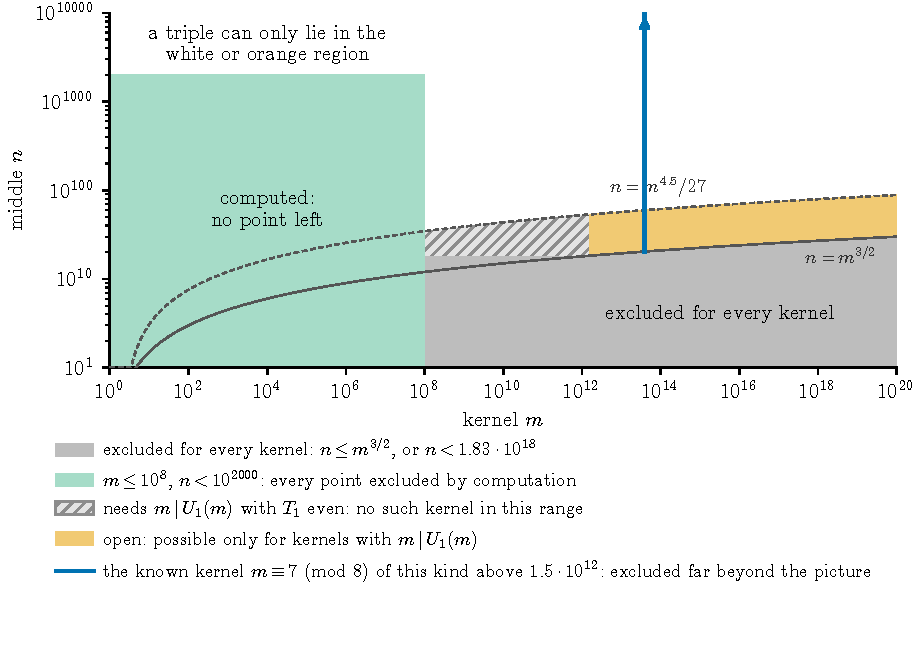
\includegraphics[width=\textwidth]{fig_kartemn}
\caption{\textbf{Where a triple could still lie.} The kernel $m$ on a logarithmic scale, the middle $n$ on a doubly logarithmic one. Gray:
excluded for every kernel, by the height bound of Corollary~\tref{cor:kern} or by Proposition~\tref{prop:paarliste}(d). Hatched: here a middle
needs $m \mid U_1(m)$ with $T_1(m)$ even, and Reinhart's complete list has no such kernel between $\Z{kernschranke}$ and $1.5 \cdot 10^{12}$
(Remark~\tref{rem:reinhartliste}; the parity of $T_1$ is computed in Proposition~\tref{prop:reinhart}). Green: the box of Theorem~\tref{thm:reduktion}, where every lattice point is excluded by computation.
Orange: the weak point of the bound, kernels with $m \mid U_1(m)$ above $1.5 \cdot 10^{12}$ (Question~\tref{q:walsh}); the one known kernel of
this kind above $1.5 \cdot 10^{12}$ in class~$7$ with $T_1$ even, drawn as a line, admits no middle below the height given in
Table~\ref{tab:reinhart}, and so does the other known one, which lies in the box. The picture does not draw the classes of kernels that
Section~\tref{sec:gebiete} excludes, so a triple could lie only in parts of the white and orange regions.}\label{fig:kartemn}
\end{figure}

A positive integer is \emph{powerful} if every prime that divides it divides it at least twice. Erd\H{o}s asked whether three consecutive
integers can all be powerful, and conjectured that they cannot \cite{Erdos1976Manitoba,Bloom364}; on the attribution among Erd\H{o}s's
papers see \cite[Section~7]{BajpaiBennettChan2024}. Mollin and Walsh conjectured it in a form about Pell numbers \cite[p.~111]{MollinWalsh1986a}
(Section~\tref{sec:exponent}). Two consecutive powerful
numbers exist in abundance, since $x^2 - 8y^2 = 1$ has infinitely many solutions, and four consecutive ones are impossible, since one of
four consecutive integers is $2$ modulo $4$. No triple is known. The $abc$ conjecture implies that there are only finitely many, and its
explicit forms give finite bounds (Remark~\tref{rem:abc}); unconditionally the question is open. Bloom records that no triple has a
middle below $7.38 \cdot 10^{28}$ by OEIS A076445 \cite{Bloom364,OEISA076445}, a statement that rests on the listed terms of that sequence
(Section~\tref{sec:daten}).

We expect that there is no triple, and we give the reasons as evidence, not as proof. First, the $abc$ conjecture implies that there are
at most finitely many (Remark~\tref{rem:abc}). Second, none has been found: none has a middle below $\Z{ohnetripelsicher}$
(Proposition~\tref{prop:paarliste}(d)), and none lies below $10^{22}$ by an enumeration of pairs that is described as exhaustive but is
not certified \cite{OEISA060355,MianSiddique2026}. Mian and Siddique prove, with machine-checked theorems in Lean~4, that no triple lies
below $10^{14}$ \cite{MianSiddique2026}; Table~\ref{tab:schranken} lists these bounds with what each rests on. Third, a triple needs a powerful Pell number $T_k(m)$, and this means that for each
divisor $d \ge 5$ of $k$ with $k < d(4d - 1)$ every prime of rank $d$, and there is at least one, must divide $T_d(m)$ at least twice (Corollary~\tref{cor:teiler});
at our \Z{bedpunkte} lattice points the median number of such conditions is \Z{bedmedian} (Proposition~\tref{prop:teilerdaten}). In the
data, a prime $p$ divides the first Pell term that it divides at least twice about as often as the model with probability $1/p$ predicts
(Proposition~\tref{prop:exponenten}); under that model each condition is one more rare event. The third reason is a heuristic, and the
model is not proved.

\begin{table}[ht]
\centering
\small
\begin{tabular}{l p{7.4cm} l}
\hline
no triple below & what the bound rests on & source \\
\hline
$10^{14}$ & machine-checked theorems in Lean~4 & \cite{MianSiddique2026} \\
$\Z{ohnetripelsicher}$ & computation in this part, every witness proved prime, together with Reinhart's computer proof that his list of the
  kernels dividing $U_1$ is complete up to $1.5 \cdot 10^{12}$ & Proposition~\tref{prop:paarliste}(d) \\
$\Z{ohnetripel}$ & the same, if Reinhart's extended search missed nothing & Proposition~\tref{prop:paarliste}(d) \\
$10^{22}$ & an enumeration of the pairs, described as exhaustive, not certified & \cite{OEISA060355,MianSiddique2026} \\
$7.38 \cdot 10^{28}$ & the listed terms of OEIS A076445; the entry does not state that the list is complete & \cite{Bloom364,OEISA076445} \\
\hline
\end{tabular}
\caption{\textbf{Bounds below which no triple of consecutive powerful numbers is known, and what each rests on.} Our two rows and the last one bound the
middle of a triple; the rows for $10^{14}$ and $10^{22}$ are stated for the triple, whose members differ from its middle by at most one.}\label{tab:schranken}
\end{table}

The problem has an exact address system, due to Mollin and Walsh, Walker and Sentance (Lemmas~\tref{lem:kriterium} to~\tref{lem:gerademitte}):
the middle $n$ of a triple is a term $T_k(m)$ of the Pell sequence of a squarefree kernel $m \equiv 7 \pmod 8$, at an odd index $k$ that is
a multiple of the part $m'$ of $m$ prime to $U_1$. So a triple is a lattice point $(m, k)$ at which $T_k(m)$ is even and powerful, and the question
becomes a question about the prime factors of Pell numbers. Two facts make it hard. Granville showed that the nonexistence of triples
implies that there are infinitely many primes $p$ with $p^2 \nmid 2^p - 2$ (Theorem~\tref{cor:wieferich}), a statement that is not known
unconditionally; so a proof would also settle an open problem about Wieferich primes. And an $abc$ inequality with exponent below $4/3$
would exclude all large triples, while the exponents derived from the explicit form of the conjecture, itself unproved, are $1.7$ and more
(Remark~\tref{rem:abc}).

This part does three things. It proves a height inequality that bounds the middle of a triple from below in terms of its kernel, and
splits the kernels into two wings by whether $m$ divides $U_1(m)$. It recasts the reduction of Mollin and Walsh as a statement about
witnesses, primes that divide a Pell number exactly once, and organizes the witnesses by their rank. And it computes: every lattice point
with kernel up to $\Z{kernschranke}$ and $T_k < 10^{\Z{hoehe}}$ is excluded by a certified witness or by parity, and of the \Z{rgpaare}
building blocks $\Prim{d}$ that occur there, \Z{rgzert} are shown not to be powerful by a certified witness, a prime that divides the block exactly once and is proved prime;
\Z{rgoffen} remain open. The weak point of the bound is wing~(ii), the kernels with $m \mid U_1$: for
them only $n > m^{3/2}$ is available, all such kernels up to $1.5 \cdot 10^{12}$ are known \cite[Remark~5.5]{Reinhart2023}, up to
$5.325 \cdot 10^{13}$ with a caveat of the author \cite{Reinhart2024}, and beyond that we know no lower bound for their middles other than
$n > m^{3/2}$ (Section~\tref{sec:hoehe}). Part~II meets the kernels with $m \mid U_1(m)$ and $T_1(m)$ even, of both residue classes, from
the side of pairs, and the collected volume lists the open problems of both parts together.

\paragraph{Main results.}
\begin{itemize}
\item \emph{The height inequality} (Theorem~\tref{thm:hoehe}): at every lattice point,
  \[
    \log_{10} T_k(m) \ \ge\ m'\bigl(1.5 \log_{10} m - \log_{10} m'\bigr) - \log_{10} 2 .
  \]
  With Remark~\tref{rem:siebenundzwanzig}, a triple with middle below $10^H$ has its kernel in one of two wings (Corollary~\tref{cor:fluegel}): $m \nmid U_1$ and
  $m < (27 \cdot 10^H)^{2/9}$, or $m \mid U_1$ and $m < 10^{2H/3}$.
\item \emph{The reduction theorem} (Theorem~\tref{thm:reduktion}): among the \Z{kerne} kernels up to $\Z{kernschranke}$, exactly \Z{punkte}
  lattice points have $T_k < 10^{\Z{hoehe}}$; \Z{paritaetspunkte} of them have $T_k$ odd, and each of the other \Z{zeugenpunkte} has a certified
  witness below $\Z{zeugenschranke}$. So no triple has a middle $n < 10^{\Z{hoehe}}$ with $\operatorname{sqfree}(n^2 - 1) \le \Z{kernschranke}$,
  and no triple at all has a middle below $\Z{ohnetripelsicher}$ (Proposition~\tref{prop:paarliste}(d)).
\item \emph{The witness statement} (Theorem~\tref{thm:zeugen}): there is no triple if and only if every lattice point with $T_1(m)$ even has a witness, and
  a witness can then be found among the primes whose rank divides $k$ with odd cofactor; a powerful $T_k$ would also have to satisfy the
  exponent-$3$ condition of Proposition~\tref{prop:exp3}. The $b$-box (Theorem~\tref{thm:bbox}) excludes every middle, of any size, with
  kernel up to $\Z{bboxkern}$ and squarefree part up to $\Z{bboxb}$; the strip (Theorem~\tref{thm:streifen}) shows that a triple with
  kernel up to $\Z{streifenschranke}$ has a middle of more than $\Z{streifenstellen}$ digits; the smooth kernels (Theorem~\tref{thm:glatt})
  exclude a further range below $10^{\Z{glatthoehe}}$.
\item \emph{The building blocks} (Proposition~\tref{prop:raenge}): of the \Z{rgpaare} primitive parts $\Prim{d}$ on the \Z{rgkerne} kernels of
  the lattice points, \Z{rgzert} have a certified witness; \Z{rgoffen} are open,
  each with at least \Z{offenmin} digits. Theorem~\tref{thm:profil} collects the conditions on a counterexample that this part proves or computes.
\end{itemize}

\paragraph{How to read this part.} Every statement is followed by a paragraph \emph{In words} that says what it means with as few formulas
as possible; a reader who wants the results can read the statements and these paragraphs. A reader who wants to check can read the proofs,
the paragraphs \emph{The computation}, and the tables; every number we computed is generated from the data files of the deposit or from a
cited constant, and every
numbered statement carries a label that says whether it is proved, taken from the literature, computed, measured, a heuristic, or open (see
the table at the end). A statement that combines several kinds carries the label of the part that needs the most trust: a proof that uses our own computation is labeled computed, and a proof that uses a published result is labeled proved. Table~\ref{tab:legende} collects the notation.

\paragraph{Plan.} The rest of this section sets up the notation and the address system. Section~\tref{sec:hoehe} proves the height
inequality and the two wings. Section~\tref{sec:reduktion} states the reduction theorem and describes the computation behind it.
Section~\tref{sec:exponent} proves the exponent condition and the reduction to a witness statement, computes the $b$-box, and records Granville's
theorem. Section~\tref{sec:gebiete} adds the strip, the smooth kernels and the square-type middles. Section~\tref{sec:daten} reports the
data: the exponents at the rank, the list of pairs at distance two, the ladders for the known kernels dividing $U_1$, the witnesses, and the
building blocks. Section~\tref{sec:profil} collects the profile of a counterexample, Section~\tref{sec:routen} records the routes that do
not close the problem, and Section~\tref{sec:fragen} states the open questions.


\subsection{Notation}
A positive integer $n$ is \emph{powerful} if $p^2$ divides $n$ for every prime $p$ that divides $n$.
For a squarefree integer $m \ge 2$ let $\varepsilon_m = T_1 + U_1\sqrt{m}$ be the fundamental solution of $x^2 - m y^2 = 1$,
that is, the solution in positive integers with the smallest $x$. For $k \ge 1$ write
\[
  \varepsilon_m^{\,k} = T_k + U_k\sqrt{m},
\]
and $T_k(m)$, $U_k(m)$ when the kernel $m$ has to be named. Put
\[
  m' = \prod_{p \mid m,\ p \nmid U_1} p,
\]
the product of the primes of $m$ that do not divide $U_1$. For an integer $N \ge 1$ let $\operatorname{sqfree}(N)$ be the product of the
primes that divide $N$ to an odd power.

\inwords A number is powerful when every prime in it appears at least twice; for example $72 = 2^3 \cdot 3^2$ is powerful and $12 = 2^2 \cdot 3$
is not. The equation $x^2 - m y^2 = 1$ is Pell's equation. Its smallest solution $\varepsilon_m$ produces all other solutions as powers, and
$T_k$ and $U_k$ are the two parts of the $k$-th power. The number $m'$ collects the primes of $m$ that do not divide $U_1$.

\subsection{The address system}

\begin{lemma}[Mollin and Walsh {\cite[Theorem, p.~110]{MollinWalsh1986a}}]\tlabel{lem:kriterium}\belegart{literature}
There are three consecutive powerful numbers if and only if there are a squarefree $m \equiv 7 \pmod 8$ and an odd $k$ such that
$T_k(m)$ is an even powerful number and $m$ divides $U_k(m)$. In that case the triple is $(T_k - 1, T_k, T_k + 1)$, and
$m = \operatorname{sqfree}(T_k^2 - 1)$.
\end{lemma}

Mollin and Walsh state the criterion with the fundamental unit of $\mathbb{Q}(\sqrt{m})$. For $m \equiv 7 \pmod 8$ this unit is
$\varepsilon_m$: the ring of integers is $\mathbb{Z}[\sqrt{m}]$, and $m$ has a prime factor $\equiv 3 \pmod 4$, so no unit of norm $-1$ exists.

\inwords The middle $n$ of a triple of consecutive powerful numbers is always even, and it is a Pell number $T_k$ for exactly one kernel $m$.
So the search for triples becomes a search over pairs $(m, k)$.

\begin{lemma}[Walker {\cite[Theorems 2.2(3) and 2.5]{Walker1976}}; Mollin and Walsh {\cite[p.~111]{MollinWalsh1986a}}]\tlabel{lem:walker}\belegart{literature}
Let $m$ be squarefree and let $p$ be a prime dividing $m$. Then $p \mid U_k$ if and only if $p \mid k U_1$. Hence $m \mid U_k$ if and only
if $m' \mid k$.
\end{lemma}

\begin{proof}
By the binomial theorem, $U_k = \sum_{i \text{ odd}} \binom{k}{i} T_1^{k-i} U_1^{\,i} m^{(i-1)/2}$. For $p \mid m$ every term with $i \ge 3$ is
divisible by $p$, so $U_k \equiv k T_1^{k-1} U_1 \pmod p$. From $T_1^2 - m U_1^2 = 1$ we get $T_1^2 \equiv 1 \pmod p$, so $T_1$ is invertible
modulo $p$, and the first claim follows. A prime $p \mid m$ with $p \mid U_1$ divides every $U_k$; a prime $p \mid m$ with $p \nmid U_1$
divides $U_k$ exactly when $p \mid k$. Since $m$ is squarefree, this gives the second claim.
\end{proof}

\inwords Whether $m$ divides $U_k$ depends only on whether $k$ is a multiple of $m'$. So for each kernel the useful indices $k$ are
exactly the multiples of $m'$.

\begin{lemma}[Sentance {\cite[Theorem and Converse, p.~272]{Sentance1981}}]\tlabel{lem:adresse}\belegart{literature}
Let $n \equiv 0 \pmod 4$. Then $n - 1$ and $n + 1$ are both powerful if and only if $n = T_k(m)$ for a squarefree $m \equiv 7 \pmod 8$ and
an odd $k$ with $m' \mid k$.
\end{lemma}

\begin{proof}
($\Leftarrow$) We have $n^2 - 1 = m U_k^2$ and $m \mid U_k$ by Lemma~\tref{lem:walker}, so $n^2 - 1 = m^3 w^2$ for an integer $w$. As $n$ is
even, $n - 1$ and $n + 1$ are coprime, so for every prime $p$ the full power of $p$ in $m^3 w^2$ lies in one of them. Hence each of
$n \pm 1$ has the form $a^3 s^2$ with $a \mid m$ squarefree, and such a number is powerful.
($\Rightarrow$) If $n \pm 1$ are powerful and coprime, then $N = n^2 - 1$ is powerful. Write $N = a^2 b^3$ with $b$ squarefree; then
$N = b (ab)^2$ with $b \mid ab$. So $(n, ab)$ solves $x^2 - b y^2 = 1$, and $(n, ab) = (T_k, U_k)$ for $m = b$ and some $k \ge 1$. From
$n \equiv 0 \pmod 4$ we get $n^2 - 1 \equiv 7 \pmod 8$; as $U_k$ is odd, $m \equiv 7 \pmod 8$. An even $T_k$ forces $k$ odd, since
$T_{2j} = 2T_j^2 - 1$ is odd. Finally $m \mid U_k$ gives $m' \mid k$ by Lemma~\tref{lem:walker}.
\end{proof}

\begin{lemma}[Sentance {\cite[p.~272]{Sentance1981}}; Mollin and Walsh {\cite[Lemma~1.1]{MollinWalsh1986b}}]\tlabel{lem:gerademitte}\belegart{literature}
(General even middle.) Let $n \ge 2$ be even. Then $n - 1$ and $n + 1$ are both powerful if and only if $n = T_k(m)$ for a squarefree odd $m \ge 3$ and an odd $k$
with $m' \mid k$ and $T_1(m)$ even. The pair $(m, k)$ is unique: $m = \operatorname{sqfree}(n^2 - 1)$, and $k$ is determined because $T_k$
increases with $k$. Moreover $m \equiv 7 \pmod 8$ if and only if $n \equiv 0 \pmod 4$, and $m \equiv 3 \pmod 8$ if and only if
$n \equiv 2 \pmod 4$; kernels $m \equiv 1, 5 \pmod 8$ never occur. An odd $n$ never occurs.
\end{lemma}

\begin{proof}
As for Lemma~\tref{lem:adresse}; only the residues change. For $n \equiv 2 \pmod 4$ we get $n^2 - 1 \equiv 3 \pmod 8$, and with $U_k$ odd,
$m \equiv 3 \pmod 8$. For odd $k$ we have $T_k \equiv T_1 \pmod 2$: if $T_1$ is even, every term of
$T_k = \sum_j \binom{k}{2j} T_1^{k-2j} (m U_1^2)^j$ contains a factor $T_1$; if $T_1$ is odd, every term with $j \ge 1$ contains the even
factor $m U_1^2 = T_1^2 - 1$. So $T_k$ is even exactly when $T_1$ is. If $n$ were odd, $n \pm 1$ would be even powerful numbers, hence both
divisible by $4$, which is impossible at distance two.
\end{proof}

The residue split and the uniqueness statement are added here; the rest is Sentance's theorem.

We call a pair $(m, k)$ with $m \equiv 7 \pmod 8$ squarefree and $k$ an odd multiple of $m'$ a \emph{lattice point}. By
Lemma~\tref{lem:adresse}, the lattice points with $T_k$ even are exactly the pairs of powerful numbers at distance two whose middle is
$\equiv 0 \pmod 4$. By Lemma~\tref{lem:kriterium}, a triple needs one more condition: $T_k$ itself must be powerful.

\inwords Two powerful numbers that differ by $2$ always sit around a Pell number $T_k$. So every such pair has an address $(m, k)$, and each
address carries at most one pair. A triple is a pair whose middle is powerful as well. The kernel also tells the remainder: $m \equiv 7
\pmod 8$ exactly when the middle is a multiple of $4$, and $m \equiv 3 \pmod 8$ when it is $2$ more than a multiple of $4$.

\subsection{Notation and terms at a glance}\tlabel{sec:legende}

Table~\ref{tab:legende} collects the symbols and words used in this part, with the place where each is defined.

\begin{table}[ht]
\centering
\small
\begin{tabular}{p{3.2cm} p{8.2cm} l}
\hline
symbol or term & meaning & defined in \\
\hline
powerful & every prime factor occurs at least twice & \S\tref{sec:adresse} \\
$v_p(N)$ & the exponent of the prime $p$ in $N$ & standard \\
$\operatorname{sqfree}(N)$ & the product of the primes that divide $N$ to an odd power & \S\tref{sec:adresse} \\
kernel $m$ & a squarefree $m \ge 2$; for a middle $n$ it is $m = \operatorname{sqfree}(n^2 - 1)$ & Lemma~\tref{lem:gerademitte} \\
$\varepsilon_m$, $T_k$, $U_k$ & the smallest solution $T_1 + U_1\sqrt{m}$ of $x^2 - my^2 = 1$, and its $k$-th power $T_k + U_k\sqrt{m}$
  & \S\tref{sec:adresse} \\
$m'$ & the product of the primes of $m$ that do not divide $U_1$ & \S\tref{sec:adresse} \\
address $(m, k)$ & the pair with $n = T_k(m)$ for a middle $n$ & Lemma~\tref{lem:adresse} \\
lattice point & a pair $(m, k)$ with $m \equiv 7 \pmod 8$ squarefree and $k$ an odd multiple of $m'$ & \S\tref{sec:adresse} \\
wings (i), (ii) & kernels with $m \nmid U_1$, and with $m \mid U_1$ & Corollary~\tref{cor:fluegel} \\
rank $\alpha_m(p)$ & the smallest $k \ge 1$ with $p \mid T_k(m)$ & Lemma~\tref{lem:rang} \\
witness & a prime that divides a number exactly once, which shows that the number is not powerful; the number is mostly $T_k(m)$ or
  $\Prim{d}$ & Theorem~\tref{thm:zeugen} \\
class $7$, class $3$ & kernels $m \equiv 7$, resp.\ $3 \pmod 8$; they belong to middles $n \equiv 0$, resp.\ $2 \pmod 4$
  & Lemma~\tref{lem:gerademitte} \\
$\tau(k)$ & the number of divisors of $k$ & standard \\
$\operatorname{rad}(N)$ & the product of the distinct primes dividing $N$ & standard \\
primitive part $\Prim{d}$, building block & the part of $T_d(m)$ on the primes of rank exactly $d$ & Proposition~\tref{prop:raenge} \\
$\Kreis{n}$ & the $n$-th cyclotomic polynomial & standard \\
Wieferich prime (to base $2$) & a prime $p$ with $p^2 \mid 2^{p-1} - 1$ & standard \\
Wieferich prime for $\varepsilon_m$ & an odd prime $p \nmid m$ with $p^2 \mid T_{\alpha_m(p)}(m)$ & Proposition~\tref{prop:lucaswieferich} \\
$abc$ conjecture & $c < C_\epsilon \operatorname{rad}(abc)^{1 + \epsilon}$ for coprime $a + b = c$ and every $\epsilon > 0$
  & Remark~\tref{rem:abc} \\
certified prime & a prime proved by a deterministic test or by a certificate that a second program checks & Proposition~\tref{prop:raenge} \\
$\psi_{12}$ & the smallest number that passes the strong test to the first twelve prime bases without being prime,
  $318\,665\,857\,834\,031\,151\,167\,461$ \cite{SorensonWebster2017} & Proposition~\tref{prop:raenge} \\
$V_n$ & the Lucas sequence $V_n(2T_1, 1) = 2T_n$ & Proposition~\tref{prop:raenge} \\
$B_1$ & the first-stage bound of the elliptic curve method & Table~\ref{tab:offen} \\
\hline
\end{tabular}
\caption{Symbols and terms of Part I.}\label{tab:legende}
\end{table}

\section{The height inequality}\tlabel{sec:hoehe}

\begin{theorem}[height inequality]\tlabel{thm:hoehe}\belegart{proved}
Let $m \equiv 7 \pmod 8$ be squarefree and let $k$ be an odd multiple of $m'$, so that $m \mid U_k$. Then
\[
  \log_{10} T_k(m) \ \ge\ m' \bigl(1.5 \log_{10} m - \log_{10} m'\bigr) - \log_{10} 2 .
\]
In particular this bound holds for the middle $n = T_k \equiv 0 \pmod 4$ of every pair of powerful numbers at distance two, and so for the
middle of every triple of consecutive powerful numbers.
\end{theorem}

\begin{proof}
Put $d = m/m'$. By definition $d$ divides $U_1$, so $U_1 \ge d$. Hence $T_1 = \sqrt{m U_1^2 + 1} > \sqrt{m}\, U_1 \ge m^{3/2}/m'$. Since
$T_k = (\varepsilon_m^k + \varepsilon_m^{-k})/2 \ge \varepsilon_m^k/2 \ge T_1^k/2$ and $k \ge m'$, we get
$T_k \ge T_1^{m'}/2 > (m^{3/2}/m')^{m'}/2$. Take logarithms.
\end{proof}

\inwords The larger $m'$ is, the larger the middle must be: its number of digits exceeds $m' \log_{10}(m^{1.5}/m') - 1$. This already
forces the middle of any triple with a large $m'$ to be enormous.

We did not find this inequality in the literature. Aktaş and Murty \cite[proof of Theorem~1.3, p.~251]{AktasMurty2017} bound the index
using only the trivial lower bound for the fundamental solution, and Chan \cite[Section~2]{Chan2012} counts solutions of Thue equations; neither uses
that $m'$ divides the index. Mollin and Walsh \cite[p.~111]{MollinWalsh1986a} and Stephens and Williams \cite[p.~619]{StephensWilliams1988}
note that $k$ must be large.

\begin{remark}[the constant in the height bound]\tlabel{rem:siebenundzwanzig}\belegart{proved}
All terms of the binomial expansion $T_k = \sum_j \binom{k}{2j} T_1^{k-2j} (m U_1^2)^j$ are nonnegative, so $T_k \ge T_1^k$. Hence the term
$-\log_{10} 2$ in Theorem~\tref{thm:hoehe} can be dropped:
\[
  T_k \ \ge\ \bigl(m^{3/2}/m'\bigr)^{m'} .
\]
The proof uses only that $m$ is odd and squarefree and that $m' \mid k$. So the same bound holds for kernels $m \equiv 3 \pmod 8$, which
carry the pairs with middle $\equiv 2 \pmod 4$ (Lemma~\tref{lem:gerademitte}).
\end{remark}

\inwords A slightly better bound holds, without the factor $1/2$, and it holds for both kinds of even middles.

\begin{corollary}[kernel bound]\tlabel{cor:kern}\belegart{proved}
Let $m$ and $k$ be as in Theorem~\tref{thm:hoehe}. If $m \nmid U_1$, then $T_k > m^{4.5}/27$. If $m \mid U_1$, then $T_k \ge T_1 > m^{3/2}$.
\end{corollary}

\begin{proof}
If $m \nmid U_1$, then $m' > 1$, and $m'$ is odd, so $m' \ge 3$. By Remark~\tref{rem:siebenundzwanzig},
$\ln T_k \ge f(m')$ with $f(x) = x (1.5 \ln m - \ln x)$. Since $f'(x) = 1.5 \ln m - \ln(e x)$, the function $f$ increases on $[3, m]$ as
soon as $m^{3/2}/e > m$, that is, for $m \ge 8$. As $m' \le m$, we get $\ln T_k \ge f(3) = 4.5 \ln m - 3 \ln 3$, which is the claim. The only
kernel below $8$ is $m = 7$, where $m' = 7$; there the smallest term is $T_7(7) \ge T_1(7)^7 = 8^7$, far above $7^{4.5}/27$.
If $m \mid U_1$, then $U_1 \ge m$, so $T_1 > \sqrt{m}\, U_1 \ge m^{3/2}$, and $T_k \ge T_1$.
\end{proof}

\inwords If $m$ does not divide $U_1$, the middle is larger than $m^{4.5}/27$. If $m$ divides $U_1$, we only know that the middle is
larger than $m^{1.5}$.

\begin{corollary}[two wings]\tlabel{cor:fluegel}\belegart{proved}
Let $H > 0$. Let $n < 10^H$ be the middle of a triple of consecutive powerful numbers, or the middle $n \equiv 0 \pmod 4$ of a pair of
powerful numbers at distance two, and let $m = \operatorname{sqfree}(n^2 - 1)$. Then
\begin{enumerate}
  \item[(i)] either $m \nmid U_1$ and $m < (27 \cdot 10^H)^{2/9}$,
  \item[(ii)] or $m \mid U_1$ and $m < 10^{2H/3}$.
\end{enumerate}
\end{corollary}

\begin{proof}
By Lemmas~\tref{lem:kriterium} and \tref{lem:adresse}, $n = T_k(m)$ for a lattice point $(m, k)$. In case $m \nmid U_1$,
Corollary~\tref{cor:kern} gives $m^{4.5}/27 < n < 10^H$; in case $m \mid U_1$ it gives $m^{3/2} < n < 10^H$.
\end{proof}

\inwords Every triple below $10^H$ has its kernel in one of two ranges. We call them wing~(i), for kernels that do not divide $U_1$, and
wing~(ii), for kernels that do. Wing~(ii) allows much larger kernels.

The condition that separates the wings, $m \mid U_1$ or not, has an exact description by Wieferich primes in number fields, due to Fellini
and Murty \cite[Theorem~1.1]{FelliniMurty2026}. We use only the different height behavior of the two wings.

Wing~(ii) is the weak side. For a kernel with $m \mid U_1$ only the bound $n > m^{3/2}$ of Corollary~\tref{cor:kern} is available. All such
kernels up to $1.5 \cdot 10^{12}$ are known, and up to $5.325 \cdot 10^{13}$ if Reinhart's extended search missed nothing
(Remark~\tref{rem:reinhartliste}); above that we know nothing about their size beyond Corollary~\tref{cor:kern}. A lower bound for $T_1(m)$ that grows faster with $m$ in this class would close this gap, and we do not have one.
Park \cite{Park2012} proves lower bounds for fundamental units that hold for almost all members of certain families. A statement about almost
all members does not exclude a single exception, so it does not close the gap.

\begin{remark}[Reinhart's list]\tlabel{rem:reinhartliste}\belegart{literature}
The squarefree $m$ with $m \mid U_1(m)$ are the members of OEIS A135735 \cite{OEISA135735}. Reinhart proved by computer search that the
list is complete up to $1.5 \cdot 10^{12}$ \cite[Remark~5.5]{Reinhart2023}. His later search covers the squarefree $m$ up to
$5.325 \cdot 10^{13}$ and found four further members, but he writes that he does not claim that these are all the members in that range,
for lack of an independent double check, and that it is likely that all were found \cite[Section~3]{Reinhart2024}. We therefore keep two
bounds apart: below $1.5 \cdot 10^{12}$ the list is complete; below $5.325 \cdot 10^{13}$ it is complete if the extended search missed
nothing. Every statement that uses the larger bound says so. Of the members $m \equiv 7 \pmod 8$, \Z{reinhartsiebensicher} lie below the
smaller bound and \Z{reinhartsieben} below the larger one.
\end{remark}

\inwords A published list of the dangerous kernels exists. Up to $1.5 \cdot 10^{12}$ its author proved it complete. Up to
$5.325 \cdot 10^{13}$ he searched everything, but could not afford a second, independent run, and says so. We keep the two levels apart, and
every statement below names the one it uses.

\section{The reduction theorem}\tlabel{sec:reduktion}

\begin{theorem}[reduction]\tlabel{thm:reduktion}\belegart{computed}
Among the $\Z{kerne}$ squarefree $m \equiv 7 \pmod 8$ with $m \le \Z{kernschranke}$, exactly $\Z{filterfamilien}$ pass the discard criterion
described below, and $\Z{punktfamilien}$ of these have an odd multiple $k$ of $m'$ with $T_k(m) < 10^{\Z{hoehe}}$. Together they have
exactly $\Z{punkte}$ such indices $k$. For $\Z{paritaetspunkte}$ of them $T_k$ is odd. For each of the remaining $\Z{zeugenpunkte}$ there is a
prime $p < \Z{zeugenschranke}$ that divides $T_k$ exactly once. Consequently, there is no triple of consecutive powerful numbers whose
middle $n$ satisfies $n < 10^{\Z{hoehe}}$ and $\operatorname{sqfree}(n^2 - 1) \le \Z{kernschranke}$.
\end{theorem}

\begin{proof}
By Lemma~\tref{lem:kriterium}, such a triple is a lattice point $(m, k)$ with $m \le \Z{kernschranke}$ and $T_k < 10^{\Z{hoehe}}$ at which
$T_k$ is even and powerful. An odd $T_k$ fails the first condition. A prime that divides $T_k$ exactly once shows that $T_k$ is not powerful.
It remains to check that the list of points is complete, which is the computation below.
\end{proof}

\inwords We checked every possible address with a kernel up to $\Z{kernschranke}$ and a middle below $10^{\Z{hoehe}}$. At each of the
$\Z{punkte}$ addresses, either the middle is odd, or a small prime divides it only once. In both cases the middle is not powerful, so no
triple lives there. The theorem says nothing about kernels above $\Z{kernschranke}$ or middles above $10^{\Z{hoehe}}$.

\paragraph{The computation.}
Put $H = \Z{hoehe}$. For each $m \le \Z{kernschranke}$ the continued fraction of $\sqrt{m}$ is computed twice: modulo $m$, which gives
$U_1 \bmod m$ and hence $m'$ by Lemma~\tref{lem:walker}, and in scaled floating point, which gives $\log_{10} T_1$; on a sample of \Z{fpn} kernels, all up to $2 \cdot 10^4$ and the others
drawn at random up to $10^8$, its relative error against the exact value is below $\Z{fpmax}$. A kernel is discarded when $m' > (H + 0.31)/\log_{10} T_1 + 1$. This is rigorous: for every admissible $k$,
$\log_{10} T_k \ge k \log_{10} T_1 - 0.31 \ge m' \log_{10} T_1 - 0.31$, so a discarded kernel has no index with $T_k < 10^H$; the extra $1$
is a margin against rounding. It absorbs any relative error in $\log_{10} T_1$ up to $\log_{10} T_1/(H + 0.31)$, and since $T_1 \ge 4$ for
every $m \equiv 7 \pmod 8$, an error below $3 \cdot 10^{-4}$ is enough, and the measured error is far below that.
For the $\Z{filterfamilien}$ surviving kernels the unit is computed exactly and compared with the modular
route, and the run stops on any mismatch. Each $T_k < 10^H$ is computed exactly and tested for parity and for a prime
$p < \Z{zeugenschranke}$ with $v_p(T_k) = 1$. The discard criterion was also rechecked without floating point, from the bound
$\log_{10} T_1 \ge (\ell - 1)\log_{10}\varphi - \log_{10}\sqrt{5}$, where $\ell$ is the period length of the continued fraction and
$\varphi$ the golden ratio; the numerators of the convergents grow at least like Fibonacci numbers. This was done for a random sample of $\Z{margestich}$ discarded kernels
up to $\Z{margemax}$ and for every discarded kernel up to $\Z{margerand}$: none is contradicted, and the smallest margin by
which a discarded kernel exceeds $10^H$ is $\Z{margemin}$ orders of magnitude. Three versions of the scan, which differ in speed and not in the
criterion, give identical lists of points and witnesses. The list of points with their witnesses is part of the data deposit. Figure~\ref{fig:trichter} shows the numbers.

\begin{figure}[ht]
\centering
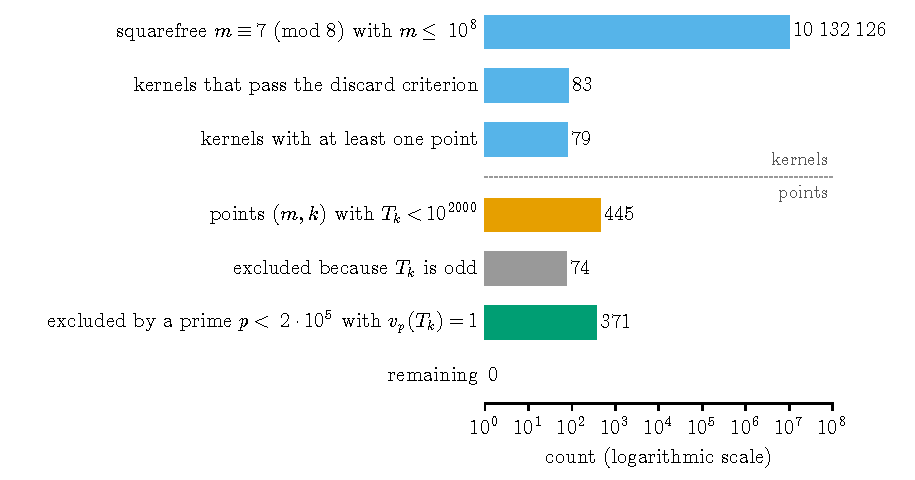
\includegraphics[width=\textwidth]{fig_trichter}
\caption{\textbf{No point of the box remains.} From all kernels to no candidate (Theorem~\tref{thm:reduktion}). The horizontal axis is logarithmic. The upper three bars count
kernels, the lower ones count points $(m, k)$; the two exclusions add up to all points, and none remains.}\label{fig:trichter}
\end{figure}

\paragraph{An example.}
Of the $\Z{punkte}$ points, the one with the smallest middle is $(m, k) = (\Z{beispielm}, \Z{beispielk})$, the example of Mollin and
Walsh \cite[p.~111]{MollinWalsh1986a}. There $\varepsilon_7 = 8 + 3\sqrt{7}$, so $7 \nmid U_1$ and $m' = m$, and
\[
  n = T_{\Z{beispielk}}(\Z{beispielm}) = \Z{beispielwert} = \Z{beispielfaktoren}.
\]
Since $n \equiv 0 \pmod 4$ and $m'$ divides $k$, Lemma~\tref{lem:adresse} shows that $n - 1$ and $n + 1$ are powerful. But the prime
$\Z{beispielzeuge}$ divides $n$ exactly once, so $n$ is not powerful, and $(n - 1, n, n + 1)$ is not a triple. The prime $\Z{beispielzeuge}$ is
the witness recorded for this point.

\begin{remark}[weaker bounds with less work]\tlabel{rem:ohnetripel}\belegart{proved}
The same method gives weaker bounds with less work. The list OEIS A135735 contains all squarefree $m$ with $m \mid U_1(m)$ up to
$1.5 \cdot 10^{12}$, and up to $5.325 \cdot 10^{13}$ if Reinhart's extended search missed nothing (Remark~\tref{rem:reinhartliste}). A
kernel with $m \mid U_1$ that is not on this list is therefore larger than $1.5 \cdot 10^{12}$, and Corollary~\tref{cor:kern} gives
$n > m^{3/2} > \Z{ohnetripelsicher}$ for every triple with such a kernel; under the assumption on the extended search the bound is
$\Z{ohnetripel}$. The
enumeration of consecutive powerful pairs behind the b-file of OEIS A060355 is described by Mian and Siddique as exhaustive below
$10^{22}$ but not certified \cite{OEISA060355,MianSiddique2026}; since every triple contains two such pairs, it excludes triples below that
bound on the same terms. The bound above is stated as Proposition~\tref{prop:paarliste}(d); here it only illustrates the method.
\end{remark}

\inwords A short list plus the height bound already pushes some triples beyond $\Z{ohnetripelsicher}$. This is only an illustration: other searches reach
further, and the reduction theorem is the actual result of this section.

\section{The exponent condition and the witness reduction}\tlabel{sec:exponent}

For a prime $p$ that does not divide $m$, this section describes at which indices $k$ it divides $T_k$, and with which exponent. This
turns the question whether $T_k$ is powerful into a question about finitely many primes.

\begin{lemma}[Bennett and Walsh {\cite[proof of Lemma~3.3, p.~3484]{BennettWalsh1999}}; Lehmer {\cite{Lehmer1930}}]\tlabel{lem:rang}\belegart{literature}
Let $p$ be a prime with $p \nmid m$. Either $p$ divides no $T_k$, or there is a smallest index $\alpha_m(p) \ge 1$ with
$p \mid T_{\alpha_m(p)}$. In the second case, $p \mid T_k$ if and only if $k$ is an odd multiple of $\alpha_m(p)$.
\end{lemma}

We call $\alpha_m(p)$ the \emph{rank} of $p$. Bennett and Walsh state the lemma in the proof of their Lemma~3.3 and characterize the rank in
their Lemma~5.1 \cite[p.~3486]{BennettWalsh1999}, where they call it quite standard and refer to Lehmer.

\inwords A prime appears in the sequence $T_1, T_2, T_3, \ldots$ for the first time at its rank $\alpha$. After that it divides exactly
the terms $T_{\alpha}, T_{3\alpha}, T_{5\alpha}, \ldots$, and no others.

\begin{lemma}[Bennett and Walsh {\cite[Theorem~1.2]{BennettWalsh1999}}]\tlabel{lem:quadratwert}\belegart{literature}
Let $m$ and $b > 1$ be squarefree. There is at most one index $k$ with $T_k = b x^2$ for an integer $x$, and if it exists, then
$k = \alpha_m(b)$, the smallest $k$ with $b \mid T_k$.
\end{lemma}

By Lemma~\tref{lem:rang}, $\alpha_m(b)$ exists if and only if every prime of $b$ has a rank and all these ranks have the same $2$-adic
valuation; then $\alpha_m(b)$ is their least common multiple.

\inwords A term $T_k$ can be $b$ times a square for at most one index $k$, and this index is the first place where $b$ divides the
sequence.

\begin{lemma}[valuation identity]\tlabel{lem:bewertung}\belegart{proved}
Let $p$ be an odd prime with $p \nmid m$ and $p \mid T_r$. Then $v_p(T_{rt}) = v_p(T_r) + v_p(t)$ for every odd $t$.
\end{lemma}

\begin{proof}
Here $v_p(z)$, for $z \in \mathbb{Z}[\sqrt{m}]$, is the largest $e$ with $p^e \mid z$ in $\mathbb{Z}[\sqrt{m}]$, the least $p$-adic valuation of the two
coefficients of $z$. It is not multiplicative when $p$ splits, but it does not change under multiplication by a unit or by an element congruent to $1$ modulo $p$, and
$v_p(tz) = v_p(t) + v_p(z)$ for $t \in \mathbb{Z}$; this is all that the standard proof of the lifting-the-exponent lemma uses.
Put $w = \varepsilon_m^{2r}$ and $u = w + 1 = \varepsilon_m^{r} \cdot 2T_r$, so $v_p(u) = v_p(T_r) \ge 1$. For odd $t$,
\[
  2T_{rt} = \varepsilon_m^{-rt}\,(w^t + 1) = \varepsilon_m^{-rt}\,\bigl(1 - (1 - u)^t\bigr),
\]
and the lifting-the-exponent lemma in $\mathbb{Z}[\sqrt{m}]$ gives $v_p(1 - (1 - u)^t) = v_p(u) + v_p(t)$. It applies because $p$ is odd,
$p \nmid m$, and $p$ divides $u$ but not $1 - u$; the proof is the same as for integers.
\end{proof}

\inwords If a prime $p$ divides $T_r$, then in $T_{rt}$ it appears exactly as often as in $T_r$, plus as often as it divides $t$. So a
prime that appears once in $T_r$ appears once in $T_{rt}$, unless it also divides $t$.

\begin{proposition}[exponent-3 condition]\tlabel{prop:exp3}\belegart{proved}
Let $T_k$ be an even powerful number with $k$ odd and $m' \mid k$, and let $b = \operatorname{sqfree}(T_k)$, so that $T_k = b^3 z^2$ for an
integer $z$. If $b > 1$, then $k = \alpha_m(b)$, and for every odd prime $p \mid b$
\[
  v_p\bigl(T_{\alpha_m(p)}\bigr) + v_p\bigl(\alpha_m(b)/\alpha_m(p)\bigr) \ \ge\ 3 .
\]
\end{proposition}

\begin{proof}
We have $T_k = b (bz)^2$, so $k = \alpha_m(b)$ by Lemma~\tref{lem:quadratwert}. Now let $p \mid b$ be odd. Then $p \mid T_k$, so $k = \alpha_m(p)\, t$ with $t$ odd by
Lemma~\tref{lem:rang}, and $v_p(T_k) = v_p(T_{\alpha_m(p)}) + v_p(t)$ by Lemma~\tref{lem:bewertung}. As $p$ divides the powerful number $T_k$ to an odd power, this power is
at least $3$.
\end{proof}

For general Lucas sequences the valuation identity is standard; see Sanna \cite{Sanna2016}. Ballot \cite[p.~265, (2)]{Ballot2019} printed
it with the term $(\nu - 1) + v_p(n)$, and the errata \cite{Ballot2019Errata} corrects this to $\nu + v_p(n/\rho)$. The corrected form is the
one in Lemma~\tref{lem:bewertung}. On $\Z{ballotfaelle}$ cases of our sequence, the corrected form holds in all of them and the printed form in
$\Z{ballotgedruckt}$; on $\Z{ballotfib}$ cases of the Fibonacci numbers, the corrected form holds in all of them.

\inwords If the middle $T_k$ is powerful, then every prime that divides it an odd number of times divides it at least three times. This
gives a condition on the first term $T_{\alpha(p)}$ in which the prime appears. Proposition~\tref{prop:exp3} does not prove the
conjecture of Mollin and Walsh \cite[p.~111]{MollinWalsh1986a} that $T_k$ is never an even powerful number for odd $k > 1$; it says what
a counterexample would have to satisfy.

\begin{theorem}[the $b$-box]\tlabel{thm:bbox}\belegart{computed}
There is no triple of consecutive powerful numbers whose middle $n$ has kernel $m \le \Z{bboxkern}$ and $\operatorname{sqfree}(n) \le
\Z{bboxb}$, whatever the size of $n$.
\end{theorem}

\begin{proof}
If $\operatorname{sqfree}(n) = 1$, then $n$ is a square, and Theorem~\tref{thm:quadratmitte} gives $m \mid U_1$; no such kernel with $T_1$
even lies below $\Z{bboxkern}$: the kernels $m \mid U_1$ below this bound are listed completely \cite[Remark~5.5]{Reinhart2023}, and the only one with
$m \equiv 7 \pmod 8$, $209\,991$, has $T_1$ odd (Theorem~\tref{thm:quadratmitte}; OEIS \cite{OEISA135735}). Otherwise let $b = \operatorname{sqfree}(n) > 1$ and $n = T_k(m)$. By
Proposition~\tref{prop:exp3}, $k = \alpha_m(b)$, so $\alpha_m(b)$ must exist, be odd and be a multiple of $m'$, and $b^3$ must divide
$T_{\alpha_m(b)}$. We checked all pairs. There are $\Z{bboxfam}$ squarefree $m \equiv 7 \pmod 8$ with $m \le \Z{bboxkern}$; for
$\Z{bboxparitaet}$ of them $T_1$ is odd, so they carry no even middle. The others give $\Z{bboxpaare}$ pairs $(m, b)$ with squarefree
$b \le \Z{bboxb}$, $b = 1$ included. In $\Z{bboxohnealpha}$ pairs some prime of $b$ has no rank, in $\Z{bboxzweiadisch}$ the ranks have different $2$-adic
valuations, in $\Z{bboxkgerade}$ the index $\alpha_m(b)$ is even, and in $\Z{bboxlemmal}$ it is not a multiple of $m'$; this class contains the pairs with $b = 1$, where $k = 1$ while $m' > 1$ for every
such kernel with $T_1$ even \cite{Reinhart2024}. For each of the
remaining $\Z{bboxrest}$ pairs, $b^3$ does not divide $T_{\alpha_m(b)}$; this is tested modulo $b^3$.
\end{proof}

\inwords If the kernel is at most $\Z{bboxkern}$ and the part of the middle with odd exponents is at most $\Z{bboxb}$, there is no triple,
however large the middle is. This result has no height limit, unlike Theorem~\tref{thm:reduktion}.

\begin{theorem}[reduction to a witness statement]\tlabel{thm:zeugen}\belegart{proved}
Let $\mathcal{L}$ be the set of lattice points $(m, k)$ with $T_1(m)$ even. For $(m, k) \in \mathcal{L}$ one has $4 \mid T_k(m)$ and
$\gcd(T_k(m), m) = 1$. The following statements are equivalent.
\begin{enumerate}
  \item[(i)] There are no three consecutive powerful numbers.
  \item[(ii)] For every $(m, k) \in \mathcal{L}$ there is a prime $p$ with $v_p(T_k(m)) = 1$, a \emph{witness}.
  \item[(iii)] For every $(m, k) \in \mathcal{L}$ there is an odd prime $p \nmid m$ such that $k$ is an odd multiple of $\alpha_m(p)$,
  $v_p(T_{\alpha_m(p)}(m)) = 1$, and $p \nmid k/\alpha_m(p)$.
\end{enumerate}
In particular, if $T_k(m)$ is powerful, then $p^2 \mid T_k(m)$ for every prime $p$ with $\alpha_m(p) = k$.
\end{theorem}

\begin{proof}
By Lemmas~\tref{lem:kriterium} and \tref{lem:adresse}, a triple exists if and only if $T_k(m)$ is powerful for some $(m, k) \in \mathcal{L}$.
For every $(m, k) \in \mathcal{L}$ the number $T_k$ is even (proof of Lemma~\tref{lem:gerademitte}), $U_k = m w$ by Lemma~\tref{lem:walker} with
$w$ odd, and $T_k^2 = 1 + m^3 w^2 \equiv 1 + 7 \equiv 0 \pmod 8$, because $m \equiv 7 \pmod 8$; hence $4 \mid T_k$. From $T_k^2 \equiv 1 \pmod m$ we get $\gcd(T_k, m) = 1$. So $T_k$ is powerful if and only if no odd prime $p \nmid m$ has
$v_p(T_k) = 1$, which proves (i)~$\Leftrightarrow$~(ii). For (ii)~$\Leftrightarrow$~(iii): by Lemma~\tref{lem:rang} an odd prime $p \nmid m$
divides $T_k$ exactly when $k$ is an odd multiple of $\alpha_m(p)$, and then $v_p(T_k) = v_p(T_{\alpha_m(p)}) + v_p(k/\alpha_m(p))$ by Lemma~\tref{lem:bewertung}. So $v_p(T_k) = 1$ exactly when $v_p(T_{\alpha_m(p)}) = 1$ and
$p \nmid k/\alpha_m(p)$. For $\alpha_m(p) = k$ the identity reads $v_p(T_k) = v_p(T_{\alpha_m(p)})$, which gives the last claim.
\end{proof}

\inwords Three consecutive powerful numbers do not exist exactly when every address has a witness: a prime that divides the middle
only once. The last sentence says what a counterexample would need. Every prime that appears in $T_k$ for the first time would have to
divide it at least twice, a coincidence of the kind known as a Wieferich condition.

The reduction is due to Mollin and Walsh, who state it and conjecture its conclusion \cite[p.~111]{MollinWalsh1986a}. The mechanism
has a published general form: Fellini and Murty \cite[Lemma~5.6]{FelliniMurty2026} split $\alpha^n - 1$ into a squarefree and a powerful
part in the ring of integers of a number field and show that every prime of the squarefree part is a base-$\alpha$ non-Wieferich prime.
Kym \cite[Corollary~6.6 and Remark~6.7]{Kym2026} gives the closest published form for Lucas sequences: primitive prime divisors in a
coprime product must appear with exponent at least~$2$. Kym studies a different equation and not consecutive powerful numbers. What is
specific here is the translation into the addresses $(m, k)$ and the finite bookkeeping of Section~\tref{sec:daten}.

\begin{lemma}[the $T_1$-part of a lattice point]\tlabel{lem:zweiadisch}\belegart{proved}
Let $m$ be odd and squarefree with $T_1 = T_1(m)$ even, and let $k$ be odd. Then $T_1 \mid T_k$ and $T_k/T_1$ is odd, so
$v_2(T_k) = v_2(T_1)$. For every odd prime $p \mid T_1$ one has $\alpha_m(p) = 1$ and $v_p(T_k) = v_p(T_1) + v_p(k)$. Consequently:
\begin{enumerate}
  \item[(a)] the $2$-adic valuation of the middle of any triple with kernel $m$ is $v_2(T_1(m))$, which is at least $2$ for
  $m \equiv 7 \pmod 8$;
  \item[(b)] if $T_k$ is powerful, then $k$ is divisible by every odd prime $p$ with $v_p(T_1) = 1$.
\end{enumerate}
\end{lemma}

\begin{proof}
We have $T_k = \sum_{j=0}^{(k-1)/2} \binom{k}{2j} T_1^{k-2j} (m U_1^2)^j$, and every term contains $T_1^{k-2j}$ with $k - 2j \ge 1$, so
$T_1 \mid T_k$. In $T_k/T_1$ the term with $j = (k-1)/2$ equals $k (m U_1^2)^{(k-1)/2}$, which is odd because $k$, $m$ and $U_1$ are odd;
$U_1$ is odd since $T_1$ is even and $T_1^2 - m U_1^2 = 1$. Every other term contains $T_1^{k-2j-1}$ with an even exponent at least $2$ and is
even. So $T_k/T_1$ is odd. The $p$-adic formula is the valuation identity of Lemma~\tref{lem:bewertung} with $\alpha_m(p) = 1$. Part~(a)
follows, where $v_2(T_1) \ge 2$ for $m \equiv 7 \pmod 8$ because $T_1^2 = 1 + m U_1^2 \equiv 1 + 7 \equiv 0 \pmod 8$, and part~(b) follows because $v_p(T_k) = 1 + v_p(k) \ge 2$ forces $p \mid k$.
\end{proof}

\inwords All terms $T_k$ with odd $k$ contain $T_1$ as a factor, with the same power of $2$. Every odd prime that divides $T_1$ only once
must also divide the index $k$ of a powerful middle. For $m = 7$ it gives nothing, because $T_1 = 8$; the ladder of Theorem~\tref{thm:streifen} applies the same idea at the index $k_0 = m'$ instead of at $1$, and
for $m = 7$ its first step is the one of Mollin and Walsh.

\begin{corollary}[the divisor count of the Wieferich conditions]\tlabel{cor:teiler}\belegart{proved}
Let $m > 1$ be squarefree and let $k$ be odd. For every divisor $d \ge 5$ of $k$ there is a prime $p_d$ with $\alpha_m(p_d) = d$, and:
\begin{enumerate}
  \item[(i)] every odd prime $p \nmid m$ with $\alpha_m(p) = d$ satisfies $p \equiv \pm 1 \pmod{4d}$, so $p \ge 4d - 1$; in particular no
  prime dividing $d$ has rank $d$;
  \item[(ii)] distinct divisors $d$ give distinct primes $p_d$, and each $p_d$ divides $T_k(m)$; hence the number $\omega(T_k(m))$ of distinct
  prime factors satisfies $\omega(T_k(m)) \ge \#\{d \mid k : d \ge 5\}$, which is $\tau(k) - 1$ if $3 \nmid k$ and $\tau(k) - 2$ if $3 \mid k$;
  \item[(iii)] if $T_k(m)$ is powerful, then for every divisor $d \ge 5$ of $k$ and every prime $p$ with $\alpha_m(p) = d$, in particular for $p_d$, either $p^2 \mid T_d(m)$ or $p \mid k/d$; the second case
  forces $k \ge d(4d - 1)$.
\end{enumerate}
\end{corollary}

\begin{proof}
Put $\alpha = T_1 + U_1\sqrt{m}$ and $\beta = T_1 - U_1\sqrt{m}$. They are the distinct real roots of $z^2 - 2T_1 z + 1$, so
$D_n = (\alpha^n - \beta^n)/(\alpha - \beta) = U_n/U_1$ is a Lucas sequence in the sense of Carmichael, and $D_{2n} = D_n \cdot 2T_n$.
\emph{Existence.} Let $d \ge 5$ divide $k$; then $d$ is odd and $2d \ge 10$. By Carmichael's theorem
\cite{Carmichael1913}, in the form of Yabuta \cite[Theorem~1]{Yabuta2001}, the term $D_{2d}$ has a primitive divisor $p$: $p \mid D_{2d}$ and
$p \nmid D_j$ for $0 < j < 2d$. Since $D_{2d} = D_d \cdot 2T_d$ and $p \nmid D_d$, we get $p \mid 2T_d$; since $p \nmid D_2 = 2T_1$, the prime $p$ is
odd, so $p \mid T_d$. If $p$ divided some $T_j$ with $j < d$, then $p \mid 2T_j \mid D_{2j}$ with $2j < 2d$, which is impossible; so
$\alpha_m(p) = d$. Also $p \nmid m$, because $p \mid m$ would give $T_j^2 = 1 + m U_j^2 \equiv 1 \pmod p$ for all $j$.
\emph{(i)} $p \mid T_d$ means $\varepsilon_m^{2d} \equiv -1 \pmod p$, and $d$ is the smallest index with this property, so $\varepsilon_m$ has
order $4d$ modulo $p$. The elements of norm one in $(\mathbb{F}_p[\sqrt{m}])^\times$ form a cyclic group of order $p - (\tfrac{m}{p})$, and
$\varepsilon_m$ has norm one, so $4d \mid p - (\tfrac{m}{p})$ and $p \equiv \pm 1 \pmod{4d}$. This uses only $\alpha_m(p) = d$, so it holds for
every prime of rank $d$. As $p \ge 4d - 1 > d$, no prime dividing $d$ has rank $d$.
\emph{(ii)} The rank determines $d$, so distinct $d$ give distinct primes. Since $k/d$ is odd, Lemma~\tref{lem:rang} gives $p_d \mid T_k$. The
odd divisors of $k$ below $5$ are $1$ and $3$.
\emph{(iii)} Let $p$ be any prime with $\alpha_m(p) = d$. As above $p \nmid m$, and $p \mid T_k$ as in (ii). If $T_k$ is powerful, then $v_p(T_k) \ge 2$, and
$v_p(T_k) = v_p(T_d) + v_p(k/d)$ by Lemma~\tref{lem:bewertung}. So $p^2 \mid T_d$ or $p \mid k/d$; in the second case $k/d \ge p \ge 4d - 1$ by (i).
The prime $p_d$ is one such prime.
\end{proof}

\inwords Every divisor $d \ge 5$ of $k$ brings its own new prime into $T_k$. For $T_k$ to be powerful, each of these primes must pass a
Wieferich-type test, unless it also divides $k/d$, which forces $k \ge d(4d - 1)$ and is therefore impossible when $d$ is large compared with $\sqrt{k}$. So a counterexample needs many
coincidences at once, each at a different prime; and every further prime of the same rank $d$ must pass the same test. When $k$ is a prime, the count gives only a single condition.

The argument is standard, and it is in print for the Fibonacci and Lucas numbers. The earliest occurrence we found is Luca
\cite[p.~267]{Luca1999}, who derives $\omega(F_n) \ge \tau(n) - 2$ from Carmichael's theorem in the same way. Bugeaud, Luca, Mignotte and
Siksek \cite[proof of Theorem~5]{BugeaudLucaMignotteSiksek2005} use the same step. Pongsriiam \cite[Lemmas~2.5(i) and
3.4(i)]{Pongsriiam2019} states it, including the version for the companion sequence used above, and Somer and K{\v{r}}{\'{\i}}{\v{z}}ek
\cite[Lemma~2.7]{SomerKrizek2015} collect the general facts for Lucas sequences, with the congruence modulo $2n$. What we did not find in
the literature is the statement for the norm-one Pell sequences and the sharpening from modulus $2d$ to modulus $4d$, which follows from
$N(\varepsilon_m) = 1$; neither is a new mechanism. Mollin and Walsh \cite[p.~111]{MollinWalsh1986a} already point to the theory of Lucas
and Lehmer \cite{Lucas1878,Lehmer1930} for this step.

\begin{theorem}[Granville {\cite[Theorem, p.~216]{Granville1986}}]\tlabel{cor:wieferich}\belegart{literature}
If there are no three consecutive powerful numbers, then there are infinitely many primes $p$ with $p^2 \nmid 2^p - 2$.
\end{theorem}

\inwords If triples never exist, then infinitely many primes are not Wieferich primes to base $2$. Nobody knows how to prove this last
statement without extra assumptions. So a proof that triples never exist would also settle an open problem about Wieferich primes.

That infinitely many primes are non-Wieferich is known under the $abc$ conjecture. Silverman \cite[Theorem~1]{Silverman1988} proved it for a fixed
rational base; Kotyada and Muthukrishnan \cite[Theorem~1.1]{KotyadaMuthukrishnan2018} for the fundamental unit of a real quadratic field
of class number one; and Fellini and Murty \cite[Theorem~1.2]{FelliniMurty2026} for number fields, under the $abc$ conjecture of Masser.
Fellini and Murty also derive it from the finiteness of base-$\alpha$ super-Wieferich primes \cite[Theorem~1.3]{FelliniMurty2026}; in the
rational case this is Theorem~1.4 of Murty and S{\'e}guin \cite{MurtySeguin2019}. All of these split $\alpha^n - 1$ into a squarefree and a
powerful part, as this section does. The same splitting, applied to the terms of a Lucas sequence, shows under the $abc$ conjecture that
there are only finitely many powerful terms: Ribenboim and Walsh \cite[Corollary~2]{RibenboimWalsh1999}, and Yabuta \cite[Theorem~2.3]{Yabuta2007}, who
uses the primitive divisor theorem of Bilu, Hanrot and Voutier \cite{BiluHanrotVoutier2001}. For the sequences $T_k(m)$ this gives, under $abc$,
finitely many $k$ for each fixed $m$. The $abc$ conjecture also implies that there are only finitely many triples
\cite[Section~6]{AktasMurty2017}, \cite[Section~1]{Tao2026}. None of these conditional results is effective.

Granville's proof is a construction \cite[pp.~216--217]{Granville1986}. If every prime $p > p_0$ satisfied $p^2 \mid 2^p - 2$, it would
produce a triple whose middle is a power of $2$, and in fact one with middle $A^n$ for every $n \ge 1$, where $A$ is the number of his construction, so that the theorem already holds if there are only
finitely many triples; Granville states it under the conjecture of Mollin and Walsh. In our notation such a middle is $T_k(m) = 2^a$. By Lemma~\tref{lem:zweiadisch} the
number $T_1$ divides $2^a$ and $T_k/T_1$ is odd, so $T_k = T_1$ and $k = 1$. Proposition~\tref{prop:zweierpotenz} treats this case numerically.

\begin{remark}[what the witness condition does not follow from]\tlabel{rem:bouchard}\belegart{proved}
The witness condition does not follow from coprimality. If $n$ and $n + 1$ are powerful, then $\gcd(n, n + 2) \mid 2$ and
$\gcd(n + 1, n + 2) = 1$, so every odd prime factor of $n + 2$ divides neither $n$ nor $n + 1$. This says which primes occur in $n + 2$,
but nothing about their exponents. An example is $n = \Z{bouchardn}$: both $n$ and $n + 1$ are powerful, and
$n + 2 = \Z{bouchardfakt}$, so the new prime $\Z{bouchardp}$ appears twice. If $n$ is even and powerful, then $4 \mid n$, so $n + 2 \equiv 2 \pmod 4$ and $v_2(n + 2) = 1$; this is the reason for the parity filter of
Theorem~\tref{thm:reduktion}, which keeps only kernels with $T_1$ even. The difficulty lies entirely in the case of odd $n$, where the witness must be odd. The step from
``a new prime divides $n + 2$'' to ``some prime divides $n + 2$ exactly once'' is equivalent to the non-existence of a triple, and so, by
Theorem~\tref{thm:zeugen}, to the witness statement (ii) there, which asks for the witness in the middle of a triple instead of in its outer number. An argument of
this shape has been posted \cite{Bouchard2026}; this remark concerns that step and is not an assessment of the preprint.
\end{remark}

\inwords Knowing that a prime is new in $n + 2$ does not tell us how often it appears there. The pair $\Z{bouchardn}$, $\Z{bouchardn} + 1$
shows that a new prime can appear twice in the next number.

\begin{remark}[where a witness in an outer number can sit]\tlabel{rem:aussen}\belegart{proved}
Let $m$ be odd and squarefree with $T_1 = T_1(m)$ even, let $k$ be odd, and let $\gamma$ be a square root of $\varepsilon = T_1 + U_1\sqrt m$
in an extension field, so that $\gamma^{-1}$ is a square root of $\varepsilon^{-1}$. Then $(\gamma \pm \gamma^{-1})^2 = \varepsilon + \varepsilon^{-1} \pm 2 = 2(T_1 \pm 1)$,
and in the same way $(\gamma^k \pm \gamma^{-k})^2 = 2(T_k \pm 1)$. The quotients
\[
V_k = \frac{\gamma^k + \gamma^{-k}}{\gamma + \gamma^{-1}} = \sum_{j=0}^{k-1} (-1)^j \gamma^{\,k-1-2j}, \qquad
W_k = \frac{\gamma^k - \gamma^{-k}}{\gamma - \gamma^{-1}} = \sum_{j=0}^{k-1} \gamma^{\,k-1-2j}
\]
are polynomials with integer coefficients in $(\gamma + \gamma^{-1})^2 = 2(T_1 + 1)$: the terms $j$ and $k - 1 - j$ carry the same sign and
combine to $\gamma^{r} + \gamma^{-r}$ with $r$ even, which is an integer polynomial in $\gamma^2 + \gamma^{-2} = (\gamma + \gamma^{-1})^2 - 2$. Hence
$V_k$ and $W_k$ are integers, and squaring gives
\[
T_k + 1 = (T_1 + 1)\,V_k^2, \qquad T_k - 1 = (T_1 - 1)\,W_k^2 .
\]
Reducing modulo a prime $p \mid T_1 + 1$ amounts to setting $(\gamma + \gamma^{-1})^2 = 0$, that is $\gamma^2 = -1$, where $V_k = k\gamma^{k-1} = \pm k$;
reducing modulo a prime $p \mid T_1 - 1$ amounts to $(\gamma - \gamma^{-1})^2 = 0$, that is $\gamma^2 = 1$, where $W_k = k$. So
$V_k \equiv \pm k \pmod p$ for every prime $p \mid T_1 + 1$, and $W_k \equiv k \pmod p$ for every prime $p \mid T_1 - 1$; all these primes are odd because $T_1$ is even.

Now let $n + 1 = T_k(m)$, so that $n$ and $n + 2$ are the outer numbers. Every prime that divides $n$ or $n + 2$ but not $T_1 \mp 1$ appears
there with an even exponent, so the squarefree parts of the outer numbers are those of $T_1 - 1$ and $T_1 + 1$, whatever $k$ is. An odd prime $q$
divides $n + 2$ exactly once if and only if $q$ divides $T_1 + 1$ exactly once and $q \nmid k$, and likewise for $n$ and $T_1 - 1$; if $q \mid k$,
then $q \mid V_k$ and the exponent is at least $3$. Such a prime divides $m$ and not $U_1$, because $(T_1 - 1)(T_1 + 1) = m U_1^2$ and $q$ divides
exactly one of the two coprime factors, to an odd power; so it divides $m'$. This settles whether the structure forces an odd witness in
$n + 2$ as it forces the prime $2$ when $n$ is even: the candidates are exactly the odd primes that divide $T_1(m) + 1$ exactly once, each of
them is a witness unless it divides $k$, and on a lattice point, where $m' \mid k$ (Lemma~\tref{lem:adresse}), every candidate divides $k$. If
$T_1 + 1$ is a square there is no candidate at all, and $n + 2$ is powerful for every odd $k$. This is the case for every prime kernel
$m \equiv 7 \pmod 8$, by an elementary argument: if $T_1$ were odd, then $U_1$ would be even and the coprime numbers $(T_1 - 1)/2$ and $(T_1 + 1)/2$
would have product $m (U_1/2)^2$, so one of them would be a square $a^2$ and the other $m b^2$ with $b \ge 1$; the case $a^2 - m b^2 = -1$ is
impossible for $m \equiv 3 \pmod 4$, and $a^2 - m b^2 = 1$ would be a solution smaller than the fundamental one. So $T_1$ is even, $T_1 - 1$ and
$T_1 + 1$ are coprime with product $m U_1^2$, one of them is a square, and it is not $T_1 - 1 \equiv 3 \pmod 4$. Hence no odd prime is forced
in the way the prime $2$ is, and for the outer numbers the question returns to Theorem~\tref{thm:zeugen}, which places the witness in the middle.
\end{remark}

\inwords The two neighbors of $T_k$ inherit the primes of odd exponent from the two neighbors of $T_1$; everything else they gain comes in squares. So an odd witness in an outer number can only be a prime of $T_1 \pm 1$, and on a lattice point none of these primes is available.

\begin{remark}[two elementary constraints, and the size of the gap]\tlabel{rem:abc}\belegart{proved}
First, if a prime $q$ divides $N$ and $q > N^{1/2}$, then $v_q(N) = 1$. So a powerful number has no prime factor above its square root, and
a large prime factor is always a witness. Second, $n^2 - (n - 1)(n + 1) = 1$ is an $abc$ equation. For a triple, all three numbers are
powerful, so the radical of $(n - 1)n(n + 1)$ is at most $\bigl((n - 1)n(n + 1)\bigr)^{1/2} < n^{3/2}$, while the largest term is $n^2$.
Hence an $abc$ inequality with exponent below $4/3$ would exclude all large triples. (The $abc$ conjecture states that for every
$\epsilon > 0$ there is a constant $C_\epsilon$ with $c < C_\epsilon \operatorname{rad}(abc)^{1 + \epsilon}$ for all coprime positive
integers with $a + b = c$, where $\operatorname{rad}$ is the product of the distinct prime factors.) The exponents derived from Baker's
explicit form of the conjecture are larger than $4/3$: $7/4$ \cite[Theorem~1]{LaishramShorey2012}, $1.72$ \cite[Theorem~1.4]{ChimShoreySinha2019}, and $1.7$
\cite[Theorem~4.1]{ChimNairShorey2018}; all three assume that explicit conjecture. The explicit form does give a finite bound: under it,
Chim, Shorey and Sinha \cite[Theorem~1.8]{ChimShoreySinha2019} show that the middle of every triple is below $10^{51075}$, and they cite a bound
$10^{20000}$ attributed to Trudgian. Without any hypothesis, the best known bounds in the $abc$ problem are exponential in a power of the
radical \cite{StewartYu2001}.
\end{remark}

\inwords A very large prime factor is always a witness. The $abc$ conjecture in a strong enough form would rule out all large triples.
The explicit forms that have been worked out are themselves conjectures, and they give exponents too large for this. What is proved
without any assumption is much weaker still.

\begin{remark}[the cyclotomic axis]\tlabel{rem:zyklotomisch}\belegart{proved}
If one member of a triple is a proper power $x^r$ with $r \ge 2$, its neighbors are $x^r \pm 1$, and these split into values
$\Kreis{e}(\pm x)$ of cyclotomic polynomials. Each factor gives further conditions on the possible witnesses. These conditions apply only
when a member is a proper power, and they are treated in Part~III. For $r = 2$, the number $x^2 + 1$ is powerful exactly when
$x^2 - b^3 y^2 = -1$ has a solution with $b$ squarefree; this equivalence is due to De Koninck, Doyon and Luca
\cite[(1)--(2)]{DeKoninckDoyonLuca2011}.
\end{remark}

\inwords If one number of a triple is a square, a cube or a higher power, its neighbors split into smaller factors, and each
factor brings its own conditions on a witness. Part~III follows this route.

For a middle that is a cube, four shapes of the neighbors have been excluded, with primes $p$ and $q$: Chan \cite{Chan2025} excludes
$x^3 - 1 = p^3 y^2$ together with $x^3 + 1 = q^3 z^2$, She \cite{She2025} excludes $x^3 - 1 = p^2 a^3$ together with $x^3 + 1 = q^2 b^3$, and
\cite[Theorem~1]{Sayim2026EMW} excludes the two mixed shapes, $x^3 - 1 = p^2 a^3$ with $x^3 + 1 = q^3 z^2$ and $x^3 - 1 = p^3 y^2$ with
$x^3 + 1 = q^2 b^3$. That paper reduces both mixed shapes to the single equation $t^6 + t^3 + 1 = 3w^2$, whose rational solutions it
determines through an elliptic quotient of rank $0$. Each of these results excludes infinitely many candidate middles at once, by an
equation and not by a computation up to a bound.

\section{Exclusion regions and square-type middles}\tlabel{sec:gebiete}

Theorem~\tref{thm:reduktion} covers kernels up to $\Z{kernschranke}$ and middles below $10^{\Z{hoehe}}$. This section adds three results
of a different shape: a strip of small kernels where every possible middle is huge, a box of larger kernels built from small primes, and a
restriction for middles of a special form.

\begin{theorem}[the strip]\tlabel{thm:streifen}\belegart{computed}
There are $\Z{streifenfam}$ squarefree $m \equiv 7 \pmod 8$ with $m \le \Z{streifenschranke}$. For $\Z{streifentot}$ of them $T_1$ is odd,
and no triple has such a kernel. For each of the other $\Z{streifentuerme}$, the middle $n = T_k(m)$ of a triple with kernel $m$ would have
more than $\Z{streifenstellen}$ decimal digits. For $m = 7$ it would have more than $10^{\Z{streifensieben}}$ decimal digits.
\end{theorem}

\begin{proof}
If $T_1$ is odd, then $T_k$ is odd for every odd $k$ (proof of Lemma~\tref{lem:gerademitte}), so $T_k$ is not the middle of a triple.
For the other kernels we climb a ladder of two steps. It rests on Lemma~\tref{lem:rang} and Lemma~\tref{lem:bewertung}: if a prime $p$ divides $T_{k_0}$ exactly once and $k$ is an odd multiple of $k_0$, then
$v_p(T_k) = 1 + v_p(k/k_0)$, so $T_k$ can be powerful only if $p$ divides $k/k_0$. Start with the
smallest admissible index $k_0 = m'$. The primes that divide $T_{k_0}$ exactly once force $k$ to be a multiple of a larger index $k_1$, and
the same argument at $k_1$ gives an index $k_2$. So $T_k \ge T_{k_2}$ whenever $T_k$ can be powerful, and $T_{k_2}$ has the stated number of
digits. In the first run such primes were found at both steps for all but $\Z{streifensteckt}$ kernels; a deeper search found them for
these $\Z{streifensteckt}$ as well, but for $\Z{streifeneins}$ of them only at the first step; there the bound from the first step is already larger
than the smallest one. All other bounds are larger than the smallest one too, which occurs at $m = \Z{streifenminm}$.
\end{proof}

For $m = 7$ the first step is due to Mollin and Walsh \cite[p.~111]{MollinWalsh1986a}: the primes $29$, $197$ and $2857$ divide $T_7(7)$
exactly once, so $k$ must be a multiple of $7 \cdot 29 \cdot 197 \cdot 2857$.

\inwords Of the kernels up to $\Z{streifenschranke}$, the \Z{streifentot} with $T_1$ odd carry no triple at all. For the other
\Z{streifentuerme} a triple is not ruled out, but its middle would be gigantic: it would have more than
$\Z{streifenstellen}$ digits. For $m = 7$ even the number of its digits would be larger than $10^{\Z{streifensieben}}$.

\begin{remark}[the bound of Chim, Shorey and Sinha]\tlabel{rem:chim}\belegart{literature}
Chim, Shorey and Sinha \cite[p.~440]{ChimShoreySinha2019} state the lower bound $10^{3 \cdot 10^{13}}$ for the middle when
$m \in \{15, 23, 31, 39, 47, 55, 87\}$, following the arguments of Mollin and Walsh, and do not give the computation. For $m = 15$, $31$
and $87$ the two-step ladder gives a larger bound, for $m = 23$ and $47$ a smaller one. For $m = 39$ and $55$ the number $T_1$ is odd, so
these kernels carry no triple at all.
\end{remark}

\inwords For the kernels named by Chim, Shorey and Sinha, our ladder gives a larger bound for three and a smaller one for two;
two of them carry no triple at all, because $T_1$ is odd.

\begin{theorem}[smooth kernels]\tlabel{thm:glatt}\belegart{computed}
No triple of consecutive powerful numbers with middle $n < 10^{\Z{glatthoehe}}$ has a kernel $m$ with $\Z{glattunten} < m \le \Z{glattoben}$
whose prime factors are all at most $\Z{glattprim}$ and which has at least $\Z{glattmin}$ prime factors. There are $\Z{glattkerne}$ such
squarefree $m \equiv 7 \pmod 8$. For $\Z{glattgross}$ of them the period $\ell$ of the continued fraction of $\sqrt{m}$ exceeds
$\Z{glattperiode}$, which forces $T_1 > 10^{\Z{glatthoehe}}$. None of the remaining $\Z{glattrest}$ has an admissible index $k$ with
$T_k(m) < 10^{\Z{glatthoehe}}$.
\end{theorem}

\begin{proof}
The numerators $A_j$ of the convergents of $\sqrt{m}$ satisfy $A_j \ge F_{j+2}$, where $F_j$ are the Fibonacci numbers, and $T_1$ is the
numerator at the end of the first period; the period is even because $x^2 - m y^2 = -1$ has no integer solution for $m \equiv 3 \pmod 4$.
So $T_1 \ge F_{\ell + 1} \ge \varphi^{\ell - 1}$, and $\ell > \Z{glattperiode}$ gives
$T_1 > 10^{\Z{glatthoehe}}$. For the other kernels the computation of Theorem~\tref{thm:reduktion} finds no admissible index below
$10^{\Z{glatthoehe}}$.
\end{proof}

\inwords Theorem~\tref{thm:reduktion} stops at kernels up to $\Z{kernschranke}$. For one kind of larger kernel, up to $\Z{glattoben}$ and with all
prime factors at most $\Z{glattprim}$, we can still rule out every triple with a middle below $10^{\Z{glatthoehe}}$. (Such a kernel above
$\Z{glattunten}$ automatically has at least $\Z{glattmin}$ prime factors, since any $\Z{glattmin}$ primes up to $\Z{glattprim}$ have a product below
$\Z{glattunten}$.)

\begin{theorem}[square-type middles]\tlabel{thm:quadratmitte}\belegart{computed}
Let $(n - 1, n, n + 1)$ be a triple of consecutive powerful numbers with $n = T_k(m)$. If $n$ is a square or twice a square, in particular
if $n$ is a fourth power, then $k = 1$ and $m \mid U_1$. Hence either $m > 1.5 \cdot 10^{12}$, or $m$ is one of $209\,991$, $4\,099\,215$
and $117\,477\,414\,815$; if Reinhart's extended search missed nothing (Remark~\tref{rem:reinhartliste}), either $m > 5.325 \cdot 10^{13}$,
or $m$ is one of these three or $39\,028\,039\,587\,479$. None of the four carries a triple with a square-type middle, and $T_1$ is odd for $209\,991$ and
$117\,477\,414\,815$, so that these two kernels carry no triple at all (Lemma~\tref{lem:gerademitte}).
\end{theorem}

\begin{proof}
If $n = X^2$, then $X^4 - m U_k^2 = 1$. By Cohn's theorem \cite{Cohn1997}, quoted as Theorem~1.1 of Bennett and Walsh
\cite{BennettWalsh1999}, the only possible solutions are $X^2 = T_1$ and $X^2 = 2T_1^2 - 1 = T_2$. So $k \in \{1, 2\}$, and $k$ is odd
(Lemma~\tref{lem:kriterium}), so $k = 1$. If $n = 2X^2$, then $T_k = 2X^2$, and by Theorem~1.2 of Bennett and Walsh \cite{BennettWalsh1999}
at most one index $k$ has this property, namely the smallest $k$ with $2 \mid T_k$. As $T_1$ is even for a triple, this is $k = 1$. A fourth
power is a square. In all cases $k = 1$ is a multiple of $m'$, so $m' = 1$ and $m \mid U_1$ by Lemma~\tref{lem:walker}.
The squarefree $m$ with $m \mid U_1(m)$ are listed in OEIS A135735, completely up to $1.5 \cdot 10^{12}$ \cite[Remark~5.5]{Reinhart2023}
and, under the stated assumption, up to $5.325 \cdot 10^{13}$ \cite{Reinhart2024} (Remark~\tref{rem:reinhartliste}); the four values above
are the members with $m \equiv 7 \pmod 8$, the first three below the smaller bound. For $m = 209\,991$ and for $m = 117\,477\,414\,815$ the number $T_1$ is odd
(computed with exact integers), so these two kernels carry no triple at all by Lemma~\tref{lem:gerademitte}. For the
other two, a prime divides $T_1$ exactly once: $\Z{quadratzeuge1}$ for $m = 4\,099\,215$ and $\Z{quadratzeuge3}$ for
$m = 39\,028\,039\,587\,479$. So $n = T_1$ is not powerful.
\end{proof}

Cohn's theorem sharpens Ljunggren's bound of at most two solutions for $x^4 - D y^2 = 1$ \cite{Ljunggren1942a}. Cohn obtains the single
case with two solutions, $D = 1785$, from Ljunggren's result that $y^2 = 2x^4 - 1$ has only the solutions $x = 1$ and $x = 13$
\cite{Ljunggren1942b}.

\inwords If the middle of a triple is a square, twice a square, or a fourth power, then its kernel must divide $U_1$. Such kernels are
known completely up to $1.5 \cdot 10^{12}$, and up to $5.325 \cdot 10^{13}$ if a search that its author could not repeat missed nothing;
none of the known ones carries a triple with such a middle. So a triple of this special shape would need an enormous kernel. The theorem does not exclude these middles; it restricts where they could be.

\begin{remark}[the share of the candidates covered]\tlabel{rem:anteil}\belegart{computed}
Theorem~\tref{thm:quadratmitte} applies to a fixed share of the candidates for a middle. The middle of a triple is powerful and divisible
by $4$ (Lemma~\tref{lem:gerademitte}), so we compare with all powerful $n$ with $4 \mid n$. The number of powerful $n \le x$ is asymptotic to
$(\zeta(3/2)/\zeta(3))\sqrt{x}$ \cite{ErdosSzekeres1934,BatemanGrosswald1958}. The condition $4 \mid n$ multiplies this by
$(\sqrt{2} + 1)/(2\sqrt{2} + 1)$: in the Dirichlet series of the powerful numbers, the Euler factor at $2$ changes from
$1 + 2^{-2s}/(1 - 2^{-s})$ to $2^{-2s}/(1 - 2^{-s})$, and at $s = 1/2$ their quotient is this number. Among these $n$, the squares number
about $\sqrt{x}/2$ and the twice squares about $\sqrt{x}/(2\sqrt{2})$.
Hence, as $x \to \infty$, the share of squares tends to
\[
  \frac{(2\sqrt{2} + 1)\,\zeta(3)}{2(\sqrt{2} + 1)\,\zeta(3/2)} = \Z{mittenquadrat},
\]
the share of twice squares to $\Z{mittendoppel}$, and together to $\Z{mittensatza}$. A count up to $\Z{mittenN}$ gives
$\Z{mittengemessen}$. Cubes and higher odd powers have share tending to $0$.
\end{remark}

\inwords Among all powerful numbers divisible by $4$, which are the candidates for a middle, a little more than three fifths have the
special shape of Theorem~\tref{thm:quadratmitte}. For these, a triple would need a kernel beyond $1.5 \cdot 10^{12}$, and beyond
$5.325 \cdot 10^{13}$ under the assumption of Remark~\tref{rem:reinhartliste}.

\section{Data}\tlabel{sec:daten}

%

\begin{proposition}[exponents at the rank]\tlabel{prop:exponenten}\belegart{measured}
Consider the \Z{expfam} kernels $m \equiv 7 \pmod 8$ with $m \le \Z{expmmax}$ and $T_1(m)$ even, and the primes $3 \le p \le \Z{exppmax}$
that have a rank $\alpha_m(p)$; this gives \Z{exppaare} pairs $(m, p)$. Among them $v_p(T_{\alpha_m(p)}) \ge 2$ holds \Z{expwzwei} times and
$v_p(T_{\alpha_m(p)}) \ge 3$ holds \Z{expwdrei} times. The model in which every pair has $v_p \ge 2$ with probability $1/p$ and $v_p \ge 3$
with probability $1/p^2$, independently, predicts \Z{exphzwei} and \Z{exphdrei}.
\end{proposition}

The model is the usual heuristic for Wieferich primes: Crandall, Dilcher and Pomerance record that the probability that $p$ is a
Wieferich prime to base $2$ is sometimes estimated as about $1/p$ \cite{CrandallDilcherPomerance1997}, and Ryan \cite[Section~1]{Ryan2026}
states it in the same form for the Wieferich locus of an arbitrary algebraic unit, conditional on an equidistribution of Fermat quotients
that is open even for base $2$. In our setting the unit is $\varepsilon_m$ and the event is $p^2 \mid T_{\alpha_m(p)}(m)$, the
Wieferich condition of Proposition~\tref{prop:lucaswieferich}.

Both counts lie within one standard deviation of the prediction. The independence in the model was tested rather than assumed: all
events of one kernel come from the same unit $\varepsilon_m$, so they might cluster. Let $k_m$ be the number of events $v_p \ge 2$ at the
kernel $m$ and $\lambda_m$ the sum of $1/p$ over its pairs. The statistic $S = \sum_m (k_m - \lambda_m)^2$ is \Z{korrs}, against
$\Z{korrmu} \pm \Z{korrsd}$ in \Z{korrreps} simulations of the independent model: $z = \Z{korrz}$, one-sided empirical $p = \Z{korrp}$.
No clustering within kernels is detected. The kernels with $0, 1, 2, 3, 4$ events number \Z{korrvert}. Split by prime, the largest deviation
is $p = \Z{korrmaxp}$ at \Z{korrmaxz} standard deviations, about what testing each prime with an expected count of at least $1$ separately produces by chance; primes with a smaller expected count were not ranked.

The power of the test was measured as well, with data that keep the frequencies of the events but give a common shock to a fraction
$\rho$ of the kernels (\Z{trennlaeufe} runs for each $\rho$). Full coupling, $\rho = 1$, lifts the mean $z$ to about \Z{trennvoll}. At
$\rho = 0.2$ the coupling is detected in \Z{trennzwei}\,\% of the runs, at $\rho = 0.05$ in \Z{trennfuenf}\,\%. So a coupling of strength
$0.2$ or more would very likely have been seen, and a coupling of strength $0.05$ or less cannot be decided from these data.

\inwords For a prime $p$ the chance that $p^2$ divides the first term of the Pell sequence divisible by $p$ should be about $1/p$. Over the
\Z{exppaare} pairs $(m, p)$ this simple rule predicts the observed number of such squares and cubes well. We also checked that the squares do not
come in bunches at single kernels, and we measured how strong a bunching the check would have seen.

\begin{proposition}[no triple below $\Z{ohnetripelsicher}$, and the pairs at distance two with middle divisible by four]\tlabel{prop:paarliste}\belegart{computed}
\begin{enumerate}
\item[(a)] The middles $n \equiv 0 \pmod 4$ of pairs $n - 1$, $n + 1$ of powerful numbers with $n < 10^{\Z{hoehe}}$ and
  $\operatorname{sqfree}(n^2 - 1) \le \Z{kernschranke}$ are exactly the numbers $T_k(m)$ of the \Z{zeugenpunkte} lattice points of
  Theorem~\tref{thm:reduktion} with $T_k$ even.
\item[(b)] Alekseyev's table for OEIS A076445 \cite{OEISA076445} has \Z{alekterme} terms up to its largest, which has \Z{alekstellen} digits.
  Up to that term they are exactly the pairs at distance two of our computation with kernel at most $\Z{klassedreimax}$, for middles
  $\equiv 0$ and $\equiv 2 \pmod 4$ alike. Exactly \Z{alekneun} of them have a middle $\equiv 0 \pmod 4$.
\item[(c)] The list in (a) contains every middle $n \equiv 0 \pmod 4$ of a pair at distance two with $n < \Z{ohnetripelsicher}$, and
  every such middle with $n < \Z{ohnetripel}$ if Reinhart's extended search missed nothing (Remark~\tref{rem:reinhartliste}). It contains
  every such middle with $n < 10^{\Z{vollexpo}}/27$ whose kernel does not divide $U_1$, and every such middle with $n < 10^{\Z{vollexpo}}/27$
  if no squarefree $m \equiv 7 \pmod 8$ with $m \mid U_1(m)$ and $1.5 \cdot 10^{12} < m < 10^{\Z{vollmexpo}}/9$ has
  $T_1(m) < 10^{\Z{vollexpo}}/27$.
\item[(d)] Consequently, with Theorem~\tref{thm:reduktion}, no triple of consecutive powerful numbers has a middle below
  $\Z{ohnetripelsicher}$, and none below $\Z{ohnetripel}$ if Reinhart's extended search missed nothing.
\end{enumerate}
\end{proposition}

\begin{proof}
(a) is Lemma~\tref{lem:adresse} together with the enumeration of Theorem~\tref{thm:reduktion}: a lattice point with $T_k$ odd gives no
middle divisible by four. (b) is a comparison of the two lists; we compared our own values with the table through their hashes, so no
value of the table enters our data. (c) Let $n$ be such a middle and $m$ its kernel. If $m \nmid U_1$, Corollary~\tref{cor:fluegel}(i) gives
$m < (27n)^{2/9}$, which is at most $\Z{kernschranke}$ for $n < 10^{\Z{vollexpo}}/27$. If $m \mid U_1$, part (ii) gives $m < n^{2/3}$ and, since
$n = T_k(m) \ge T_1(m)$, also $T_1(m) \le n$. For $n < \Z{ohnetripelsicher}$ this forces $m < 1.5 \cdot 10^{12}$, the range in which
Reinhart's list of such kernels is complete \cite[Remark~5.5]{Reinhart2023}; its \Z{reinhartsiebensicher} kernels $m \equiv 7 \pmod 8$ all
have $T_1(m) \ge 10^{\Z{reinhartt1}}$, so none of them occurs. For $n < \Z{ohnetripel}$ the same holds with the \Z{reinhartsieben} kernels of
the extended list \cite{Reinhart2024}, if that list is complete (Remark~\tref{rem:reinhartliste}). For $n < 10^{\Z{vollexpo}}/27$ the same
argument leaves exactly the kernels named in the condition. (d) The middle of a triple is such a middle (Lemma~\tref{lem:kriterium}), so by
(c) it is in the list of (a), and every point of that list is excluded in Theorem~\tref{thm:reduktion}.
\end{proof}

\inwords Our list of the middles divisible by four is complete in the box of Theorem~\tref{thm:reduktion}, and it agrees with the longest
published table in both directions. How far it is complete beyond the box depends on the second kind of kernel, the ones dividing $U_1$:
they are known with proof only up to $1.5 \cdot 10^{12}$, which gives completeness up to $\Z{ohnetripelsicher}$ without any assumption, and
up to $\Z{ohnetripel}$ if the extended search missed nothing.

Bloom \cite{Bloom364} states that no triple has a middle below $7.38 \cdot 10^{28}$, by OEIS A076445. This rests on the terms listed
there, and the entry does not state that its list is complete; Mian and Siddique make the same point \cite{MianSiddique2026}.

\begin{proposition}[ladders for the known kernels dividing $U_1$]\tlabel{prop:reinhart}\belegart{computed}
Table~\ref{tab:reinhart} gives, for the two known squarefree kernels $m \equiv 7 \pmod 8$ with $m \mid U_1$ and $T_1(m)$ even, the ladder
of Theorem~\tref{thm:streifen}: at each stage the primes $p \le P$ with $v_p(T_k) = 1$ at the current index $k$, and then the smallest
index a triple with this kernel could still have, together with the number of digits its middle would have at least. The other two known
kernels, $m = \Z{reinhartungerade}$ and $m = \Z{reinhartungerade2}$, have $T_1$ odd (with \Z{reinhartungeradest} and \Z{reinhartungeradest2} digits) and give no
triple by parity.
\end{proposition}

\begin{table}[ht]
\centering
\small
\begin{tabular}{rrr p{4.2cm} rr}
\hline
kernel $m$ & digits of $T_1$ & $P$ & witnesses, stage by stage & $k \ge$ & digits of $n \ge$ \\
\hline
\Z{reinharttab}
\hline
\end{tabular}
\caption{The ladder for the two known kernels $m \equiv 7 \pmod 8$ with $m \mid U_1$ and $T_1(m)$ even. The witnesses of one stage are
separated by commas, the stages by semicolons. The last two columns are rounded down.}\label{tab:reinhart}
\end{table}

\begin{figure}[ht]
\centering
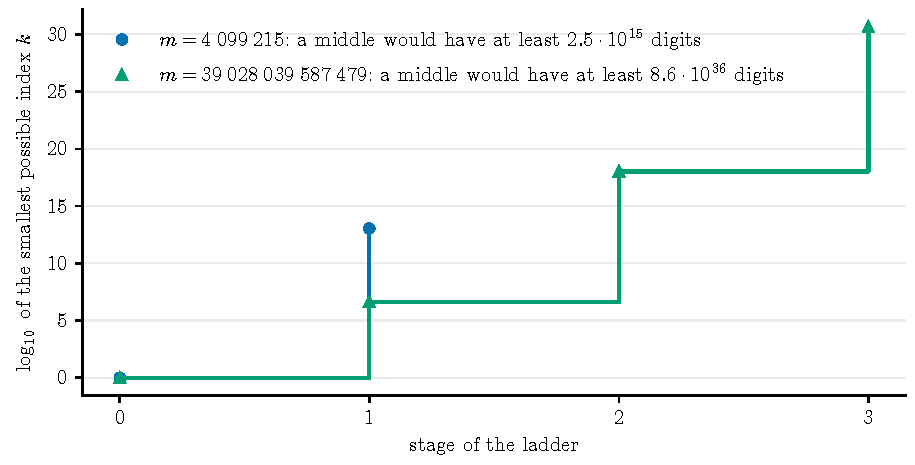
\includegraphics[width=\textwidth]{fig_leiter}
\caption{\textbf{Each stage of a ladder pushes the smallest possible index up.} The ladder of Table~\ref{tab:reinhart}, stage by stage. Each step multiplies the smallest possible index $k$ by the product of
the witnesses of that stage; the last point is the smallest index that remains possible.}\label{fig:leiter}
\end{figure}

\begin{proof}[How the table is computed]
Let $k_0$ be an index with $v_p(T_{k_0}) = 1$ for an odd prime $p$, and let $T_k$ be powerful with $k_0 \mid k$ and $k/k_0$ odd. By
Lemma~\tref{lem:bewertung}, $v_p(T_k) = 1 + v_p(k/k_0) \ge 2$, so $p \mid k/k_0$. Starting at $k_0 = 1$, the product of the witnesses of a
stage therefore divides $k/k_0$, and the next stage starts at $k_0$ times that product. The witnesses are found from $T_1$ and $U_1$
modulo $p^2$, without large integers. The ladder stops at the first stage without a witness below $P$.
\end{proof}

\inwords These two kernels are dangerous in the sense of Section~\tref{sec:hoehe}, because they divide $U_1$; the other two known kernels divide $U_1$ as well, but their $T_1$ is odd. For each of them the table
shows how far out a triple would have to be: the middle would have at least the number of digits in the last column. For
$m = 4\,099\,215$ the indices $k = \Z{reinhartboxk}$ also lie in the box of Theorem~\tref{thm:reduktion}, where they are excluded by the
witnesses \Z{reinhartboxz}.

Reinhart \cite[Def.~1.4, p.~6]{Reinhart2024} asks whether $4\,099\,215$ or $39\,028\,039\,587\,479$, or even $7$, admits an index $k$ with
$T_k$ powerful and $m \mid U_k$ (his condition (C), Question~\tref{q:reinhart}). Our first witnesses $\Z{reinhartza}$ and $\Z{reinhartzc}$ for these two kernels are
his own. The table does not decide the question; it only says how large a positive answer would have to be.

\begin{proposition}[the smallest witnesses]\tlabel{prop:zeugen}\belegart{computed}
For each of the \Z{zeugenalle} lattice points of Theorem~\tref{thm:reduktion} that are excluded by a witness, let $p$ be the smallest
witness and $\alpha_m(p)$ its rank. In \Z{zeugenprim} points the smallest witness is primitive, $\alpha_m(p) = k$; in all others it is a
prime whose rank divides $k$ with odd cofactor. The smallest witness is $29$ in \Z{zeugen29} points, $19$ in \Z{zeugen19}, $11$ in
\Z{zeugen11}, $3$ in \Z{zeugen3}, $5$ in \Z{zeugen5} and $7$ in \Z{zeugen7}; its median is \Z{zeugenmedian} and its maximum
\Z{zeugenmax}. In every point $v_p(T_{\alpha_m(p)}) = 1$ and $p \nmid k/\alpha_m(p)$.
\end{proposition}

The valuation identity of Lemma~\tref{lem:bewertung} was checked in every point. As controls, the point $(\Z{beispielm}, \Z{beispielk})$ has the witness $\Z{beispielzeuge}$ of
rank $\Z{beispielk}$, and the identity predicts $v_{\Z{zeugennkp}}(T_{\Z{zeugennkk}}(7)) = \Z{zeugennkv}$, which the exact computation confirms.

\inwords A triple would have to survive the test of Theorem~\tref{thm:zeugen} not only at the primes that first appear at its index
$k$, but at every small prime whose rank divides $k$. In practice the lattice points fail at small primes: the typical witness is
$19$ or $29$, and only at \Z{zeugenprim} of the points is the smallest witness a prime that first appears at $k$ itself.

\begin{remark}[the condition modulo $36$ and the witnesses]\tlabel{rem:rizzi}\belegart{computed}
By Beckon's condition (Remark~\tref{rem:kongruenzen}) the middle $n$ of a triple satisfies $n \equiv 0$, $8$ or $28 \pmod{36}$; the earliest
derivation we located is Beckon's \cite[Theorem~0.1]{Beckon2019}. Proposition~3(i) of \cite{Sayim2026EMW} refines it to $39$ classes modulo $900$ and
$1209$ classes modulo $44\,100$. Rizzi \cite[Proposition~5.1]{Rizzi2026} derives the condition modulo $36$ again and notes that it agrees with Beckon's; the same
paper reports a search up to $10^{10}$ that finds fourteen pairs and no triple \cite[Chapters~4 and~6]{Rizzi2026}. Of the \Z{zeugenalle} middles of Proposition~\tref{prop:zeugen}, \Z{rizzierfuellt} satisfy the
condition, and the \Z{rizzinicht} that do not are exactly the points whose smallest witness is $3$.
\end{remark}

This is no coincidence. For the middle $n$ of a pair, that is, with $n - 1$ and $n + 1$ powerful, and $4 \mid n$, the condition fails exactly when $n$ is
divisible by $3$ but not by $9$, that is, when
$v_3(T_k) = 1$; then $3$ is a witness, and the smallest one. So the condition modulo $36$ is the case $p = 3$ of the witness reduction.
Since the two computations work by different methods, their agreement on the same points checks both.

\inwords A known rule says what the middle of a triple must look like modulo $36$. Our witness search already contains this rule: the
middles that break it are exactly those where the prime $3$ appears only once.

\begin{proposition}[how many conditions there are, and how often they are met]\tlabel{prop:teilerdaten}\belegart{computed}
\begin{enumerate}
\item[(a)] For the \Z{kongrkerne} kernels of class $7$ with the most lattice points and all primes $p \le \Z{kongrp}$ that have a rank $d$,
  the congruence $p \equiv \pm 1 \pmod{4d}$ of Corollary~\tref{cor:teiler}(i) holds at all \Z{kongrpaare} pairs $(p, d)$.
\item[(b)] Over the \Z{bedpunkte} lattice points of Theorem~\tref{thm:reduktion}, the indices $k$ have \Z{bedteiler} divisors $d \ge 5$ in
  total (median \Z{bedallemedian} per point, maximum \Z{bedallemax}). For \Z{bedausweg} of them (\Z{bedanteil}\,\%) one has $k < d(4d - 1)$,
  so by Corollary~\tref{cor:teiler}(iii) a powerful $T_k$ would need $p_d^2 \mid T_d$ at that $d$. Per point the number of such
  conditions has median \Z{bedmedian}, mean \Z{bedmittel} and maximum \Z{bedmax}.
\item[(c)] For the \Z{beskerne} kernels of class $7$ with the most lattice points (\Z{bespunkte} points), every divisor of every $k$ was
  taken as a rank, and for each rank the first \Z{besnp} primes of that rank below $\Z{besp}$ were tested. Of the \Z{besraenge} rank occurrences (a point together with a divisor of its index, so that $d = 1$ and $d = 3$ are included and one pair $(m, d)$ counts once for every
  point whose index $d$ divides), \Z{besbesetzt} have a prime below this bound, and \Z{beszeuge} of these (\Z{beszeugeant}\,\%) carry a witness; \Z{beswief} carry only
  primes with exponent at least $2$. Testing only the smallest prime of each rank gives \Z{beseinszeuge} of the same \Z{besbesetzt}
  ranks (\Z{beseinsant}\,\%) and \Z{beseinswief} with exponent at least $2$ only.
\end{enumerate}
\end{proposition}

The \Z{besleer} rank occurrences without a prime below the bound are undecided; for $d \ge 5$ they are not known to be free of witnesses, since their smallest prime lies
higher, and among them are the occurrences of $d = 1$ at kernels with $T_1(m)$ a power of $2$, which have no odd prime at all. Parts (b)
and (c) report rates. No proof in this paper depends on them, and Corollary~\tref{cor:teiler} holds independently of them; the single
ranks behind (c) are decided, since one prime of exponent $1$ settles its rank by Theorem~\tref{thm:zeugen}.

\inwords Part (a) checks a proved rule on \Z{kongrpaare} cases. Part (b) counts how many separate tests a triple would have
to pass at a lattice point: typically a few, sometimes a dozen. Part (c) shows how often such a test is actually decided by a small prime:
almost always, and more often when more primes per rank are tried.

\begin{proposition}[middles that are powers of two]\tlabel{prop:zweierpotenz}\belegart{computed}
For every integer $a$ with $2 \le a \le \Z{zweiamax}$, at least one of $2^a - 1$ and $2^a + 1$ is not powerful. In particular no triple has
a middle $2^a$ in this range, that is, a middle of this form with up to \Z{zweistellen} digits.
\end{proposition}

\begin{proof}[The computation]
For each prime $p \le \Z{zweip}$ let $e$ be the order of $2$ modulo $p$. The prime $p$ divides $2^a - 1$ exactly when $e \mid a$, and then
$v_p(2^a - 1) = v_p(2^e - 1) + v_p(a/e)$; so $p$ is a witness for $2^a - 1$ exactly when $e \mid a$, $p^2 \nmid 2^e - 1$ and $p \nmid a/e$.
The prime $p$ divides $2^a + 1$ exactly when $e$ is even and $a$ is an odd multiple of $e/2$, and then $v_p(2^a + 1) = v_p(2^{e/2} + 1) + v_p(2a/e)$; so $p$ is a witness for
$2^a + 1$ exactly when $e$ is even, $a$ is an odd multiple of $e/2$, $p^2 \nmid 2^{e/2} + 1$ and $p \nmid 2a/e$. The loop runs over the
primes rather than over the exponents. Among the \Z{zweiexp} exponents, \Z{zweiminus} (\Z{zweiminusant}\,\%) leave $2^a - 1$ without a
witness below the bound and \Z{zweiplus} (\Z{zweiplusant}\,\%) leave $2^a + 1$ without one; no exponent leaves both without one.
\end{proof}

The exponents without a witness are undecided; they are not known to be powerful: their prime factors lie above the search bound. Equivalently, $2^a - 1$ is
proved not powerful for \Z{zweiminusok} of the exponents and $2^a + 1$ for \Z{zweiplusok}. As controls, the computation of the orders
returns exactly the two Wieferich primes $1093$ and $3511$ below the bound, and $2^3 + 1 = 9$, which is powerful, receives no witness.
Question~\tref{q:zweierpotenz} asks for all $a$.

\inwords If the middle of a triple were a power of two, then $2^a - 1$ and $2^a + 1$ would both be powerful. For every $a$ up to
\Z{zweiamax} a small prime appears exactly once in one of the two numbers. The search runs over primes, which makes it cheap.

%
\begin{figure}[tp]
\centering
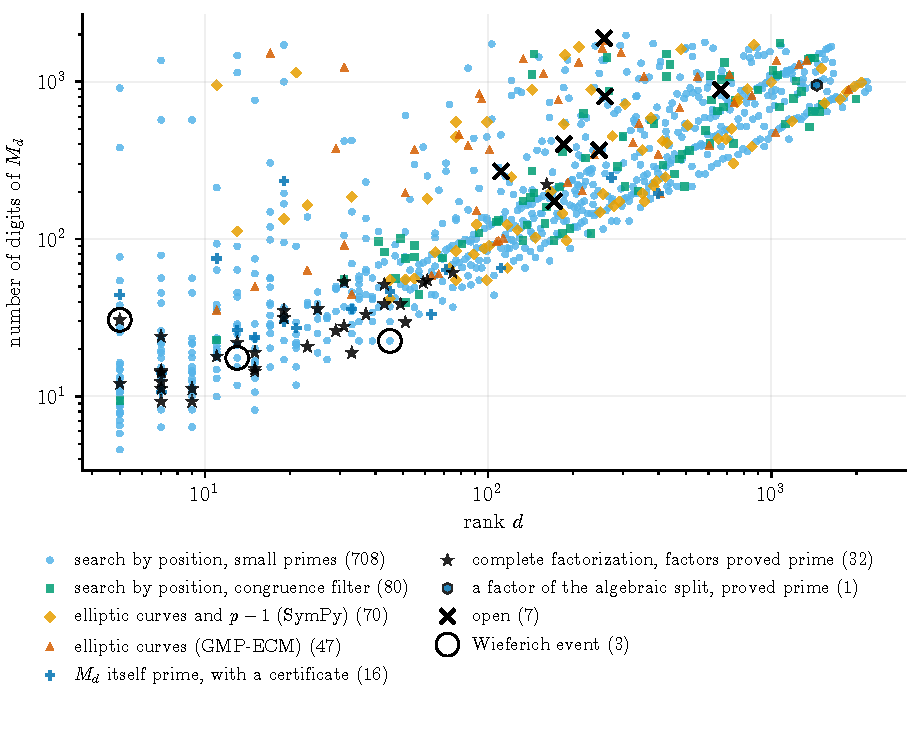
\includegraphics[width=\textwidth]{fig_karte}
\caption{\textbf{Every building block, settled or open.} The \Z{rgpaare} building blocks $\Prim{d}$ of Proposition~\tref{prop:raenge}, one point each: the rank $d$ against the number
of digits, both on logarithmic scales. Color and shape show how each block was shown not to be powerful; the classes are the rows of
Table~\ref{tab:wege}, and every class except the open blocks is a certified witness. The \Z{rgoffen} open blocks (crosses) have at least \Z{offenmin} digits
each, and no search found a factor of them. Circles mark the \Z{wfinpop} blocks with a Wieferich event below $\Z{wfp}$
(Proposition~\tref{prop:lucaswieferich}). The terms are explained in Table~\ref{tab:legende}.}\label{fig:karte}
\end{figure}

\begin{proposition}[the primitive part over an explicit finite set]\tlabel{prop:raenge}\belegart{computed}
Let $\mathcal{P}$ be the set of the \Z{punkte} lattice points of Theorem~\tref{thm:reduktion}; all of them are excluded there. For a
kernel $m$ of a point of $\mathcal{P}$ and an odd $d \ge 5$ dividing an index $k$ with $(m, k) \in \mathcal{P}$, let $\Prim{d}$ be the part of
$T_d(m)$ supported on the primes of rank exactly $d$. There are \Z{rgpaare} such pairs $(m, d)$, on the \Z{rgkerne} kernels of $\mathcal{P}$.
\begin{enumerate}
\item[(a)] \emph{Settled: \Z{rgerledigt} of the \Z{rgpaare}, each by a certified witness.}
\item[(b)] \emph{Open: \Z{rgoffen} of the \Z{rgpaare}.}
\end{enumerate}
\end{proposition}

A witness here is a prime $p$ of rank $d$ with $v_p(\Prim{d}) = 1$; it shows that $\Prim{d}$ is not powerful. For some blocks the witness
comes from a complete factorization, and for one from the algebraic split of Remark~\tref{rem:zweiprimitive}. For a prime $p$ of rank exactly $d$ one has $v_p(\Prim{d}) = v_p(T_d)$ by definition; for the Möbius dual
$\prod_{e \mid d} T_e^{\mu(d/e)}$, the product with which the computations work, the same holds at every prime of rank exactly $d$
\cite[Theorem~2.2(c)]{RossShenCai2026}; the restriction to odd $d$ is the range in which the dual of the
companion sequence is integral \cite[Theorem~2.3]{RossShenCai2026}. Since every point of $\mathcal{P}$ is already excluded, the
proposition excludes no further triple. It asks, on these pairs, whether a primitive part can be powerful
(Question~\tref{q:primindex}). For \Z{rgungerade} of the kernels $T_1(m)$ is odd; their points are excluded by parity alone and enter only
as instances of that question.

\begin{table}[ht]
\centering
\small
\begin{tabular}{lrrr}
\hline
how the pair was settled & first \Z{rgaltkerne} kernels & other \Z{rgneukerne} & all \\
\hline
\Z{wegetab}
\hline
\end{tabular}
\caption{How the \Z{rgpaare} pairs of Proposition~\tref{prop:raenge} were settled. The first \Z{rgaltkerne} kernels are those with the most
lattice points; for the other \Z{rgneukerne}, and for the pairs of the first \Z{rgaltkerne} with $t_{35} < 1$, the elliptic curve method ran to a smaller effort, see Table~\ref{tab:offen}.}\label{tab:wege}
\end{table}

\begin{proof}[How the pairs were settled]
\emph{A search by position.} Every prime $p \le \Z{erstesucheP}$ of rank $d$ was tested, and later, restricted by
Corollary~\tref{cor:teiler}(i) to $p \equiv \pm 1 \pmod{4d}$, every such prime up to $\Z{siebober}$. For the pairs that remain open, this search also shows that no prime of
rank $d$ with $v_p(\Prim{d}) = 1$ lies below its bound.
\emph{A search by size.} The elliptic curve method, first with SymPy \cite{Meurer2017} and then with GMP-ECM \cite{GMPECM706}, looks
for a factor by its size rather than by its position; it shows only what it finds. The effort spent on the pairs that remain open is in
Table~\ref{tab:offen}.
\emph{Complete factorization.} Small primitive parts were factored completely, and some are themselves prime, which no
search for a proper divisor can see. One pair, $(m, d) = (319, 5)$, has no witness below the first bound and
has its own row in Table~\ref{tab:wege}; its witnesses come from the complete factorization of $\Prim{5}(319)$ given after Proposition~\tref{prop:lucaswieferich}, whose large
factors are proved prime.
\emph{Checks.} Every witness was recomputed on a second, independent route (the powers of $\varepsilon_m$ with the rank taken from the
order of the unit, or the Lucas sequence $V_n(2T_1, 1)$, whichever differs from the route that found it). Every witness of the \Z{rgzert} pairs in the first part of (a) is
certified: below $\psi_{12}$ by the Miller--Rabin test with the first twelve prime bases, which is deterministic there
\cite{SorensonWebster2017}, and above it by Pocklington's criterion from a factorization of $p - 1$ \cite[Theorem~4 and Corollary~1]{BrillhartLehmerSelfridge1975},
each certificate checked by a separate program. The prime factors of the complete factorizations and the factor from the algebraic
split are certified in the same way: below $\psi_{12}$ by the deterministic test, and above it \Z{pbpock} of them, with up to
\Z{pbpockmax} digits, by Pocklington's criterion, and \Z{pbecpp}, with up to \Z{pbecppmax} digits, by elliptic curve certificates
\cite{GoldwasserKilian1986,AtkinMorain1993}, which PARI/GP \cite{PARI2172} produced and a separate program of ours checked step by step.
\end{proof}

\begin{table}[ht]
\centering
\small
\begin{tabular}{rrrrrrrr}
\hline
$m$ & $d$ & digits & \multicolumn{3}{c}{curves at $B_1 =$} & $t_{35}$ & $t_{40}$ \\
 & & & $5\cdot 10^4$ & $10^6$ & $3\cdot 10^6$ & & \\
\hline
\Z{offentab}
\hline
\end{tabular}
\caption{The \Z{rgoffen} open pairs of Proposition~\tref{prop:raenge} and the effort of GMP-ECM on each. The columns $t_{35}$ and $t_{40}$
give the fraction of the curves the program expects to need for a factor of $35$ and of $40$ digits, for the second-stage bound it chose.
A fraction of $1$ still misses a factor of that size with probability about $1/e$, so ``none found'' describes the effort, not the
factors. The kernels \Z{offenneum} are among the other \Z{rgneukerne}; the rest are among the first \Z{rgaltkerne}. The blocks that the searches left open on the kernels $m = \Z{teilezeugem}$ and $m = \Z{teilevollm}$, where $T_1(m) + 1$ is a
square, are settled by the algebraic split of Remark~\tref{rem:zweiprimitive} and are not listed.}\label{tab:offen}
\end{table}

\inwords Theorem~\tref{thm:reduktion} already rules out all \Z{punkte} lattice points in its search range. This proposition asks a
different question: can a building block $\Prim{d}$ be powerful at all? We take all \Z{rgkerne} kernels of the lattice points and look at
every building block that occurs there, \Z{rgpaare} in total. A number is powerful when each of its prime factors appears at least twice.
So one prime that appears exactly once is enough to show that a block is not powerful. We found such a prime, and proved that it is
prime, for \Z{rgzert} blocks; for some of them we split the whole block into its prime factors, and for one the algebraic split of
Remark~\tref{rem:zweiprimitive} gives the factor. Every prime used is proved prime, the large ones by certificates that our own program
checks. For the last \Z{rgoffen} blocks we found no such prime. Finding nothing only means that
our search did not succeed, not that no such prime exists.
The \Z{rgoffen} open blocks are in the deposit with their decimal expansions; a prime factor of any one of them with exponent one settles
that block, and a complete factorization settles it either way.

\emph{A different question, measured.} Among the \Z{prtripel} triples $(m, d, p)$ of the search by position with $p \le \Z{erstesucheP}$
(for each rank, the first five primes found by the search), $v_p = 1$ in \Z{prvauf1} cases, $v_p = 2$ in \Z{prvauf2} and $v_p \ge 3$ in none. The heuristic
$P(v_p \ge j) = p^{1-j}$ predicts \Z{prerwartet} triples with $v_p \ge 2$. The observations are consistent with it and do not confirm it.

\begin{remark}[where this stands in the literature]\tlabel{rem:literatur}\belegart{literature}
Ribenboim and Walsh \cite[Corollary~2]{RibenboimWalsh1999} show that the abc conjecture implies that a Lucas sequence of positive discriminant has only
finitely many powerful terms, and Yabuta \cite{Yabuta2007} extends this to negative discriminant. These statements concern the terms rather
than their primitive parts, and they are conditional and not effective, so they neither contain nor are contained in the computation
above. Closer to the question is \cite[Corollary~5.1]{RossShenCai2026}: the primitive parts of the Fibonacci numbers are squarefree for all
$n \ne 6$ if and only if there is no Wall--Sun--Sun prime. Squarefree is a far stronger property than not powerful; the question asked here
is the weaker one, and it is the one a finite computation can address.
\end{remark}

\inwords If the $abc$ conjecture is true, only finitely many terms of such sequences are powerful, but nobody knows which, and the
statement is about whole terms, not their building blocks. For the Fibonacci numbers, even the question whether all building blocks are
squarefree is tied to an open problem about special primes.

\begin{proposition}[Wieferich primes of the unit and the primitive parts]\tlabel{prop:lucaswieferich}\belegart{proved}
Fix a squarefree $m \equiv 7 \pmod 8$ with $T_1(m)$ even. For odd $d \ge 5$ let $\Prim{d}$ be the part of $T_d(m)$ supported on the
primes of rank exactly $d$. Call an odd prime $p \nmid m$ that divides some $T_k(m)$ a \emph{Wieferich prime for $\varepsilon_m$} if
$p^2 \mid T_{\alpha_m(p)}(m)$. The following are equivalent:
\begin{enumerate}
\item[(i)] $\varepsilon_m$ has only finitely many Wieferich primes of odd rank;
\item[(ii)] $\Prim{d}$ is squarefree for all but finitely many odd $d \ge 5$.
\end{enumerate}
In that case $\Prim{d}$ is not powerful for all but finitely many odd $d \ge 5$. Moreover, let $p \nmid m$ be an odd prime that has a rank $\alpha$, let
$u_n = U_n/U_1$ be the Lucas sequence of the first kind for $(P, Q) = (2T_1, 1)$, and let $e = (m/p)$. Then $p \nmid U_1$ and $v_p(u_{p - e}) = v_p(T_\alpha)$.
So the Wieferich primes for $\varepsilon_m$ are exactly the odd Lucas--Wieferich primes of this sequence that divide some $T_k$.
\end{proposition}

\begin{proof}
A prime $p$ dividing $\Prim{d}$ has rank exactly $d$, so $v_p(\Prim{d}) = v_p(T_d) = v_p(T_{\alpha_m(p)})$; in the language of Möbius duals
this is \cite[Theorem~2.2(c)]{RossShenCai2026}. Hence $p$ divides $\Prim{d}$ exactly once when $p$ is not a Wieferich prime for
$\varepsilon_m$. (i) $\Rightarrow$ (ii): a Wieferich prime of odd rank $d$ affects only $\Prim{d}$, so under (i) all $\Prim{d}$ outside
finitely many odd $d$ are squarefree. (ii) $\Rightarrow$ (i): a Wieferich prime of odd rank $d \ge 5$ makes $\Prim{d}$ non-squarefree, so
under (ii) such primes have one of finitely many ranks, and each rank carries finitely many primes, since $\Prim{d}$ is a positive
integer; the ranks $1$ and $3$ carry only the prime divisors of $T_1$ and $T_3$. For the last assertion, $\Prim{d} > 1$ for odd $d \ge 5$,
because $T_d$ has a primitive prime divisor \cite{Carmichael1913}, in the form of \cite{Yabuta2001} used in the proof of
Corollary~\tref{cor:teiler}; and a squarefree integer above $1$ is not powerful.
For the last statement, $p \mid T_\alpha$ gives $\varepsilon_m^{2\alpha} + 1 = 2\varepsilon_m^{\alpha} T_\alpha \equiv 0 \pmod p$ in $\mathbb{Z}[\sqrt{m}]$, and the proof of
Corollary~\tref{cor:teiler}(i) shows that $\varepsilon_m$ has order $4\alpha$ modulo the primes above $p$ and that $4\alpha \mid p - e$; in particular $p \nmid U_1$, because
$p \mid U_1$ would give $\varepsilon_m^2 \equiv 1$. Write $y = \varepsilon_m^{4\alpha}$ and $M = (p - e)/(2\alpha)$, so that $\varepsilon_m^{2(p-e)} = y^M$ and
$y \equiv 1 \pmod p$. Here $p \nmid M$, because $p \nmid p - e$, and $y^M - 1 = (y - 1)(1 + y + \dots + y^{M-1})$ with the second factor congruent to $M$ modulo $p$.
Multiplication by an element of $\mathbb{Z}[\sqrt{m}]$ whose norm is prime to $p$ does not change $v_p$ (see the proof of Lemma~\tref{lem:bewertung}), so
$v_p(y^M - 1) = v_p(y - 1)$. Next, $y - 1 = (\varepsilon_m^{2\alpha} + 1)(\varepsilon_m^{2\alpha} - 1)$ with $\varepsilon_m^{2\alpha} - 1 \equiv -2 \pmod p$ of norm prime to $p$, so
$v_p(y - 1) = v_p(2\varepsilon_m^{\alpha} T_\alpha) = v_p(T_\alpha)$. Finally $\varepsilon_m^{p-e} \cdot u_{p-e} \cdot 2U_1\sqrt{m} = \varepsilon_m^{2(p-e)} - 1$, and the norms of
$\varepsilon_m^{p-e}$ and $2U_1\sqrt{m}$ are prime to $p$, so $v_p(u_{p-e}) = v_p(\varepsilon_m^{2(p-e)} - 1) = v_p(T_\alpha)$.
\end{proof}

\inwords A prime $p$ is a Wieferich prime (to base $2$) if $p^2$ divides $2^{p-1} - 1$. Below $\Z{zweip}$ there are exactly two, $1093$
and $3511$ (the control in Proposition~\tref{prop:zweierpotenz}). Fix one $m$ with $T_1(m)$ even. The rank of a prime $p$ is the first $k$
with $p$ dividing $T_k(m)$. We call $p$ a Wieferich prime for $m$ if $p^2$ already divides the term at its rank. If this rank $d$ is odd and
at least $5$, then $p^2$ divides the block $\Prim{d}$, so $\Prim{d}$ is not squarefree. Proposition~\tref{prop:lucaswieferich} says: the
blocks $\Prim{d}$ with odd $d$ are squarefree from some point on exactly when only finitely many such primes have odd rank. In that case
only finitely many blocks with odd $d$ can be powerful. Such primes do exist. Among the primes below $\Z{wfp}$ we found \Z{wfgerade} of odd
rank $d \ge 5$ on those of the \Z{wfkerne} kernels of Proposition~\tref{prop:raenge} that have $T_1$ even. Since finitely many are allowed, these do not
settle the condition. For \Z{wfentschieden} of them the block is not powerful: another prime divides it exactly once. For the other
\Z{wfoffen} we do not know. Whether a block can be powerful remains open in general. For the Fibonacci numbers, the same kind of
condition is the open question whether a Wall--Sun--Sun prime exists.

For the Fibonacci numbers, Ross, Shen and Cai show that the M\"obius duals $\prod_{d \mid n} F_d^{\mu(n/d)}$ are squarefree for all $n \ne 6$ exactly when there is no
Wall--Sun--Sun prime \cite[Corollary~5.1]{RossShenCai2026}. The proposition is the analog for $\varepsilon_m$, restricted to odd rank
and allowing finitely many exceptions; it is elementary, and its content is the identification of the hypothesis.

\begin{remark}[the Wieferich events of the units]\tlabel{rem:wfdaten}\belegart{computed}
That hypothesis is not empty for our units. Among the primes below $\Z{wfp}$ the \Z{wfkerne} units of Proposition~\tref{prop:raenge} carry \Z{wfereignisse} Wieferich
events, that is, pairs of a unit and a prime (\Z{wfprimzahlen} distinct primes). Of these, \Z{wfungerade} have odd rank $d \ge 5$, and
\Z{wfgerade} of those lie on units with $T_1$ even, where the proposition applies; Table~\ref{tab:wieferich} lists them. So the squarefree
statement for all odd $d$ fails for these units. In \Z{wfzeuge} of the \Z{wfgerade} cases $\Prim{d}$ is nevertheless not powerful, since a
prime of rank $d$ below $\Z{wfp}$ divides it exactly once, and $\Prim{5}(319) = \Z{wfmquadrat}^2 \cdot \Z{wfmgross} \cdot \Z{wfmgroesser}$ with both
large factors proved prime. For the remaining \Z{wfoffen} the question is not settled here; they lie outside the finite set of
Proposition~\tref{prop:raenge}. Conversely, the \Z{wfinpopzu} events whose block lies in that set, the circles in Figure~\ref{fig:karte}, are all
settled; the last column of Table~\ref{tab:wieferich} marks them. On the \Z{erstesuchekerne} units of the first search there are
\Z{wfnullrang} events. Part~III finds more on the same units (Remark~\partref{III}{rem:wieferichbrueche}) because it also counts primes
that divide no $T_k(m)$. Whether a primitive part can be powerful at all is Question~\tref{q:primindex}.
\end{remark}

\begin{table}[ht]
\centering
\begin{tabular}{rrrll}
\hline
unit $m$ & rank $d$ & prime $p$ & $\Prim{d}$ not powerful by & in Prop.~\tref{prop:raenge} \\
\hline
\Z{wftab}
\hline
\end{tabular}
\caption{The Wieferich events of odd rank $d \ge 5$ below $\Z{wfp}$ on the units $\varepsilon_m$ of Proposition~\tref{prop:raenge} with $T_1(m)$ even. ``Witness'': a
prime of rank $d$ below $\Z{wfp}$ divides $\Prim{d}$ exactly once. ``Not settled'': not decided by our computations. The last column says
whether $(m, d)$ is one of the \Z{rgpaare} pairs of Proposition~\tref{prop:raenge}.}\label{tab:wieferich}
\end{table}

\begin{remark}[Lucas--Wieferich primes]\tlabel{rem:lucaswf}\belegart{computed}
The condition in (i) has a name in the computational literature. For the Lucas sequence $(u_n)$ of the first kind attached to $(P, Q) = (2T_1, 1)$,
a prime $p$ with $u_{p - e} \equiv 0 \pmod{p^2}$, where $e$ is the Legendre symbol of the discriminant, is a Lucas--Wieferich prime
\cite[p.~2088]{McIntoshRoettger2007}. That condition is placed on the sequence of the first kind and ours on the companion sequence, but for primes that have a rank the
two agree, by the last statement of Proposition~\tref{prop:lucaswieferich}. The computation agrees as well: on the \Z{lucasgleich} events of the first search of Proposition~\tref{prop:raenge} (the \Z{erstesuchekerne}
units with the most lattice points) the two conditions select the same primes; as controls, the \Z{lucaspk} Wieferich primes $\Z{pellwief}$ of the Pell
sequence are recognized, and \Z{lucasnk} primes that divide their term exactly once are not. This checks the computation on one sequence; the
identity itself is proved above.
\end{remark}

\begin{remark}[a second primitive prime factor]\tlabel{rem:zweiprimitive}\belegart{computed}
If every block $\Prim{d}$ with $d \ge 5$ had two distinct prime factors, a powerful block would need two primes of rank $d$ that each divide
$T_d(m)$ at least twice, two simultaneous events of the kind counted in Proposition~\tref{prop:exponenten}. For Lehmer numbers there is a
theorem of this kind: Juri\v{c}evi\'{c} \cite[Theorems~1.1 and~2.1]{Juricevic2007}, making a result of Schinzel effective, proves that the $n$-th
term of a real Lehmer pair has at least two primitive prime divisors when $n > 4$, $n \ne 6$ and $n/(\eta\kappa)$ is odd, where $\eta$ and $\kappa$ are
invariants of the pair, apart from an explicit list of exceptions with $n \le 30$. Here $\Prim{d}$ is the primitive part of the term of index $2d$ of the Lucas sequence $u_n(2T_1, 1) =
U_n/U_1$, whose terms of even index are $2T_1$ times the Lehmer numbers of the pair with $L = 4T_1^2$ and $M = 1$. For this pair
$\eta = \kappa = 1$, so the condition asks for $2d$ to be odd, and the theorem does not apply to any block.

\emph{A second pair.} If $T_1(m) + 1 = x^2$ is a square, then $\varepsilon = \gamma^2$ with $\gamma + \gamma^{-1} = x\sqrt{2}$, and $(\gamma, \gamma^{-1})$ is a
real Lehmer pair with $L = 2x^2$ and $M = 1$, for which $\kappa = 2$ and $\eta = 2$. Its term of index $4d$ is the term of index $2d$ above, so its
primitive divisors are the primes of rank $d$, and for odd $d \ge 5$ the quotient $4d/(\eta\kappa) = d$ is odd; none of the exceptional triples has
these values. Hence on such a kernel every block $\Prim{d}$ with $d \ge 5$ has at least two distinct prime factors. The split behind it is elementary: for odd $d$,
$T_d + 1 = (x w_d)^2$ with $w_d = (\gamma^d + \gamma^{-d})/(\gamma + \gamma^{-1})$ an integer, so $T_d = (s - 1)(s + 1)$ with $s = x w_d$, and
the odd number $\Prim{d}$ is the product of the coprime factors $\gcd(\Prim{d}, s - 1)$ and $\gcd(\Prim{d}, s + 1)$; that $\Prim{d}$ has two
distinct prime factors is the content of the theorem. This is a splitting of the same kind as the Aurifeuillian factorization of the Lucas numbers,
where the primitive part of $L_{5n}$, for odd $n$, is the product of two coprime factors \cite[(2.9)--(2.11)]{BrillhartMontgomerySilverman1988}.
The case occurs
for \Z{zquadkerne} of the \Z{rgkerne} kernels of Proposition~\tref{prop:raenge}, which carry \Z{zquadbl} of the \Z{rgpaare} blocks, and for every prime kernel
$m \equiv 7 \pmod 8$: the class number is odd, so $x^2 - m y^2 = 2$ is solvable (Remark~\tref{rem:aussen} gives an elementary proof), and we checked it for the \Z{zquadprim} prime kernels below \Z{zquadgrenze}.
We also checked the conclusion on each of these \Z{zquadbl} blocks: $\Prim{d}$ is composite and not a prime power.

On the other kernels the theorem does not apply, and the data show that a block can have a single prime factor: of \Z{zpn} blocks $\Prim{d}$ with $d \ge 5$
and small $T_d(m)$ that we factored completely, \Z{zpprim} are prime, none of them on a kernel of the kind above, the largest at $d = \Z{zpdmax}$, and
\Z{zpab16} of these have $2d \ge 31$, so that it is the parity condition and not the size of $n$ that fails. So on the \Z{zquadkerne} kernels a
powerful block needs two rare events, and on the others no argument of this kind forces two events: a block can have a single prime factor, and a powerful
block could then be the power of a single prime.

The split also settles blocks that the searches of Proposition~\tref{prop:raenge} left open. For $(m, d) = (\Z{teilevollm}, \Z{teilevolld})$
both factors $\gcd(\Prim{d}, s - 1)$ and $\gcd(\Prim{d}, s + 1)$, with \Z{teilevolla} and \Z{teilevollb} digits, are prime, so
$\Prim{d}$ is their product and is not powerful. For $(m, d) = (\Z{teilezeugem}, \Z{teilezeuged})$ one factor, with
\Z{teilezeugest} digits, is prime; since the two factors are coprime, it divides $\Prim{d}$ exactly once. All three primes are proved by
elliptic curve certificates (proof of Proposition~\tref{prop:raenge}).
\end{remark}

\inwords One could hope that a building block always has at least two different primes, so that a powerful block would need two rare
events at once. A theorem of this type exists for a related sequence. On the kernels for which $T_1 + 1$ is a square, it applies after a change of the
sequence, and there every block has at least two primes. On the other kernels its condition is never met by our blocks, and in our data some
blocks are themselves prime. So there one rare event may be all that a powerful block needs.

\section{Profile of a counterexample}\tlabel{sec:profil}

This section collects in one place what is known about a triple, if one exists. Every clause is proved above or computed in
Section~\tref{sec:gebiete} or~\tref{sec:daten}, and the clauses that depend on Reinhart's extended search say so; nothing new is claimed here except clause~(viii).

%
\begin{theorem}[profile]\tlabel{thm:profil}\belegart{computed}
Suppose that $n - 1$, $n$ and $n + 1$ are all powerful, let $m = \operatorname{sqfree}(n^2 - 1)$, and let $(m, k)$ be the address of $n$.
\begin{enumerate}
  \item[(i)] $m \equiv 7 \pmod 8$ is squarefree, $T_1(m)$ is even, $k$ is an odd multiple of $m'$, $n = T_k(m)$, and $4 \mid n$.
  \item[(ii)] $n \ge (m^{3/2}/m')^{m'}$. If $m \nmid U_1$, then $n > m^{9/2}/27$ and $k \ge 3$; if $m \mid U_1$, then $n \ge T_1 > m^{3/2}$.
  \item[(iii)] $v_2(n) = v_2(T_1(m))$, and $k$ is divisible by every odd prime $p$ with $v_p(T_1(m)) = 1$.
  \item[(iv)] Every odd prime $p \mid n$ is coprime to $m$, $k$ is an odd multiple of $\alpha_m(p)$, and
  $v_p(T_{\alpha_m(p)}) + v_p(k/\alpha_m(p)) \ge 2$. Every prime $p$ with $\alpha_m(p) = k$ satisfies $p^2 \mid n$.
  \item[(v)] Let $b = \operatorname{sqfree}(n)$. If $b > 1$, then $k = \alpha_m(b)$, and
  $v_p(T_{\alpha_m(p)}) + v_p(\alpha_m(b)/\alpha_m(p)) \ge 3$ for every odd prime $p \mid b$.
  \item[(vi)] If $n$ is a square, twice a square, or a fourth power, then $k = 1$, $m \mid U_1$, and $m > 1.5 \cdot 10^{12}$ or $m$ is one of
  $209\,991$, $4\,099\,215$ and $117\,477\,414\,815$, which carry no triple with such a middle; if Reinhart's extended search missed nothing
  (Remark~\tref{rem:reinhartliste}), then $m > 5.325 \cdot 10^{13}$ or $m$ is one of the four known values.
  \item[(vii)] Explicit exclusions. Either $m > \Z{kernschranke}$ or $n \ge 10^{\Z{hoehe}}$. If $m \le \Z{bboxkern}$, then
  $\operatorname{sqfree}(n) > \Z{bboxb}$. If $m \le \Z{streifenschranke}$, then $n$ has more than $\Z{streifenstellen}$ digits. If
  $\Z{glattunten} < m \le \Z{glattoben}$ and $m$ is a product of at least $\Z{glattmin}$ primes up to $\Z{glattprim}$, then
  $n \ge 10^{\Z{glatthoehe}}$. If $m \mid U_1$ and $m \le 1.5 \cdot 10^{12}$, then $m = 4\,099\,215$, which
  forces $k \ge \Z{turmk1}$ (the other members of Reinhart's list below this bound, $209\,991$ and $117\,477\,414\,815$, have $T_1$ odd and carry no
  triple); if Reinhart's extended search missed nothing, the same holds for
  $m \le 5.325 \cdot 10^{13}$ with the further kernel $39\,028\,039\,587\,479$ and $k \ge \Z{turmk3}$. In either case $n$ has at least
  $\Z{turmstellen}$ digits. In all cases $n > \Z{ohnetripelsicher}$ (Proposition~\tref{prop:paarliste}(d)).
  \item[(viii)] If $T_1(m) + 1$ is a square, then $n + 1$ is a square. This happens for \Z{zquadkerne} of the \Z{rgkerne} kernels of Proposition~\tref{prop:raenge} and for every
  prime $m \equiv 7 \pmod 8$ (Remark~\tref{rem:zweiprimitive}).
\end{enumerate}
\end{theorem}

\begin{proof}
(i) Lemmas~\tref{lem:kriterium}, \tref{lem:adresse} and \tref{lem:gerademitte}, and Theorem~\tref{thm:zeugen} for $4 \mid n$.
(ii) Remark~\tref{rem:siebenundzwanzig} and Corollary~\tref{cor:kern}; if $m \nmid U_1$ then $m' \ge 3$, so $k \ge 3$.
(iii) Lemma~\tref{lem:zweiadisch}. (iv) Theorem~\tref{thm:zeugen} and Lemma~\tref{lem:bewertung}. (v) Lemma~\tref{lem:quadratwert} and Proposition~\tref{prop:exp3}. (vi) Theorem~\tref{thm:quadratmitte}.
(vii) Theorems~\tref{thm:reduktion}, \tref{thm:bbox}, \tref{thm:streifen} and \tref{thm:glatt}; the kernels $209\,991$ and $\Z{reinhartungerade2}$ have $T_1$ odd
(Theorem~\tref{thm:quadratmitte} and Proposition~\tref{prop:reinhart}), and the bounds for the other two come from the ladder of Theorem~\tref{thm:streifen} applied to these
kernels, as reported in Proposition~\tref{prop:reinhart}. (viii) Remark~\tref{rem:zweiprimitive}: $T_k + 1 = (x w_k)^2$ for odd $k$ if $T_1 + 1 = x^2$.
\end{proof}

\inwords The theorem lists the conditions on a counterexample that this part proves or computes: clauses (i) to (v) are proved, (vi) and (vii) rest on computations. Its kernel $m$ and its index $k$ must pass every test
proved in this paper at the same time: the parity, the height bounds, the exponent conditions, and the explicit searches.

The kernels with $m' = 1$, for which every odd $k$ is admissible, are exactly those with $m \mid U_1$ (Lemma~\tref{lem:walker}); they are
listed in OEIS A135735, completely up to $1.5 \cdot 10^{12}$ \cite[Remark~5.5]{Reinhart2023} and, if Reinhart's extended search missed
nothing, up to $5.325 \cdot 10^{13}$ (Remark~\tref{rem:reinhartliste}). They are the weakest point for an unconditional lower bound on $n$:
an unknown kernel of this kind above $1.5 \cdot 10^{12}$ gives only $n > m^{3/2} > \Z{ohnetripelsicher}$
(the discussion after Corollary~\tref{cor:fluegel} records that no stronger bound is available without hypotheses, and Remark~\tref{rem:abc} discusses the $abc$ route). The enumeration behind the b-file of OEIS A060355
is described by Mian and Siddique as exhaustive below $10^{22}$ but not certified \cite{OEISA060355,MianSiddique2026}. The terms of OEIS A076445 recorded by Bloom reach
$7.38 \cdot 10^{28}$ \cite{Bloom364,OEISA076445}, and Alekseyev's table, which we compare in Proposition~\tref{prop:paarliste}(b), goes up to a term with \Z{alekstellen} digits;
neither list is known to be complete.

\section{Routes that do not close the problem}\tlabel{sec:routen}

Several natural approaches do not decide the problem. This section records why, so that the reasons are available together.

\begin{remark}[congruences]\tlabel{rem:kongruenzen}\belegart{literature}
Beckon \cite[Theorem~0.1]{Beckon2019} showed that the smallest member $n$ of a triple $(n, n + 1, n + 2)$ of powerful numbers satisfies
$n \bmod 36 \in \{7, 27, 35\}$. Proposition~3 of \cite{Sayim2026EMW} refines this: modulo $\ell^2$ the proportion of admissible residues is
$1/4$ for $\ell = 2$, $1/3$ for $\ell = 3$ and $(\ell^2 - 3\ell + 3)/\ell^2$ for $\ell \ge 5$, and the density of admissible residues tends
to $0$ like $(\log L)^{-3}$. Every factor is positive, so for every finite modulus some residue class survives, and no finite sieve of this type decides the problem.
Over the primes up to $\Z{kongruenzbis}$ the product of these proportions is about $\Z{kongruenzdichte}$. Congruences
remain useful as search filters: by Corollary~\tref{cor:teiler}(i), a prime of rank $d$ satisfies $p \equiv \pm 1 \pmod{4d}$, so a search for
such primes needs only $2$ of the $2d$ odd residue classes modulo $4d$.
\end{remark}

\inwords Conditions modulo a fixed number can never rule out all triples: some remainders always survive. They thin out the candidates
more and more, but never to zero. They are still good filters for computer searches.

\begin{remark}[Yokoi's representation]\tlabel{rem:yokoi}\belegart{computed}
Mollin and Walsh \cite[p.~112]{MollinWalsh1986a} suggest that Yokoi's representation of the fundamental unit \cite[Proposition~1]{Yokoi1970}
may help. In our notation it gives, for a prime $p \equiv 3 \pmod 4$ dividing both $m$ and $U_1$, that $p^2$ divides $T_1 - 1$ or $T_1 + 1$.
The identity $T_1^2 - 1 = m U_1^2$ gives more: $p^3$ divides $(T_1 - 1)(T_1 + 1)$, and since $p$ is odd, $p^3$ divides one of the two
factors. So the representation adds no new constraint. We checked this on all $\Z{yokoipaare}$ such pairs $(m, p)$ with $T_1$ even and
$m \le \Z{yokoimax}$.
\end{remark}

\inwords An idea that Mollin and Walsh suggested gives nothing new here: the condition it yields already follows from the equation
$T_1^2 - 1 = m U_1^2$.

\begin{remark}[small units]\tlabel{rem:designa}\belegart{computed}
A search beyond Theorem~\tref{thm:reduktion} might target kernels with a small fundamental unit, where many indices fit below a height
bound. The kernels $m = t^2 - 2$ with $t$ odd and $m = t^2 - 1$ with $4 \mid t$ have the units $(t^2 - 1) + t\sqrt{m}$ and $t + \sqrt{m}$.
There $U_1 = t$ with $t$ odd, resp.\ $U_1 = 1$, is prime to $m$, so $m' = m$, and by Theorem~\tref{thm:hoehe} the first admissible index $k = m$ is already far out. Among the
$\Z{designkerne}$ such squarefree kernels $m \equiv 7 \pmod 8$ with $t \le \Z{designtmax}$, only $\Z{designfenster}$ have a first candidate
$T_{m}(m)$ with fewer than $\Z{designstellen}$ digits, and all of them have $m \le \Z{designmaxm}$, inside the range of
Theorem~\tref{thm:reduktion}. For these two kinds of kernel, small units therefore bring no new kernels into reach.
\end{remark}

\inwords A small unit sounds helpful, but it makes $m'$ as large as $m$, and then the first possible middle is enormous. For the two
kinds of kernel we checked, nothing new appears.

The route through the $abc$ conjecture is discussed in Remark~\tref{rem:abc}: the uniform explicit exponents are too weak, and the full
explicit form gives only a conditional bound.

\begin{remark}[the polynomial analog]\tlabel{rem:polynom}\belegart{literature}
Over the polynomials in one variable over a field of characteristic $0$, not even two consecutive nonconstant powerful polynomials exist.
If $f$ and $f + 1$ are both powerful of degree $n \ge 1$, the theorem of Mason and Stothers \cite{Stothers1981,Mason1984}, applied to
$(f + 1) - f = 1$, gives $n \le \deg \operatorname{rad}\bigl(f(f + 1)\bigr) - 1 \le n/2 + n/2 - 1$, a contradiction; see Snyder
\cite{Snyder2000} for a short proof of the theorem. In the integers there are infinitely many consecutive powerful pairs, such as $(8, 9)$
and $(288, 289)$ \cite{Golomb1970}. The proof uses the derivative, which has no analog for integers. In characteristic $p$ the statement
fails as well: $x^p$ and $x^p + 1 = (x + 1)^p$ are consecutive $p$-th powers, because the derivative of a $p$-th power vanishes.
\end{remark}

\inwords For polynomials the problem is easy, even for pairs, because one can take derivatives. For whole numbers there is no derivative,
and pairs of consecutive powerful numbers do exist. So the polynomial proof cannot be copied.

\section{Open questions}\tlabel{sec:fragen}

\begin{question}[finiteness of the kernels of wing (ii)]\tlabel{q:walsh}\belegart{open}
Are there only finitely many squarefree $m \equiv 7 \pmod 8$ with $m \mid U_1(m)$ and $T_1(m)$ even?
\end{question}

These are the kernels of wing~(ii) in Corollary~\tref{cor:fluegel}, the weakest point for an unconditional bound
(Section~\tref{sec:profil}). Walsh \cite[p.~97]{Walsh1988} asks the corresponding question for all squarefree $m$ with $m \mid U_1(m)$.

\begin{question}[the primitive part of $T_d(m)$]\tlabel{q:primindex}\belegart{open}
Let $m \equiv 7 \pmod 8$ be squarefree with $T_1(m)$ even, let $d \ge 5$ be odd, and let $\Prim{d}$ be the part of $T_d(m)$ supported on the primes of rank exactly $d$. Can $\Prim{d}$ be powerful?
\end{question}

The case of a prime $d$ is, in our view, the hardest, since Corollary~\tref{cor:teiler} then gives a single condition. Section~\tref{sec:daten} examines
the question on a finite set of pairs $(m, d)$. For the Fibonacci numbers, Fathi \cite[Theorems~1.2--1.6]{Fathi2026} shows for several infinite families of
indices $n$, among them every prime power $n > 2$, that $F_n$ has a prime factor that first appears at $n$ and occurs to an odd power. For
these $n$ the primitive part is not a square; this is weaker than not being powerful. Granville \cite[Theorem~3]{Granville2012}
proves, for recurrences $x_{n+2} = b\,x_{n+1} + c\,x_n$ with $c \equiv 2 \pmod 4$ and further conditions, that the terms have a primitive
prime factor to an odd power. Our recurrence $T_{n+2} = 2T_1 T_{n+1} - T_n$ has $c = -1$, and the question here asks for exponent one, not
for an odd exponent.

\begin{question}[a middle that is a power of $2$]\tlabel{q:zweierpotenz}\belegart{open}
Can $2^a - 1$ and $2^a + 1$ both be powerful for some $a \ge 2$?
\end{question}

This is the case of a middle that is a power of $2$, the case that Granville's construction produces (Section~\tref{sec:exponent}).
Proposition~\tref{prop:zweierpotenz} answers it for all exponents up to a bound. She \cite[p.~7]{She2025} conjectures that $x^n - 1$ is never powerful
for $x > 1$ and $n > 2$, which would answer the question.

\begin{question}[Reinhart's condition (C)]\tlabel{q:reinhart}\belegart{open}
Does Reinhart's condition~(C) \cite[Definition~1.4]{Reinhart2024} hold for some squarefree $d$, that is, is there an index $k$ with
$T_k(d)$ powerful and $d \mid U_k(d)$? For $d \mid U_1(d)$ the second condition holds for every $k$.
\end{question}

Reinhart asks this in particular for $d = 4\,099\,215$ and $d = 39\,028\,039\,587\,479$, and even for $d = 7$ \cite[p.~6]{Reinhart2024}. For
odd $k$, Theorems~\tref{thm:streifen} and \tref{thm:profil}(vii) show how large such an index would have to be.

\emph{An expectation of the author, not a claim.} If a triple exists, we expect it to belong to a special case that is singled out by an
additional equation, such as a middle that is a proper power, rather than to a lattice point without such structure. The reason is the
model of Proposition~\tref{prop:exponenten}: at a point without additional structure every condition of Corollary~\tref{cor:teiler} is one
more rare event, so a triple there would need many independent coincidences, while an algebraic identity can satisfy several conditions
at once, as the Pell equations do for pairs. The special shapes treated so far, the cube middles of \cite{Chan2025,She2025,Sayim2026EMW},
the square-type middles of Theorem~\tref{thm:quadratmitte} and the powers of $2$ of Proposition~\tref{prop:zweierpotenz}, are excluded or
restricted. The expectation says where a triple would most likely be found, not whether one exists.

\inwords These are the questions this part leaves open. The first asks whether the dangerous kernels of wing~(ii) are finite in number.
The second asks whether a building block of the middle can be powerful. The third asks whether the middle can be a power of $2$,
which Proposition~\tref{prop:zweierpotenz} rules out for small exponents. The fourth is Reinhart's question for single kernels, including
the three of Table~\ref{tab:reinhart}. Whether the structure forces an odd witness in an outer number is settled by Remark~\tref{rem:aussen}: it does not, beyond the primes of $T_1 \pm 1$.

\section*{The type of every statement}

Every statement of this part carries one of six labels, printed after its number. The table lists them; it is generated from the text by the build and checked against a second, independent reading of the source.

\input{../gemeinsam/belegtab_\teilnr}


\renewcommand{\teilnr}{II}\setcounter{section}{0}
\clearpage
\part*{Part II: pairs}\addcontentsline{toc}{part}{Part II: pairs}
%
%
%
%
%

\section{Introduction}\tlabel{sec:einleitung}

\begin{figure}[tp]
\centering
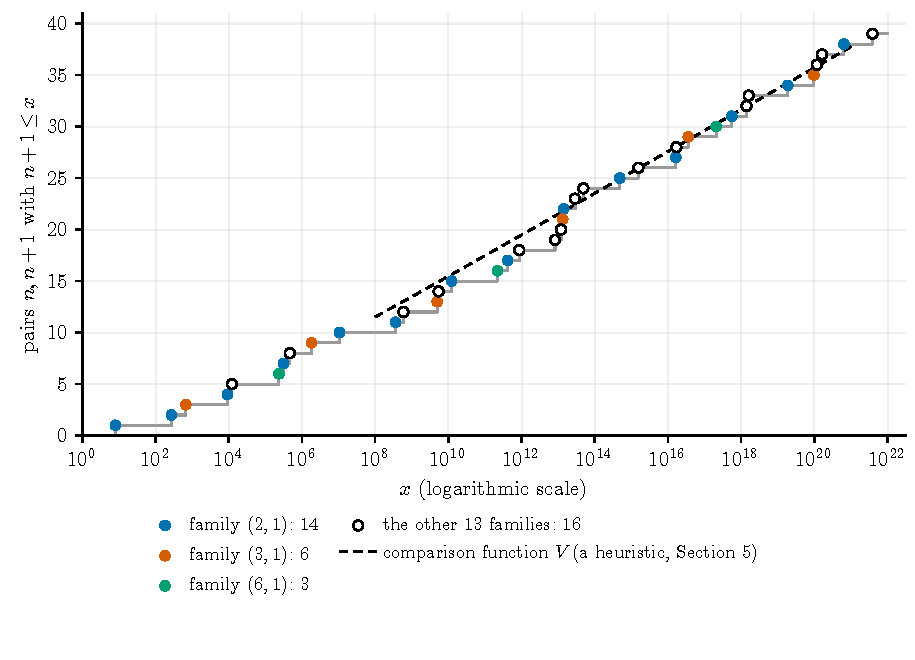
\includegraphics[width=\textwidth]{fig_treppe}
\caption{\textbf{The listed pairs up to $n_0$, and the family each comes from.} The \Z{fampaare} pairs $n, n + 1$ of powerful numbers with
$n \le n_0$ in the list of Proposition~\tref{prop:aufzaehlung}(b), which is complete below $2^{\Z{paare52exp}}$, as a staircase: each step is one pair, and each point is
colored by the family of Section~\tref{sec:familien} that contains it; the families with at least three pairs have their own color. The
positions come from the family formulas of Proposition~\tref{prop:perioden}, and at every power of ten from $10^8$ to $10^{21}$ the
staircase has exactly the number of pairs of our count, of which Table~\ref{tab:modell} shows every second one. The dashed line is the
comparison function of Section~\tref{sec:modell}, a heuristic yardstick, drawn from $10^8$ on, where that table begins.}\label{fig:treppe}
\end{figure}

A positive integer is \emph{powerful} if every prime that divides it divides it at least twice. There are infinitely many $n$ such that
$n$ and $n + 1$ are both powerful; the solutions of Pell equations give them, as Walker recounts \cite[p.~111]{Walker1976}. Erd\H{o}s asked
two further questions \cite{Bloom365}: whether all such pairs come from Pell equations, that is, whether $n$ or $n + 1$ must be a square,
and whether the number $N_1(x)$ of such $n$ with $n + 1 \le x$ is bounded by a power of $\log x$. The first question has a negative answer:
Golomb's pair $12167, 12168$ has no square, and Walker showed that its family is infinite \cite[p.~111]{Walker1976}; Walker also described all
pairs through Pell equations \cite[Sections~2 and~3]{Walker1976}. The second question is open. The best upper bound we know is $N_1(x) \ll x^{29/100 + \epsilon}$,
from a preprint of Reuss \cite[Theorem~4]{Reuss2014}, after $x^{2/5}(\log x)^2$ and $x^{7/19}\log x$ by Chan
\cite[Theorems~3 and~4]{Chan2012} and $x^{\gamma}$ for every $\gamma > 61/180$ by Blomer and Sch{\"o}bel \cite[Theorem~3]{BlomerSchoebel2013}, all three for every fixed distance;
Tao \cite[Corollary~2.11]{Tao2026} proves $x^{2/5 + o(1)}$ for pairs at every fixed distance and discusses the question. The pairs at distance
two, $n - 1$ and $n + 1$ powerful, are the objects of Part~I, where their middles $n$ carry the question of three consecutive powerful
numbers; a question of Golomb about two consecutive odd powerful numbers was answered by Sentance \cite[p.~272]{Sentance1981}.

This part collects what we can prove, compute and measure about the count of pairs, at distance one and at distance two. It establishes an explicit
lower bound of the order $\log x$, with a computed constant, checks the known list of pairs, and places the counting problem for distance two in the kernels that
divide their own $U_1$, of which only \Z{reinhartgerade} with $T_1$ even have been found below $5.325 \cdot 10^{13}$, and which contain the
case in which Tao's argument is weakest, under a squarefreeness assumption.

\paragraph{Main results.}
\begin{itemize}
\item \emph{An explicit lower bound} (Proposition~\tref{prop:csechs}): $\liminf N_1(x)/\log x \ge \Z{csechs}$, from the families of Walker
  with a square and squarefree part at most $\Z{csechsbmax}$, and from those without a square and $bd \le \Z{walkerdmax}$. That there are infinitely many pairs is classical; we did not find an
  explicit constant in the literature.
\item \emph{The count at distance two is a sum over towers} (Proposition~\tref{prop:turmsumme}), and so $P_2(10^h) \ge \Z{turmc}\,h -
  \Z{turmtuerme}$ for every $h$ (Corollary~\tref{cor:untergrenze}). In the box of kernels up to $\Z{kernschranke}$ and middles below
  $10^{\Z{hoehe}}$ the list of pairs at distance two is complete: \Z{zeugenpunkte} with middle divisible by four (Part~I) and \Z{kdpaare}
  with middle $\equiv 2 \pmod 4$ (Proposition~\tref{prop:klassedrei}).
\item \emph{Localization} (Proposition~\tref{prop:lokalisierung}): up to $O(N^{2/9})$, the pairs at distance two with middle at most $N$
  are exactly the first pairs of the kernels $m$ with $m \mid U_1(m)$, so every bound $E_3(N) \ll N^\theta$ on the number of these kernels
  gives $P_2(N) \ll N^{\max(2/9,\,\theta)}$. The case in which the argument of Tao is weakest lies among these kernels when the numbers $n_2$ and $m_2$ of Remark~\tref{rem:tao} are
  squarefree.
\item \emph{The families with a square overtake the comparison function} (Proposition~\tref{prop:transient}): the count of pairs with a square in
  the families with squarefree part up to $\Z{quadbmax}$ exceeds the comparison function of Section~\tref{sec:modell} for every
  $x \ge e^{1000}$, and at every row of the table from $10^{\Z{quadablog}}$ on. So the agreement of such a model with the counts up
  to $n_0$, which we also record, is a fact about that range and not a law.
\end{itemize}

\paragraph{How to read this part.} Every statement is followed by a paragraph \emph{In words} that says what it means with as few formulas as possible; a
reader who wants the results can read the statements and these paragraphs. A reader who wants to check can read the proofs, the paragraphs
\emph{The computation}, and the tables; every number we computed is generated from the data files of the deposit or from a cited constant,
and every numbered statement carries
a label that says whether it is proved, taken from the literature, computed, measured, a heuristic, or open (see the table at the end).
A statement that combines several kinds carries the label of the part that needs the most trust: a proof that uses our own computation is labeled computed, and a proof that uses a published result is labeled proved.
Table~\ref{tab:legende2} collects the notation.

\paragraph{Plan.} Section~\tref{sec:familien} recalls Walker's families and their periods. Section~\tref{sec:aufzaehlung} lists the pairs
up to $2^{\Z{paare52exp}}$ from our own enumeration and checks the published list beyond it inside the families. Section~\tref{sec:schranke}
establishes the lower bound. Section~\tref{sec:modell} sets up the comparison function, marks it as a heuristic, shows that the square families
overtake it, and states the convergence question. Section~\tref{sec:abstandzwei} treats the pairs at distance two: the second class of
middles, the tower sum, the lower bound, the localization and the growth question. Section~\tref{sec:abstandeins} puts the pairs at distance
one on one Pell equation per kernel and tests the third neighbor. Section~\tref{sec:fragen} collects the open questions.

\section{Pell families}\tlabel{sec:familien}

\subsection{Pairs as solutions of one equation}

As in Part~I, $\operatorname{sqfree}(N)$ is the product of the primes that divide $N$ to an odd power, so that
$N = \operatorname{sqfree}(N)\, r^2$ for a positive integer $r$.

\begin{lemma}[powerful numbers]\tlabel{lem:form}\belegart{proved}
A positive integer $n$ is powerful if and only if $n = bY^2$ with $b = \operatorname{sqfree}(n)$ and $b \mid Y$. This is the usual
description of powerful numbers, in the form used below.
\end{lemma}

\begin{proof}
Write $n = bY^2$ with $b = \operatorname{sqfree}(n)$. For a prime $p \mid b$ we have $v_p(n) = 1 + 2v_p(Y)$, which is at least $2$ exactly
when $p \mid Y$. For a prime $p \mid n$ with $p \nmid b$ we have $p \mid Y$ and $v_p(n) = 2v_p(Y) \ge 2$ in any case.
\end{proof}

\inwords Every number is its squarefree part times a square. The number is powerful exactly when the squarefree part divides the
root of the square part; for example $72 = 2 \cdot 6^2$ is powerful because $2 \mid 6$, and $12 = 3 \cdot 2^2$ is not because $3 \nmid 2$.

\begin{proposition}[Walker {\cite[Sections~2 and~3]{Walker1976}}]\tlabel{thm:bijektion}\belegart{literature}
Let $n$ and $n + 1$ be powerful, and put $b = \operatorname{sqfree}(n)$, $d = \operatorname{sqfree}(n + 1)$, $Y^2 = n/b$, $X^2 = (n+1)/d$.
Then
\[
  dX^2 - bY^2 = 1, \qquad b \mid Y, \qquad d \mid X .
\]
Conversely, every solution in positive integers of this equation with $b, d$ squarefree, $b \mid Y$ and $d \mid X$ comes from exactly one
such pair, namely $n = bY^2$.
\end{proposition}

\begin{proof}
The first part is Lemma~\tref{lem:form} applied to $n$ and to $n + 1$. Conversely, $bY^2$ and $dX^2$ are consecutive, and they are
powerful by Lemma~\tref{lem:form}, because $\operatorname{sqfree}(bY^2) = b$ and $\operatorname{sqfree}(dX^2) = d$ for squarefree
$b$ and $d$. The number $n$ determines $b$, $d$, $X$ and $Y$.
\end{proof}

\inwords A pair of consecutive powerful numbers is the same thing as a solution of $dX^2 - bY^2 = 1$ with two divisibility conditions.
Golomb \cite{Golomb1970} sorted the pairs into two types, as Walker recounts in his introduction \cite[p.~111]{Walker1976}, and Walker described both types through
equations of this shape.

We call the set of pairs with a given $(b, d)$ the \emph{family} $(b, d)$. The order matters: in the family $(b, d)$ the smaller number has
squarefree part $b$. As $X^2 - Y^2 = 1$ has no solution in positive integers, $b$ and $d$ are not both $1$. If $b = 1$ or $d = 1$, one of
the two numbers is a square (Walker's type~I); if $b, d \ge 2$, neither is (type~II). By Proposition~\tref{thm:bijektion} every pair lies in
exactly one family.

\subsection{The pairs inside one family}

For type~I with $d = 1$ the equation is Pell's equation $X^2 - bY^2 = 1$. We use the notation of Part~I with $m = b$: $\varepsilon_b =
T_1 + U_1\sqrt{b}$ is its fundamental solution, $\varepsilon_b^{\,k} = T_k + U_k\sqrt{b}$, and $b' = \prod_{p \mid b,\ p \nmid U_1} p$.

\begin{proposition}[Walker {\cite[Theorems 2.2, 2.5, 3.2 and 3.5]{Walker1976}}]\tlabel{prop:perioden}\belegart{literature}
\begin{enumerate}
\item[(i)] Let $b \ge 2$. The pairs of the family $(b, 1)$ are $n = bU_k^{\,2}$, $n + 1 = T_k^{\,2}$ for exactly the $k \ge 1$ with
  $b' \mid k$.
\item[(ii)] Let $d \ge 2$. The family $(1, d)$ needs a solution of $Y^2 - dX^2 = -1$. If there is none, or if $d$ is even, the family is
  empty. Otherwise let $\eta = y_0 + x_0\sqrt{d}$ be the fundamental solution, $\eta^k = Y_k + X_k\sqrt{d}$ for odd $k$, and
  $g = d/\gcd(d, x_0)$. The pairs are $n = Y_k^{\,2}$, $n + 1 = dX_k^{\,2}$ for exactly the odd multiples $k$ of $g$.
\item[(iii)] Let $b, d \ge 2$, and let $\alpha = x_0\sqrt{d} + y_0\sqrt{b}$ be the smallest solution of $dX^2 - bY^2 = 1$ if there is one.
  All solutions are $\alpha^{j} = X\sqrt{d} + Y\sqrt{b}$ with $j$ odd. If $d$ is even and $x_0$ is odd, or $b$ is even and $y_0$ is odd,
  the family is empty. Otherwise its pairs come from exactly the odd multiples $j$ of $\ell$, the product of the odd primes that divide
  $bd$ but not $x_0 y_0$.
\end{enumerate}
\end{proposition}

\begin{proof}
Part~(i) is Lemma~\partref{I}{lem:walker} for $m = b$: $b \mid U_k$ if and only if $b' \mid k$. Part~(ii) follows in the same way. For odd $k$
the binomial theorem gives $X_k = \sum_{i \text{ odd}} \binom{k}{i} y_0^{\,k-i} x_0^{\,i} d^{(i-1)/2} \equiv k\, y_0^{\,k-1} x_0 \pmod p$ for a
prime $p \mid d$, and $y_0^2 \equiv -1 \pmod p$, so $y_0$ is invertible modulo $p$. Hence $p \mid X_k$ if and only if $p \mid k x_0$. If $d$ is
even, then $y_0$ is odd, $dx_0^2 = y_0^2 + 1 \equiv 2 \pmod 8$, so $x_0$ is odd and no $X_k$ with $k$ odd is even. If $d$ is odd, $d \mid X_k$
if and only if $g \mid k$. Part~(iii) is Walker's Theorems 3.2 and 3.5; the description of all solutions as odd powers of $\alpha$ is his
Theorem~3.1, which he takes from \cite[Theorem~9]{Walker1967}.
\end{proof}

\inwords Inside one family the pairs come at regular steps. For the family $(b, 1)$ one takes every $b'$-th power of the Pell solution, for
$(1, d)$ every $2g$-th power starting at the $g$-th, and for type~II the same with $\ell$. We call $b'$, $g$ and $\ell$ the \emph{period} of
the family. Walker proved all three parts; the proof of (i) and (ii) above is short enough to give here.

For the computations we used our own forms of these statements and checked them: part~(i) against direct iteration modulo $b$ for all
\Z{periodepk} squarefree $b \le \Z{periodepkmax}$, and our residue class form of part~(iii) against direct iteration modulo $bd$ for all
\Z{walkerpk} solvable equations with $b, d \ge 2$ and $bd \le \Z{walkerpkmax}$; all agreed. For the families in
Table~\ref{tab:familien} we also computed $b'$, $g$ and $\ell$ from Walker's definitions and found the periods of our computation.

\inwords The formulas were not only cited: a computer followed the powers one by one and found the pairs exactly where the formulas for parts (i) and (iii) say.

\subsection{The families of the known pairs}

Each family grows geometrically. Here and below, $\log$ is the natural logarithm; Table~\ref{tab:familien} gives
$\log_{10}$ for readability. If $n_1$ is its first pair, the $j$-th is about $n_1 F^{\,j-1}$, where $\log F = 2b'\log\varepsilon_b$ for
the family $(b, 1)$, $\log F = 4g\log\eta$ for $(1, d)$, and $\log F = 4\ell\log\alpha$ for type~II. Throughout this part
$n_0 = \Z{paarletzt}$ is term number \Z{fampaare} of the list in Section~\tref{sec:aufzaehlung}, so
$n_0 \approx \Z{paargrenze}$.
Table~\ref{tab:familien} lists the families of the \Z{fampaare} pairs of that list with $n \le n_0$: \Z{famzahl} families,
\Z{famquadrat} pairs with a square and \Z{famohne} without. The first pairs of the families $(46, 1)$, $(6, 1)$, $(1, 5)$ and $(3, 7)$ are the four examples in Walker's paper
\cite[pp.~113 and~116]{Walker1976}.

\begin{table}[ht]
\centering
\begin{tabular}{crrrr}
\hline
family $(b, d)$ & period & $\log_{10} n_1$ & $\log_{10} F$ & pairs \\
\hline
\Z{famtab}
\hline
\end{tabular}
\caption{The families of the pairs $n, n+1$ of powerful numbers with $n \le n_0 \approx \Z{paargrenze}$, ordered by their first pair $n_1$. The
period is $b'$, $g$ or $\ell$ of Proposition~\tref{prop:perioden}; $F$ is the growth factor from one pair of the family to the next.
Each row is checked against three computations: the count in the list of pairs, the count predicted from the family, and, for type~II,
the pairs generated from the family and factored.}\label{tab:familien}
\end{table}

\inwords Most of the known pairs sit in a few families. The family $(2, 1)$, which starts with $8$ and $9$, alone has \Z{famtabzwei} of them,
because its growth factor is small. Most other families contribute a single pair so far.

\subsection{Notation and terms at a glance}\tlabel{sec:legende}

Table~\ref{tab:legende2} collects the symbols and words of this part, with the place where each is defined.

\begin{table}[tp]
\centering
\footnotesize
\begin{tabular}{p{3.0cm} p{7.6cm} l}
\hline
symbol or term & meaning & defined in \\
\hline
powerful & every prime factor occurs at least twice & Lemma~\tref{lem:form} \\
$\operatorname{sqfree}(N)$ & the product of the primes that divide $N$ to an odd power & \S\tref{sec:familien} \\
family $(b, d)$ & the pairs $n, n + 1$ with $\operatorname{sqfree}(n) = b$ and $\operatorname{sqfree}(n + 1) = d$ & \S\tref{sec:familien} \\
type I, type II & one of $n$, $n + 1$ is a square ($b = 1$ or $d = 1$); neither is ($b, d \ge 2$) & \S\tref{sec:familien} \\
$\varepsilon_b$, $T_k$, $U_k$, $b'$ & as in Part~I, with the kernel $m = b$ & Proposition~\tref{prop:perioden} \\
$\eta$, $g$ & the smallest solution $y_0 + x_0\sqrt{d}$ of $y^2 - dx^2 = -1$, and $g = d/\gcd(d, x_0)$ & Proposition~\tref{prop:perioden} \\
$\alpha$, $\ell$ & the smallest solution $x_0\sqrt{d} + y_0\sqrt{b}$ of $dX^2 - bY^2 = 1$, and the product of the odd primes of $bd$
  that do not divide $x_0 y_0$ & Proposition~\tref{prop:perioden} \\
period & $b'$, $g$ or $\ell$: the step between the powers that give pairs & Proposition~\tref{prop:perioden} \\
growth factor $F$ & the factor from one pair of a family to the next; $\log F = 2b'\log\varepsilon_b$, $4g\log\eta$ or $4\ell\log\alpha$
  & \S\tref{sec:familien} \\
$n_0$ & term number \Z{fampaare} of the list of Section~\tref{sec:aufzaehlung}; the range of Table~\ref{tab:familien} is $n \le n_0$
  & \S\tref{sec:familien} \\
$N_1(x)$ & the number of pairs with $n + 1 \le x$ & Proposition~\tref{prop:csechs} \\
pair at distance two, middle & powerful numbers $n - 1$, $n + 1$; the number $n$ between them & \S\tref{sec:abstandzwei} \\
kernel $m$, $m'$, lattice point & as in Part~I: $m = \operatorname{sqfree}(n^2 - 1)$, and $n = T_k(m)$ with $k$ an odd multiple of $m'$
  & Lemma~\partref{I}{lem:gerademitte} \\
$P_2(N)$, $P_2(N; M)$ & the number of middles $n \le N$, all of them or those with kernel at most $M$ & \S\tref{sec:abstandzwei} \\
discard criterion & a proved lower bound for $T_k(m)$ that removes a kernel before any $T_k$ is computed & Theorem~\partref{I}{thm:reduktion} \\
tower & the middles $T_k(m)$ of one kernel $m$ with $T_1(m)$ even, one for each odd multiple $k$ of $m'$ & \S\tref{sec:abstandzwei} \\
$w(m)$, $c_M$ & the rate $1/(2m'\log_{10}\varepsilon_m)$ of one tower in pairs per decimal digit, and the sum of these rates up to $M$
  & Proposition~\tref{prop:turmsumme} \\
$E_J(N)$ & the number of kernels with $m' < J$ and $T_1(m)$ even whose first middle is at most $N$ & Proposition~\tref{prop:lokalisierung} \\
index $m'$, wing (ii), rung & the product of the primes of $m$ that do not divide $U_1$; the kernels with $m \mid U_1$; one pair of a tower
  & Part~I \\
$v_p(N)$, $c_1$, $c_2$, $a_p$ & the exponent of $p$ in $N$; the constants of $Q(x)$; the proportion of $n$ with $v_p(n) = 1$
  & \S\tref{sec:modell} \\
$N_Q^{*}(L)$ & the count of the pairs with a square from the family periods, by the floor formula & Proposition~\tref{prop:transient} \\
$Q(x)$, $\rho(x)$ & the number of powerful numbers up to $x$, and the derivative of its two main terms & \S\tref{sec:modell} \\
$C$, $V(x)$ & the local correction factor and the comparison function, a heuristic yardstick & Definition~\tref{def:vergleich} \\
$N_Q(x)$, born & the pairs with a square in the families with $b, d \le \Z{quadbmax}$; a family is born at the logarithm of its first pair
  & Proposition~\tref{prop:transient} \\
$D$, $R$, third number & $D = \operatorname{sqfree}(a(a + 1))$, $a(a + 1) = DR^2$; the neighbor $a - 1$ or $a + 2$ that is not excluded by $2$
  & Proposition~\tref{prop:abstandeins} \\
\hline
\end{tabular}
\caption{Symbols and terms of Part II.}\label{tab:legende2}
\end{table}

\section{Enumeration}\tlabel{sec:aufzaehlung}

\begin{proposition}[the known pairs]\tlabel{prop:aufzaehlung}\belegart{computed}
\begin{enumerate}
\item[(a)] There are exactly \Z{paare52} pairs $n, n+1$ of powerful numbers with $n + 1 \le 2^{\Z{paare52exp}}$.
\item[(b)] Let $n_0$ be term number \Z{fampaare} of the b-file of OEIS A060355 \cite{OEISA060355}, computed by D.~Johnson, which lists
  such pairs by their smaller member $n$. The families of Section~\tref{sec:familien}, with a square and squarefree part at most
  $\Z{csechsbmax}$ or without a square and $bd \le \Z{walkerdmax}$, generate exactly \Z{fampaare} pairs with $n \le n_0$ from their
  fundamental solutions, each checked by complete factorization and by the identity $dX^2 - bY^2 = 1$ with $b \mid Y$ and $d \mid X$. The
  first \Z{paare52} of them are the pairs in (a), and the \Z{fampaare} pairs are exactly the first \Z{fampaare} terms of the b-file
  (Proposition~\tref{prop:quadratvollstaendig}). That no pair with $n \le n_0$ lies outside these families is a statement of that
  enumeration, not of ours.
\end{enumerate}
\end{proposition}

\begin{proof}[The computation]
(a) We listed all powerful numbers below $2^{\Z{paare52exp}}$ block by block, the block $k$ being $[2^k, 2^{k+1})$, each number written as
$a^2 b^3$ with $b$ squarefree; this form is unique. The size of every block agrees with the count $\sum_{b} \lfloor \sqrt{x/b^3} \rfloor$ over
squarefree $b$, taken at the two ends of the block. Inside a block the pairs are neighbors at distance one. A pair across two blocks would be
$(2^k - 1, 2^k)$, and $2^k - 1$ is not powerful for $2 \le k \le \Z{mersennemax}$, by complete factorization.
(b) The pairs are generated by the recursion of the Pell equation from the fundamental solution of each family, as in the proof of
Proposition~\tref{prop:quadratvollstaendig}; both members of every pair are factored completely, and the identity is checked with the
squarefree parts $b$ and $d$. The comparison with the b-file is made at run time against a copy that the reader supplies; the terms of the
b-file are not stored in the data deposit.
\end{proof}

\inwords Up to $2^{\Z{paare52exp}}$ we found all pairs ourselves. Beyond that we used a published list and
checked that each of its entries really is a pair; we did not check that the list misses nothing.

Mian and Siddique \cite{MianSiddique2026} describe the larger enumerations as exhaustive below $10^{22}$ but not certified. We rely on
it only where we say so. The next statement checks it inside the families of Section~\tref{sec:familien}, independently of the list.

\begin{proposition}[completeness inside the families]\tlabel{prop:quadratvollstaendig}\belegart{computed}
\begin{enumerate}
\item[(a)] In the families with a square, $(b, 1)$ and $(1, d)$ with $b, d \le \Z{quadratbmax}$, the pairs with $n \le n_0$ are exactly
  the \Z{famquadrat} pairs with a square among the terms of Proposition~\tref{prop:aufzaehlung}(b). They lie in \Z{famquadratfam} families.
\item[(b)] In the families without a square with $bd \le \Z{walkerdmax}$, the pairs with $n \le n_0$ are exactly the \Z{famohne} pairs
  without a square among those terms.
\end{enumerate}
\end{proposition}

\begin{proof}[The computation]
For every family in the range we generated its pairs from Proposition~\tref{prop:perioden} up to $n_0$ and compared them with the terms, in
both directions: no generated pair is missing from the terms, and no term with a square (in (a)) or without a square (in (b)) is missing
from the generated pairs. For (b) each generated pair was also factored completely, and both numbers are powerful.
\end{proof}

\inwords Every one of the \Z{fampaare} known pairs comes out of our own family computation, and within the families we searched our
computation finds no pair that the list lacks. So the list is complete for these families. Outside them, for example a family $(b, 1)$ with
$b > \Z{quadratbmax}$ whose first pair lies below $n_0$, a missing pair would not be noticed here.

\section{An explicit lower bound}\tlabel{sec:schranke}

\begin{proposition}[explicit lower bound]\tlabel{prop:csechs}\belegart{computed}
Let $N_1(x)$ count the pairs $n, n+1$ of powerful numbers with $n + 1 \le x$. Then
\[
  \liminf_{x\to\infty} \frac{N_1(x)}{\log x} \ge \Z{csechs} .
\]
The \Z{csechsfamq} nonempty families with a square and squarefree part at most $\Z{csechsbmax}$ contribute \Z{csechsquadrat}, and the
\Z{csechsfamw} nonempty families without a square and with $bd \le \Z{walkerdmax}$ contribute \Z{csechswalker}.
\end{proposition}

\begin{proof}
Let $F$ be the growth factor of a nonempty family, as in Section~\tref{sec:familien}. We first show that its $j$-th pair satisfies
$n_j + 1 \le F^{\,j}$. In the family $(b, 1)$ the $j$-th pair has $n_j + 1 = T_{jb'}^{\,2}$ by Proposition~\tref{prop:perioden}(i), and
$T_k = (\varepsilon_b^{\,k} + \varepsilon_b^{-k})/2 \le \varepsilon_b^{\,k}$, so $n_j + 1 \le \varepsilon_b^{\,2jb'} = F^{\,j}$. In the family
$(1, d)$ the $j$-th pair comes from $k = (2j - 1)g$, and for odd $k$ the conjugate of $\eta^k$ is $-\eta^{-k}$, so
$X_k\sqrt{d} = (\eta^k + \eta^{-k})/2 \le \eta^k$ and $n_j + 1 = dX_k^{\,2} \le \eta^{2(2j-1)g} \le \eta^{4jg} = F^{\,j}$. For type~II the $j$-th
pair comes from the exponent $(2j - 1)\ell$, the conjugate of $\alpha^i = X\sqrt{d} + Y\sqrt{b}$ is $X\sqrt{d} - Y\sqrt{b} = \alpha^{-i}$, and
the same computation gives $n_j + 1 = dX^2 \le \alpha^{4j\ell} = F^{\,j}$.

Hence a family has at least $\lfloor \log x / \log F \rfloor \ge \log x / \log F - 1$ pairs with $n + 1 \le x$. Different families have
different pairs by Proposition~\tref{thm:bijektion}. So for every finite set $S$ of nonempty families
\[
  N_1(x) \ge \sum_{f \in S} \Bigl( \frac{\log x}{\log F_f} - 1 \Bigr), \qquad
  \liminf_{x\to\infty} \frac{N_1(x)}{\log x} \ge \sum_{f \in S} \frac{1}{\log F_f} .
\]
For the two sets named in the statement we computed the sums; the total is rounded down.
\end{proof}

\inwords Each family on its own produces pairs at a steady rate on a logarithmic scale: the number of its pairs below $x$ grows like
$\log x$ divided by the logarithm of its growth factor. Since no pair belongs to two families, the rates add up. Adding them for all
families up to the stated sizes gives the constant. Families outside these ranges can only increase it.

\section{A heuristic comparison model, and the convergence question}\tlabel{sec:modell}

This section compares the count $N_1(x)$ of Section~\tref{sec:schranke} with a function that a simple probabilistic picture suggests. The
picture is a heuristic. We use the function only as a yardstick, and we do not claim that it predicts anything; the only statement of
this section that is not a heuristic is Proposition~\tref{prop:transient}, and the lower bound of Section~\tref{sec:schranke} does not depend on the picture.

\subsection{The comparison function}

Let $Q(x)$ be the number of powerful numbers up to $x$. Erd\H{o}s and Szekeres found the main term, and Bateman and Grosswald proved
$Q(x) = c_1 \sqrt{x} + c_2 x^{1/3} + O(x^{1/6})$ \cite{ErdosSzekeres1934}, \cite[Theorem~1]{BatemanGrosswald1958}, with $c_1 = \zeta(3/2)/\zeta(3)$ and $c_2 = \zeta(2/3)/\zeta(2)$, so that $c_2 < 0$. Let
$\rho(x) = c_1/(2\sqrt{x}) + c_2/(3x^{2/3})$ be the derivative of the two main terms.

\begin{definition}[comparison function; a heuristic]\tlabel{def:vergleich}\belegart{heuristic}
For a prime $p$ let $a_p = (p - 1)/p^2$, the proportion of integers $n$ with $v_p(n) = 1$, and let
\[
  C = \prod_{p} \frac{1 - 2a_p}{(1 - a_p)^2}, \qquad V(x) = C \int_8^x \rho(t)^2\, dt .
\]
\end{definition}

The picture behind $V$ is this. If ``$n$ is powerful'' and ``$n + 1$ is powerful'' were independent events of probability $\rho(n)$ each, the
expected number of pairs with $n + 1 \le x$ would be about $\int_8^x \rho(t)^2\, dt$, which grows like $(c_1^2/4) \log x = \Z{naivrate} \log x$.
The events are not independent: a prime $p$ cannot divide both $n$ and $n + 1$, so the events $v_p(n) = 1$ and $v_p(n + 1) = 1$ exclude
each other. Under the picture, the proportion of $n$ with $v_p(n) \ne 1$ and $v_p(n + 1) \ne 1$ is $1 - 2a_p$ instead of $(1 - a_p)^2$, and
the factor $C$ collects this correction over all primes, in the manner of the Hardy--Littlewood constants. Two assumptions enter here and
are not derived: that the primes act independently, and that these proportions, which are densities over all integers, may be applied to
powerful numbers; among powerful numbers the share of $n$ with $4 \mid n$ has a different limit (Remark~\partref{I}{rem:anteil}).
Numerically $C = \Z{modellc}$, so
$V(x)$ grows like $\Z{modellrate} \log x$. Heuristics with a local factor at each prime are used for related counting problems, for example
in \cite{vanDoorn2026}.

\inwords Powerful numbers get rarer as they grow, at a known rate. If two neighbors were powerful independently of each other, one could
compute how many pairs to expect. They are not independent, because a prime never divides two neighbors at once, and $C$ is one simple
correction for that, not a derived one. The result is a curve to compare with, not a prediction.

Table~\ref{tab:modell} sets $V$ against the count. Up to $n_0$ the list has \Z{modellnull} pairs; it is complete below $2^{\Z{paare52exp}}$
and inside the families of Proposition~\tref{prop:quadratvollstaendig}, and beyond that it is described as exhaustive but not certified
\cite{MianSiddique2026}. The comparison function gives \Z{modellnullkorr}, and the independent picture gives \Z{modellnullnaiv}. The
constant $C$ and the function $\rho$ contain nothing fitted to the data: we computed $V$ before we compared it with the terms beyond
$2^{\Z{paare52exp}}$, where the count is \Z{modellneu} against \Z{modellneukorr} for $V$ and \Z{modellneunaiv} for the independent picture.
The agreement is a fact about this range, within a scatter of about $\sqrt{N}$ for a count of $N$ pairs; beyond $2^{\Z{paare52exp}}$ the
comparison does not separate $V$ from the independent picture. The next statement shows that the agreement does not last.

\begin{table}[ht]
\centering
\small
\begin{tabular}{rrrr}
\hline
$\log_{10} x$ & pairs counted & $V(x)$ & independent picture \\
\hline
\Z{modelltab}
\hline
\end{tabular}
\caption{The number of pairs $n, n + 1$ with $n + 1 \le x$, the comparison function $V(x)$ of Definition~\tref{def:vergleich}, and the
uncorrected integral $\int_8^x \rho^2$. The counts up to $2^{\Z{paare52exp}}$ are our own enumeration; beyond it they come from the terms of
Proposition~\tref{prop:aufzaehlung}(b).}\label{tab:modell}
\end{table}

\subsection{The families with a square overtake the comparison function}

Let $N_Q(x)$ be the number of pairs $n, n + 1$ with $n + 1 \le x$ that lie in a family $(b, 1)$ or $(1, d)$ with $b, d \le \Z{quadbmax}$. By
Proposition~\tref{prop:perioden} these families are known exactly. For a family $f$ with first pair $n_1$ and growth factor $F$ put
$t_f = \log n_1$; we say the family is \emph{born} at $\log x = t_f$. By the formulas of Section~\tref{sec:familien}, $n_j + 1$ is
$(\alpha^{k} + \alpha^{-k})^2/4$ times a constant, with $\alpha$ the unit of the family and $k$ growing by the period from one pair to the
next; so $\log(n_j + 1) = \log(n_1 + 1) + (j - 1) \log F - \delta_j$ with $0 \le \delta_j < 2\log 2$, the correction coming from the
decreasing terms $\alpha^{-k}$. The count
\[
  N_Q^{*}(L) = \sum_{f} \max\Bigl(0,\ \Bigl\lfloor \frac{L - t_f}{\log F_f} \Bigr\rfloor + 1\Bigr),
\]
over the families with $b, d \le \Z{quadbmax}$, therefore agrees with $N_Q(e^L)$ except that a pair within $1/n_1$ of the boundary on the
logarithmic scale may fall on the wrong side.

\begin{proposition}[the families with a square overtake the comparison function]\tlabel{prop:transient}\belegart{computed}
\begin{enumerate}
\item[(a)] Table~\ref{tab:quad} gives $N_Q^{*}(L)$ and $V(e^L)$ for \Z{quadzeilen} values of $L = \log x$ up to $1000$. On a finer grid
  than the table, $N_Q^{*}$ first exceeds $V$ at $L = \Z{quadkreuz}$, that is, at $x \approx 10^{\Z{quadkreuzlog}}$; at the next row of the
  table it is below $V$ again, and from $L = \Z{quadab}$ on it is above $V$ at every row of the table.
\item[(b)] For every $L \ge 1000$, $N_Q(e^L) > V(e^L)$.
\end{enumerate}
\end{proposition}

\begin{table}[ht]
\centering
\small
\begin{tabular}{rrrrr}
\hline
$L = \log x$ & $N_Q^{*}(L)$ & $V(e^L)$ & independent picture & rate of the families born \\
\hline
\Z{quadtab}
\hline
\end{tabular}
\caption{The pairs with a square in the families with $b, d \le \Z{quadbmax}$, counted exactly from the family periods, against the
comparison function. The last column is $\sum 1/\log F$ over the families born by $L$, the rate at which $N_Q$ grows there.}\label{tab:quad}
\end{table}

\begin{proof}
(a) is the computation of the table. (b) Let $\mathcal{F}$ be the set of the \Z{quadgeboren} families with $b, d \le \Z{quadbmax}$ that are
born by $L = 1000$, and let $s = \sum_{f \in \mathcal{F}} 1/\log F_f = \Z{quadrate1000}$. Write $y_f(L) = (L - t_f)/\log F_f$. The $j$-th
pair of $f$ has $\log(n_j + 1) \le L$ as soon as $\log(n_1 + 1) + (j - 1) \log F_f \le L$, that is, $j \le (L - \log(n_1 + 1))/\log F_f + 1$; so
$f$ has more than $(L - \log(n_1 + 1))/\log F_f \ge y_f(L) - 1/(n_1 \log F_f)$ pairs with $n + 1 \le e^L$, and the last term is below $0.05$,
because $n_1 \ge 8$ and $\log F_f \ge 2 \log(2 + \sqrt 3) > 2.6$ for every family. On the other hand, each term of $N_Q^{*}(1000)$ is at most
$y_f(1000) + 1$. So for $L \ge 1000$,
\[
  N_Q(e^L) \;>\; \sum_{f \in \mathcal{F}} y_f(L) - 0.05\,|\mathcal{F}| \;\ge\; \bigl(N_Q^{*}(1000) - |\mathcal{F}|\bigr) - 0.05\,|\mathcal{F}|
  + s\,(L - 1000)\]
and $0.05\,|\mathcal{F}| < \Z{quadslack}$, so
\[
  N_Q(e^L) \;>\; \Z{quadrest1000} - \Z{quadslack} + s\,(L - 1000) .
\]
On the other side, $\frac{d}{dL} V(e^L) = C \rho(e^L)^2 e^L = C \bigl(c_1/2 + (c_2/3) e^{-L/6}\bigr)^2 < C c_1^2/4 = \Z{modellrate}$, because
$c_2 < 0$. Hence $V(e^L) \le V(e^{1000}) + \Z{modellrate}\,(L - 1000)$ with $V(e^{1000}) = \Z{quadv1000}$. Since $\Z{quadrest1000} - \Z{quadslack} >
\Z{quadv1000}$ and $s > \Z{modellrate}$, the claim follows. The value of $V(e^{1000})$ is rounded to one decimal and the product $C$ is
truncated; truncating $C$ increases $V$, and the margin is larger than the rounding, so both errors are on the safe side.
\end{proof}

\inwords The comparison curve grows at a fixed rate on a logarithmic scale. The families with a square alone grow faster once enough of
them have been born, and from $10^{\Z{quadablog}}$ on, at every row of the table, they produce more pairs than the curve gives for all pairs
together; for all $x \ge e^{1000}$ this is proved. So the curve matches the counts only in the range we can see, and it must fail beyond it.
It is a yardstick for the present, not a law.

\subsection{The convergence question}

By Proposition~\tref{prop:csechs}, $\liminf N_1(x)/\log x$ is at least the sum of $1/\log F$ over any finite set of families. The sum over the
families with a square and squarefree part at most $B$ is \Z{teilsumq1} for $B = 10$ and \Z{teilsumq2} for $B = 100$; Table~\ref{tab:teilsum} continues it and
adds the families without a square with $bd \le B$.

\begin{table}[ht]
\centering
\small
\begin{tabular}{rrrr}
\hline
$\log_{10} B$ & with a square, squarefree part $\le B$ & without a square, $bd \le B$ & sum \\
\hline
\Z{teilsumtab}
\hline
\end{tabular}
\caption{The partial sums $\sum 1/\log F$ over the families of Section~\tref{sec:familien}. The last entry of the last column is the constant
of Proposition~\tref{prop:csechs}.}\label{tab:teilsum}
\end{table}

\begin{question}[convergence of the rates]\tlabel{q:konvergenz}\belegart{open}
Does $\sum_f 1/\log F_f$, taken over all families, converge?
\end{question}

The increase per decade of $B$ shrinks in both columns of the table. We counted where the last increase comes from: in the decade
$10^5 < B \le 10^6$, families with $\log \varepsilon \le 100$ supply \Z{zuwq}\,\% of it among the families with a square and \Z{zuww}\,\%
among those without, and the largest one percent of the families supply \Z{zuwtopq}\,\% and \Z{zuwtopw}\,\%. So in the last decade we
computed, the increase is carried by a small share of the families, those with small units, not by many small contributions. Whether this
continues is not known.

A positive answer would not by itself give an asymptotic formula for $N_1(x)$. Families keep being born, and each newborn family adds a
pair at once; turning the sum of the rates into the rate of $N_1(x)$ needs control of how many families are born below every height, which we
do not have. The towers of Section~\tref{sec:abstandzwei} pose the same question for distance two, as Question~\tref{q:wachstum}.

This is also where an answer to the second question of Erd\H{o}s could come from. Every pair belongs to exactly one family, and a family has
about $\log x/\log F$ pairs below $x$. So $N_1(x)$ is governed by two quantities: how many families are born below $x$, and the sum of
their rates, which is Question~\tref{q:konvergenz}. If the number of families born below $x$ were bounded by a power of $\log x$, so would
be $N_1(x)$, and the answer to the question of Erd\H{o}s would be yes. We know no such bound, and no bound for the number of families
better than the upper bounds for $N_1(x)$ itself recalled in the introduction. We do not know whether it holds.

\inwords Every family contributes a rate, and the rates add up. Whether the total of all rates is finite is open. Our partial sums grow
more and more slowly, but they are driven by a small share of the families, those with small units, so a few more decades would not settle it.
Erd\H{o}s's question would be answered by showing that new families are born rarely enough; we cannot show this.

\section{Pairs at distance two}\tlabel{sec:abstandzwei}

A \emph{pair at distance two} is a pair $n - 1$, $n + 1$ of powerful numbers, and $n$ is its \emph{middle}. By
Lemma~\partref{I}{lem:gerademitte} the middle is even, and $n = T_k(m)$ for exactly one squarefree odd $m \ge 3$ with $T_1(m)$ even and one
odd multiple $k$ of $m'$. The kernel satisfies $m \equiv 7 \pmod 8$ when $4 \mid n$, and $m \equiv 3 \pmod 8$ when $n \equiv 2 \pmod 4$. We
write
\[
  P_2(N) = \#\{\, n \le N : n - 1 \text{ and } n + 1 \text{ are powerful} \,\},
\]
and $P_2(N; M)$ for the same count restricted to kernels $m \le M$. Proposition~\partref{I}{prop:paarliste} lists the middles divisible by
four in a box. The next statement does the same for the other middles, and the rest of the section counts both. Figure~\ref{fig:turmwald}
shows all these pairs at once.

\begin{figure}[t]
\centering
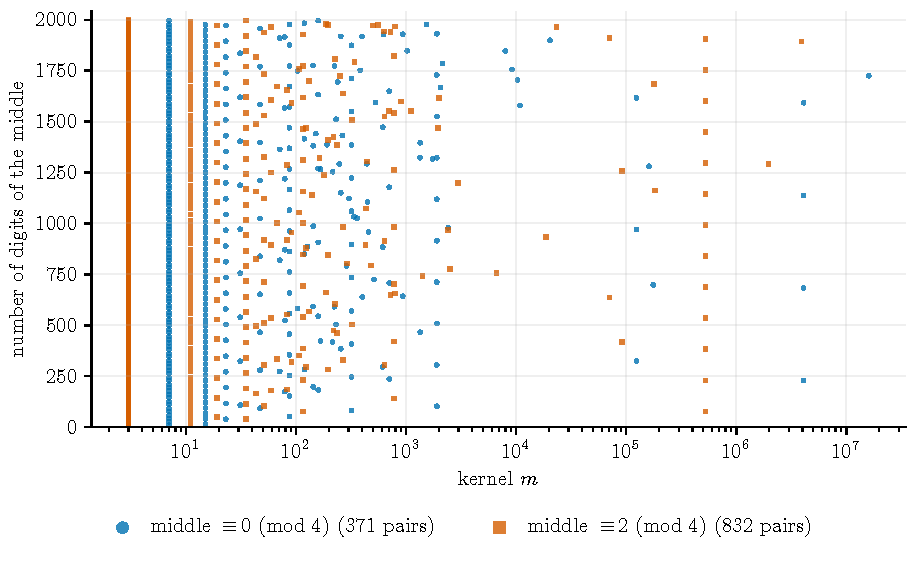
\includegraphics[width=\textwidth]{fig_turmwald}
\caption{\textbf{The pairs at distance two stand in towers.} The pairs at distance two with middle below $10^{\Z{hoehe}}$ and kernel at most $\Z{kernschranke}$, each placed at its kernel $m$
and the number of digits of its middle. The pairs of one kernel stand in a column at equal distances, the towers of
Proposition~\tref{prop:turmsumme}. The kernel $m = 3$ alone gives \Z{kddrei} of them. The column at $m = \Z{einkernm}$, with $m' = 3$, is
the kernel from the discussion of Question~\tref{q:wachstum}.}\label{fig:turmwald}
\end{figure}

\subsection{The middles that are not divisible by four}

\begin{proposition}[the middles that are not divisible by four]\tlabel{prop:klassedrei}\belegart{computed}
\begin{enumerate}
\item[(a)] Among the \Z{kdkerne} squarefree $m \equiv 3 \pmod 8$ with $m \le \Z{kdschranke}$, exactly \Z{kdkandidaten} pass the discard
  criterion of Theorem~\partref{I}{thm:reduktion} for the height $10^{\Z{hoehe}}$; the largest of them is $\Z{kdkernmax}$. Their lattice points
  $(m, k)$ with $T_k(m) < 10^{\Z{hoehe}}$ number \Z{kdpunkte}. For \Z{kdungerade} of them $T_1(m)$ is odd, and the other \Z{kdpaare} are
  exactly the middles $n \equiv 2 \pmod 4$ of pairs at distance two with $n < 10^{\Z{hoehe}}$ and $\operatorname{sqfree}(n^2 - 1) \le
  \Z{kdschranke}$.
\item[(b)] These \Z{kdpaare} middles have \Z{kdpaarkerne} different kernels, and the kernel $m = 3$ alone gives \Z{kddrei} of them.
\item[(c)] The list in (a) contains every middle $n \equiv 2 \pmod 4$ with $n < \Z{ohnetripelsicher}$, every such middle with
  $n < \Z{ohnetripel}$ if Reinhart's extended search missed nothing (Remark~\partref{I}{rem:reinhartliste}), and every such middle with
  $n < 10^{\Z{vollexpo}}/27$ whose kernel does not divide $U_1$.
\end{enumerate}
\end{proposition}

\begin{proof}
(a) is the computation of Theorem~\partref{I}{thm:reduktion}, run with the residue class $3$ in place of $7$, together with
Lemma~\partref{I}{lem:gerademitte}: a lattice point with $T_1$ odd has $T_k$ odd and gives no pair. (b) is a count in the list of (a).
(c) Let $n$ be such a middle and $m$ its kernel. Remark~\partref{I}{rem:siebenundzwanzig} gives the bound $T_k \ge (m^{3/2}/m')^{m'}$ in this
class too, so the proof of Corollary~\partref{I}{cor:kern} applies: if $m \nmid U_1$, then $m^{4.5}/27 < n$, and $m < \Z{kdschranke}$ for
$n < 10^{\Z{vollexpo}}/27$. If $m \mid U_1$, then $m^{3/2} < T_1(m) \le n$, so $n < \Z{ohnetripelsicher}$ forces $m < 1.5 \cdot 10^{12}$, the
range in which Reinhart's list of such kernels is complete \cite[Remark~5.5]{Reinhart2023}, and $n < \Z{ohnetripel}$ forces
$m < 5.325 \cdot 10^{13}$, the range of his extended search \cite{Reinhart2024}. The list has two kernels $m \equiv 3 \pmod 8$,
$1\,752\,299$ below the smaller bound and $20\,256\,129\,307\,923$ below the larger one. The first lies in the box of (a); its $T_1$ has
\Z{kdreinhartungst} digits and is odd. For the second, $T_1$ is even and has \Z{kdreinhartst} digits, so its first middle is far above
$\Z{ohnetripel}$.
\end{proof}

\inwords The middles of the form $4j + 2$ come from the kernels $m$ of the form $8j + 3$. In the box of kernels up to $\Z{kdschranke}$ and
middles below $10^{\Z{hoehe}}$ there are \Z{kdpaare} of them, and most come from a single kernel, $m = 3$. None of them is the middle of a
triple, since such a middle is divisible by $2$ exactly once.

\subsection{The count is a sum over towers}

For a kernel $m$ with $T_1(m)$ even, the middles $T_k(m)$ with $k$ an odd multiple of $m'$ form the \emph{tower} over $m$.

\begin{proposition}[the count is a sum over towers]\tlabel{prop:turmsumme}\belegart{proved}
For all integers $N, M \ge 1$,
\[
  P_2(N; M) \;=\; \sum_{\substack{3 \le m \le M \text{ odd, squarefree}\\ T_1(m) \text{ even}}}
  \#\bigl\{\, k \text{ an odd multiple of } m' : k \log \varepsilon_m \le \log (2N) \,\bigr\} .
\]
\end{proposition}

\begin{proof}
By Lemma~\partref{I}{lem:gerademitte} the middles $n \le N$ with kernel $m \le M$ correspond one to one to the pairs $(m, k)$ in the sum with
$T_k(m) \le N$. It remains to show that $T_k \le N$ exactly when $\varepsilon_m^{\,k} \le 2N$. We have $2T_k = \varepsilon_m^{\,k} +
\varepsilon_m^{-k}$ with $0 < \varepsilon_m^{-k} < 1$. If $T_k \le N$, then $\varepsilon_m^{\,k} < 2T_k \le 2N$. If $\varepsilon_m^{\,k} \le 2N$,
then $2T_k < 2N + 1$, and since $2T_k$ is an integer, $2T_k \le 2N$.
\end{proof}

\inwords Each kernel carries a tower of pairs, one on every rung $k$, and the rungs are evenly spaced on a logarithmic scale: from one rung to
the next the middle grows by the factor $\varepsilon_m^{\,2m'}$. Counting the pairs below a height is counting rungs below that height, tower by
tower.

We evaluated the right side for the kernels that pass the discard criterion in both classes and compared it with the lattice points that the
searches of Theorem~\partref{I}{thm:reduktion} and Proposition~\tref{prop:klassedrei} found. Table~\ref{tab:turm} shows six heights; the two
agree at every height in both classes. The last two columns are a negative control: the same count with the step $\log T_1$ in place of
$\log \varepsilon_m$, an error of an early version of our program, gives larger counts, which are wrong.

\begin{table}[ht]
\centering
\small
\begin{tabular}{rrrrr}
\hline
 & \multicolumn{2}{c}{pairs, counted and by the tower sum} & \multicolumn{2}{c}{negative control (step $\log T_1$)} \\
$h$ & middle $\equiv 0 \pmod 4$ & middle $\equiv 2 \pmod 4$ & middle $\equiv 0 \pmod 4$ & middle $\equiv 2 \pmod 4$ \\
\hline
\Z{turmtab}
\hline
\end{tabular}
\caption{Pairs at distance two with middle at most $10^h$ and kernel at most $\Z{kernschranke}$. The counted pairs and the tower sum of
Proposition~\tref{prop:turmsumme} agree in every row.}\label{tab:turm}
\end{table}

Each tower adds one pair every time $\log_{10} N$ grows by $2m' \log_{10} \varepsilon_m$. So $P_2(10^h; M)$ grows with $h$ at the average rate
\[
  c_M = \sum_{\substack{3 \le m \le M \text{ odd, squarefree}\\ T_1(m) \text{ even}}} w(m), \qquad w(m) = \frac{1}{2m' \log_{10} \varepsilon_m},
\]
pairs per decimal digit. For the towers of Table~\ref{tab:turm} the rate is \Z{turmc7} for the middles divisible by four and \Z{turmc3} for the
others. This rate belongs to the kernels up to $M$; it is not a rate for $P_2$ itself, because kernels above $M$ add towers of their own.
Whether $c_M$ stays bounded as $M$ grows is Question~\tref{q:wachstum}.

\begin{corollary}[lower bound at every height]\tlabel{cor:untergrenze}\belegart{computed}
For every integer $h \ge 1$,
\[
  P_2(10^h) \;\ge\; \Z{turmc}\, h - \Z{turmtuerme} .
\]
For the middles divisible by four alone, the count is at least $\Z{turmc7}\, h - \Z{turmtuerme7}$.
\end{corollary}

\begin{proof}
Take the \Z{turmtuerme} kernels $m \le \Z{kernschranke}$ with $T_1(m)$ even that pass the discard criterion, \Z{turmtuerme7} of them with
$m \equiv 7 \pmod 8$ and \Z{turmtuerme3} with $m \equiv 3 \pmod 8$. By Proposition~\tref{prop:turmsumme} the tower over $m$ has a pair with
middle at most $10^h$ for every odd $j$ with $j \le y_m$, where $y_m = (h + \log_{10} 2)/(m' \log_{10} \varepsilon_m)$. There are
$\lfloor (y_m + 1)/2 \rfloor > y_m/2 - 1/2$ such $j$, and $y_m/2 \ge h\, w(m)$. Different kernels give different middles. Summing over the
kernels gives more than $h \sum_m w(m) - \Z{turmtuerme}/2$ pairs. The sum of the weights is at least \Z{turmc}, and at least \Z{turmc7}
over the first class, which gives both bounds with half the subtracted constants; the statement keeps the larger ones.
\end{proof}

\inwords Every tower keeps producing pairs forever, one per rung. Adding up the rungs of the towers we know gives a lower bound for the number
of pairs below any height, however large. Any single tower already gives a bound of this shape; the constant here is the sum over the \Z{turmtuerme} towers
that pass the discard criterion. For heights below $10^{\Z{hoehe}}$ the count over these towers is exactly the number of pairs with kernel at most
$\Z{kernschranke}$, by Proposition~\tref{prop:turmsumme}.

That there are infinitely many pairs at distance two is classical \cite[p.~272]{Sentance1981}; Corollary~\tref{cor:untergrenze} only puts a number on
how fast they appear.

\subsection{Where the pairs live}

For an odd $J \ge 3$ let
\[
  E_J(N) = \#\{\, m \text{ odd, squarefree} : m' < J,\ T_1(m) \text{ even},\ T_{m'}(m) \le N \,\},
\]
the kernels whose first rung is a middle at most $N$ and whose index $m'$ is below $J$. For $J = 3$ these are the kernels with $m \mid U_1$ and
$T_1(m)$ even; those with $m \equiv 7 \pmod 8$ form wing~(ii) of Part~I (Corollary~\partref{I}{cor:fluegel}).

\begin{proposition}[localization of the pair count]\tlabel{prop:lokalisierung}\belegart{proved}
For every integer $N \ge 2$ and every odd $J \ge 3$,
\[
  P_2(N) \;\le\; 6J\,(J^J N)^{2/(3J)} + \frac{2}{\log 3}\,(J^J N)^{1/(3J)} \log N + \frac{2 \log N}{\log 3}\, E_J(N),
  \qquad E_J(N) \le P_2(N) .
\]
In particular $P_2(N) \le 18\,(27N)^{2/9} + \frac{2}{\log 3}(27N)^{1/9} \log N + \frac{2 \log N}{\log 3} E_3(N)$. Moreover,
\[
  E_3(N) \;\le\; P_2(N) \;\le\; E_3(N) + 41\, N^{2/9} + 3\, N^{1/9} \log N \;\le\; E_3(N) + 51\, N^{2/9} .
\]
\end{proposition}

\begin{proof}
By Lemma~\partref{I}{lem:gerademitte} every middle $n \le N$ is $T_k(m)$ for one kernel $m$ and one odd multiple $k$ of $m'$, with $T_1(m)$
even. For a fixed kernel, $T_k \ge T_1^{\,k}$ and $T_1 > \sqrt{m}$, so there are fewer than $2 \log N/\log m$ indices $k$ with $T_k \le N$.

Kernels with $m' \ge J$. By Remark~\partref{I}{rem:siebenundzwanzig}, $N \ge T_k \ge (m^{3/2}/m')^{m'}$. The function
$f(x) = x(1.5 \log m - \log x)$ increases on $[3, m]$ for $m \ge 8$, as in the proof of Corollary~\partref{I}{cor:kern}, and for $m = 7$ one
checks $f(3) < f(5) < f(7)$ directly; for $m = 3$ we have $m' = 3 = J$, and $m = 5$ does not occur, because $m \equiv 3$ or $7 \pmod 8$. So $N \ge (m^{3/2}/J)^J$, that is, $m \le M_J := (J^J N)^{2/(3J)}$. Using
$\sum_{3 \le m \le M} 1/\log m \le \sqrt{M}/\log 3 + 2M/\log M$ and $\log M_J \ge (2/(3J)) \log N$, these kernels contribute at most
\[
2 \log N\, \bigl(2M_J/\log M_J + \sqrt{M_J}/\log 3\bigr) \le 6J M_J + (2/\log 3) \sqrt{M_J} \log N
\]
middles.

Kernels with $m' < J$. Then $T_{m'}(m) \le T_k(m) \le N$, and $T_{m'}$ is even because $T_1$ is even and $m'$ is odd. So $m$ is counted by
$E_J(N)$, and it contributes fewer than $2 \log N/\log 3$ middles.

Finally, $m \mapsto T_{m'}(m)$ maps the kernels counted by $E_J(N)$ to different middles at most $N$; each $T_{m'}(m)$ is a middle
by the converse direction of Lemma~\partref{I}{lem:gerademitte}. So $E_J(N) \le P_2(N)$.

For the last statement take $J = 3$. The kernels with $m' \ge 3$ contribute at most $18(27N)^{2/9} + (2/\log 3)(27N)^{1/9} \log N$ middles,
as above. A kernel with $m' < 3$ has $m' = 1$, because $m'$ is odd, so $m \mid U_1$; its middles are the $T_k$ with $k$ odd, and the first of
them, $T_1$, is counted by $E_3(N)$. A second middle $T_k \le N$ with $k \ge 3$ requires $T_1^{\,3} \le T_3 \le N$. Since $m \mid U_1$, we
have $U_1 \ge m$ and $T_1^2 = 1 + m U_1^2 > m^3$, so $m < N^{2/9}$, and the number of odd $k \ge 3$ with $T_k \le N$ is at most
$\log N/(2 \log T_1) < \log N/(3 \log m)$. With the bound for $\sum 1/\log m$ above and $M = N^{2/9}$, these kernels contribute at most
$3 N^{2/9} + N^{1/9} \log N/(3 \log 3)$ further middles. Adding up, with $18 \cdot 27^{2/9} + 3 < 41$ and
$(2/\log 3)\, 27^{1/9} + 1/(3 \log 3) < 3$, gives the first bound, and $N^{1/9} \log N \le (9/e)\, N^{2/9}$ gives the second.
\end{proof}

\inwords There are two kinds of kernels. Those with a large index $m'$ must be small, because their towers start high; together they give only
at most of the order $N^{2/(3J)}$ pairs. All other pairs come from the kernels whose index is small, whose number is the open point, and each
of these gives only a logarithmic number of pairs. So the question of how many pairs there are is a question about how many kernels with
small index there are. A finer count shows that a kernel with $m \mid U_1$ almost always gives only its first pair: a second one needs
$T_1^{\,3} \le N$, which only kernels below $N^{2/9}$ can afford. So the pairs and these kernels agree up to $N^{2/9}$.

\begin{corollary}[what the localization says, and what it does not say]\tlabel{cor:lokalisierung}\belegart{proved}
\begin{enumerate}
\item[(a)] For every fixed odd $J \ge 3$, all but $O_J(N^{2/(3J)})$ of the middles counted by $P_2(N)$ have a kernel with $m' < J$.
\item[(b)] Since $E_J(N) \le P_2(N)$, Proposition~\tref{prop:lokalisierung} gives no bound for $P_2(N)$ by itself. Conversely, every bound
  $E_J(N) \ll N^\theta$ gives $P_2(N) \ll N^{\max(2/(3J),\, \theta)} \log N$. For $J = 3$ the factor $\log N$ is not needed: every bound
  $E_3(N) \ll N^\theta$ gives $P_2(N) \ll N^{\max(2/9,\, \theta)}$, and for $\theta \ge 2/9$ the two bounds are equivalent.
\end{enumerate}
\end{corollary}

\begin{proof}
Both parts are read off from Proposition~\tref{prop:lokalisierung}.
\end{proof}

\inwords The inequality moves the problem, it does not solve it: counting pairs is as hard as counting the kernels with small index, and for
those we have no better bound than the one for all pairs.

\begin{remark}[where Tao's argument is weakest]\tlabel{rem:tao}\belegart{proved}
For distance two, Chan \cite[Theorem~3]{Chan2012} proves $P_2(N) \ll N^{2/5} (\log N)^2$, Tao \cite[Corollary~2.11]{Tao2026} proves
$P_2(N) \ll N^{2/5 + o(1)}$ within a more general statement, and Blomer and Sch{\"o}bel \cite[Theorem~3]{BlomerSchoebel2013} prove
$P_2(N) \ll N^{\gamma}$ for every $\gamma > 61/180$, for every fixed nonzero difference. Tao \cite[Remark~2.12]{Tao2026} notes that his
argument is weakest when $n - 1 = n_1^2 n_2^3$ and $n + 1 = m_1^2 m_2^3$ with $n_1, n_2, m_1, m_2$ all of size about $N^{1/5}$. If moreover
$n_2$ and $m_2$ are squarefree, the kernel is $m = n_2 m_2$, of size about $N^{2/5}$. A kernel with $m \nmid U_1$ would give
$n > m^{4.5}/27$ by Corollary~\partref{I}{cor:kern} (with Remark~\partref{I}{rem:siebenundzwanzig} when $n \equiv 2 \pmod 4$), which exceeds $N$ for large $N$; so $m \mid U_1$, and $k = 1$, because $k \ge 3$ would give
$n \ge T_1^{\,3} > m^{9/2}$. Precisely, if $n \le N$ and $m \ge (27N)^{2/9}$, then $m \mid U_1(m)$ and $k = 1$. So, under the assumption that $n_2$ and $m_2$ are squarefree, the case in which Tao's argument is weakest lies in
the set counted by $E_3(N)$, the first rungs of kernels that divide $U_1$. We do not claim the converse: $E_3$ also counts kernels of other
sizes.
\end{remark}

\inwords The bounds cited above come from counting solutions of one equation. Tao says where his counting is weakest, and that place
lies inside the kernels of the localization when the numbers $n_2$ and $m_2$ are squarefree.

\subsection{How fast does the count grow?}

\begin{question}[growth of the tower rate]\tlabel{q:wachstum}\belegart{open}
Does $c_M = \sum_{m \le M} w(m)$, the sum over odd squarefree $m$ with $T_1(m)$ even of $w(m) = 1/(2m' \log_{10} \varepsilon_m)$, stay bounded as
$M \to \infty$?
\end{question}

The partial sums increase with $M$, so either they converge or they tend to infinity. We separate what is proved, what is measured and what is
heuristic.

\emph{Proved and computed.} Proposition~\tref{prop:turmsumme} writes $P_2(N; M)$ as an exact tower sum, and Corollary~\tref{cor:untergrenze} gives
$P_2(10^h) \ge \Z{turmc}\, h - \Z{turmtuerme}$. Neither answer to the question is excluded. An answer would not give an asymptotic formula for
$P_2(N)$ by itself: that also needs to know how many kernels have a tower that reaches below $N$, and this is governed by the same unknown
kernels.

\emph{Measured.} Table~\ref{tab:wachstum} gives $c_M$ for $M = 10, 10^2, \dots, \Z{wtabmax}$ in both classes. In both, the increase from one decade to
the next becomes smaller. Single kernels matter: in the second class the kernel $m = \Z{einkernm}$, with $m' = 3$, alone gives about
\Z{einkernanteil}\,\% of the increase from $M = 10^5$ to $M = 10^6$.

\begin{table}[ht]
\centering
\small
\begin{tabular}{rrr}
\hline
$\log_{10} M$ & $c_M$, $m \equiv 7 \pmod 8$ & $c_M$, $m \equiv 3 \pmod 8$ \\
\hline
\Z{wtab}
\hline
\end{tabular}
\caption{The partial sums $c_M$ of Question~\tref{q:wachstum}, over all kernels up to $M$ with $T_1(m)$ even, without a height limit.}
\label{tab:wachstum}
\end{table}

\emph{Heuristic, not a claim.} The quotient $m/m'$ is the product of the primes of $m$ that divide $U_1$. A simple model says that a
prime $p \mid m$ divides $U_1$ with probability $1/p$. For the kernels up to $\Z{wtabmax}$ with $T_1$ even and the primes $p \le \Z{modellp}$, the
measured frequency divided by $1/p$ lies between \Z{modell7min} and \Z{modell7max} in the first class and between \Z{modell3min} and
\Z{modell3max} in the second; $m' = m$ holds for \Z{beins7}\,\% and \Z{beins3}\,\% of the kernels. Under the model, with independence over
the primes of $m$, and if $\log \varepsilon_m$ is of the order $\sqrt m$, the expected contribution of a kernel to $c_M$ is about
$m^{-3/2 + o(1)}$, and the expected sum converges. The model is checked only for $p \le \Z{modellp}$, and $\log \varepsilon_m$ is far below
$\sqrt m$ in families such as $m = t^2 - 2$ (Remark~\partref{I}{rem:designa}). The sum could still diverge through kernels with a small
index $m'$; whether they
occur often enough is exactly what the question asks. The example above shows why more decades of the same computation would say little: a
single such kernel can supply a large part of a decade.

\inwords Every kernel adds a small amount to the rate at which pairs appear. The question is whether these amounts add up to a finite total.
Our numbers grow more and more slowly, which is compatible with a finite total and equally with a slowly growing one; one kernel with a
small index can change the picture, so the data do not decide it.

\section{Distance one along the Pell route}\tlabel{sec:abstandeins}

Section~\tref{sec:familien} describes a pair $a, a + 1$ by the two squarefree parts $b$ and $d$. This section uses their product instead. That
puts every pair on the equation $x^2 - Dy^2 = 1$ for one kernel $D$, as Part~I does for the middles at distance two, and it makes the
question of Part~I easy to ask: a triple is a pair whose third neighbor is powerful as well.

\begin{proposition}[pairs on one Pell equation]\tlabel{prop:abstandeins}\belegart{proved}
Let $a \ge 1$, $T = 2a + 1$ and $D = \operatorname{sqfree}(a(a + 1))$, and write $a(a + 1) = D R^2$. Then $T^2 - D(2R)^2 = 1$, and $a$ and
$a + 1$ are both powerful if and only if $D \mid R$.
\end{proposition}

\begin{proof}
We have $T^2 - 1 = 4a(a + 1) = 4DR^2$. Since $a$ and $a + 1$ are coprime, every prime factor of $a(a + 1)$ divides exactly one of them, with
the same exponent; so both are powerful if and only if $a(a + 1)$ is. By Lemma~\tref{lem:form}, $a(a + 1) = DR^2$ is powerful if and only if
$D \mid R$.
\end{proof}

\inwords Two neighbors are both powerful exactly when their product is. The product is a squarefree number $D$ times a square $R^2$, and it is
powerful exactly when $D$ divides $R$. So the pairs with a given $D$ are found among the solutions of one Pell equation.

For a family $(b, d)$ of Section~\tref{sec:familien} one has $D = bd$ and $R = XY$, so Proposition~\tref{prop:abstandeins} is
Proposition~\tref{thm:bijektion} written with one kernel instead of two. The solutions of $x^2 - Dy^2 = 1$ with $x$ odd carry these pairs; the
solutions with $x$ even carry the middles at distance two of Lemma~\partref{I}{lem:gerademitte}. A triple of consecutive powerful numbers is a
pair $a, a + 1$ for which $a - 1$ or $a + 2$ is powerful as well, and one of the two is excluded at once: the even member of the pair is
powerful, hence divisible by $4$, so its neighbor at distance two is $2$ more than a multiple of $4$ and not powerful. We call the other one
the \emph{third number} of the pair.

\begin{proposition}[the third number]\tlabel{prop:abstandeinsrechnung}\belegart{computed}
\begin{enumerate}
\item[(a)] For the \Z{a1kerne} squarefree $D \le \Z{a1dmax}$, the pairs $a, a + 1$ of Proposition~\tref{prop:abstandeins} with
  $2a + 1 < 10^{\Z{a1hoehe}}$ number \Z{a1paareh}. The program ran each kernel one rung further, which adds the next pair above this
  bound for \Z{a1ueber} kernels; together these are the \Z{a1paare} pairs of (b) and (c). A direct search for consecutive powerful numbers
  up to $\Z{a1nmax}$, which does not use the equation, finds \Z{a1paare25} pairs, and the route with $D \le \Z{a1dmax25}$ finds the same
  \Z{a1paare25}.
\item[(b)] For \Z{a1zeuge1} of these pairs the third number has a prime factor $p < \Z{a1p1}$ with exponent $1$, and for \Z{a1zeuge2}
  more a prime factor $p < \Z{a1p2}$ with exponent $1$. For the remaining \Z{a1rest2}, all prime factors below $\Z{a1p2}$ occur at least
  twice. After removing them, the rest of the third number is a prime in \Z{a1s2prim} cases, \Z{a1s2primzert} of them proved by a deterministic test \cite{SorensonWebster2017} and the other
  \Z{a1s2ecpp}, with up to \Z{a1s2ecppmax} digits, by elliptic curve certificates \cite{GoldwasserKilian1986,AtkinMorain1993} that PARI/GP \cite{PARI2172}
  produced and a separate program of ours checked; in \Z{a1s2ecm} further cases the elliptic curve method finds a prime factor with exponent $1$.
\item[(c)] So for all but \Z{a1s2offen} of the \Z{a1paare} pairs a prime with exponent $1$ is known for the third number, and it is proved prime. For the \Z{a1s2offen} others no witness is known; the
  smallest of their third numbers has \Z{a1s2kleinst} digits.
\end{enumerate}
\end{proposition}

\begin{proof}[The computation]
(a) For each $D$ we solved $x^2 - Dy^2 = 1$, took the powers $T_k + U_k\sqrt{D}$ with $T_k$ odd below $10^{\Z{a1hoehe}}$, and kept those with
$D \mid U_k$ and $T_k \equiv \pm 1 \pmod 8$. For odd $D$ the second condition follows from the first; for $D = 2D_0$ the two together say
$2D_0 \mid U_k/2$. In both cases they are equivalent to $D \mid U_k/2 = R$, so by Proposition~\tref{prop:abstandeins} these are exactly the
pairs. The comparison in (a) was made up to $\Z{a1nmax}$ with a
separate program that lists all powerful numbers. (b) The third number is $a - 1 = (T - 3)/2$ or $a + 2 = (T + 3)/2$. For an odd prime $p$,
the exponent of $p$ in it is the exponent of $p$ in $T \mp 3$, which we computed from $T_k$ modulo $p^2$. For the remaining pairs we computed
the third number exactly, divided out all primes below $\Z{a1p2}$ and tested the rest; a prime rest divides the number exactly once. As
controls, the program finds for \Z{a1s2nk} pairs of the first group the prime found there, and for the pair with $(D, k) = (3, 24)$ it finds that
the third number $a - 1$ is itself a prime.
\end{proof}

\inwords For every pair we tried to show that its third neighbor is not powerful, by finding a prime that divides it only once. This worked
for all but \Z{a1s2offen} pairs. For those, we could not decide it; that does not make them triples. A triple among them with $2a + 1 < 10^{\Z{a1hoehe}}$ would also have to
avoid Part~I: its middle is below $10^{\Z{a1hoehe}}$, so by Theorem~\partref{I}{thm:reduktion} its kernel in the sense of Part~I would
exceed $\Z{kernschranke}$.

\section{Open questions}\tlabel{sec:fragen}

The problems left open in this part are the following. Each is stated where it arises; we collect them here.

\begin{enumerate}
\item[(1)] Erd\H{o}s asked whether the number $N_1(x)$ of pairs $n, n + 1$ of powerful numbers with $n + 1 \le x$ is bounded by a power of
  $\log x$ \cite{Bloom365}. Proposition~\tref{prop:csechs} gives $N_1(x) \gg \log x$ with an explicit constant; nothing in this part bounds $N_1(x)$
  from above.
\item[(2)] Question~\tref{q:konvergenz}: does the sum of $1/\log F$ over all families converge?
\item[(3)] Question~\tref{q:wachstum}: does the rate $c_M$ of the towers at distance two stay bounded?
\item[(4)] The question below, which Corollary~\tref{cor:lokalisierung} and Remark~\tref{rem:tao} single out.
\end{enumerate}

\begin{question}[the kernels that divide $U_1$]\tlabel{q:ezwei}\belegart{open}
Is there a $\theta < 61/180$ with $E_3(N) \ll N^{\theta}$? Since $E_3(N) \le P_2(N)$, Blomer and Sch{\"o}bel give $E_3(N) \ll N^{\gamma}$
for every $\gamma > 61/180$ \cite[Theorem~3]{BlomerSchoebel2013}; the question is whether the squarefree odd $m$ with $m \mid U_1(m)$,
$T_1(m)$ even and $T_1(m) \le N$ are rarer than that.
\end{question}

By Corollary~\tref{cor:lokalisierung}(b), a positive answer gives $P_2(N) \ll N^{\max(2/9,\, \theta)}$, and for $\theta \ge 2/9$ it is
equivalent to that bound. Either way it would improve the best exponent we know for distance two. Reuss's exponent $29/100$ is for distance one \cite[Theorem~4]{Reuss2014}, and for
distance two the best exponent we know is the $61/180$ of Blomer and Sch{\"o}bel. Remark~\tref{rem:tao} shows that the case in which Tao's
argument is weakest lies in $E_3$ when $n_2$ and $m_2$ are squarefree. What is known is small: the known kernels counted by $E_3$ are the members of Reinhart's list with $T_1(m)$ even. Their number below $1.5 \cdot 10^{12}$ is
\Z{reinhartgeradesicher} \cite[Remark~5.5]{Reinhart2023}, and below $5.325 \cdot 10^{13}$ it is \Z{reinhartgerade} on his extended list
\cite{Reinhart2024}, if that list is complete (Remark~\partref{I}{rem:reinhartliste}); each of them has
$T_1(m) > 10^{\Z{reinhartt1}}$ (Proposition~\partref{I}{prop:reinhart} for the class $7$, and \Z{kdreinhartst} digits for the kernel of class
$3$), and every other kernel has $T_1(m) > m^{3/2}$ by Corollary~\partref{I}{cor:kern}. So $E_3(N) = 0$ for
$N < \Z{ohnetripelsicher}$, and for $N < \Z{ohnetripel}$ under that assumption. A bound for $E_3$ is a statement about fundamental units, of
the kind that Part~I also needs in its wing~(ii).

\inwords Four questions remain. Two ask whether rates that we computed add up to a finite total. One is Erd\H{o}s's question itself. The
last asks how many kernels of the kind that divides $U_1$ there are; a positive answer would improve the best bound we know for pairs at distance
two, and it is the same gap that Part~I runs into.

\section*{The type of every statement}

Every statement of this part carries one of six labels, printed after its number. The table lists them; it is generated from the text by the build and checked against a second, independent reading of the source.

\input{../gemeinsam/belegtab_\teilnr}


\renewcommand{\teilnr}{III}\setcounter{section}{0}
\clearpage
\part*{Part III: further observations}\addcontentsline{toc}{part}{Part III: further observations}
%
%
%
%

\section*{Introduction}\addcontentsline{toc}{section}{Introduction}

Parts~I and~II study triples and pairs of consecutive powerful numbers. Along the way we measured and proved a number of things that sit at
the edge of these two questions and belong to neither. This part collects them. None of them is an attack on the questions of Erd\H{o}s,
and several are consequences or tests of published results; where that is so, the source is named at the statement.

\paragraph{What this part contains.} Section~\tref{sec:luecken} looks at the gaps between consecutive powerful numbers: the most frequent gap
values up to $10^{14}$ are powerful, although almost no gap value is, and an elementary lemma gives a mechanism that favors powerful gaps (Proposition~\tref{prop:kopf},
Remark~\tref{rem:decke}). Section~\tref{sec:zyklotomisch} treats powerful values of cyclotomic polynomials, which arise when a member of a
triple is a proper power: two explicit infinite chains, each giving powerful values of both $\Kreis{3}$ and $\Kreis{6}$ (Proposition~\tref{prop:phidrei}), a table up to
$\Z{zykschranke}$, and the case $x^4 + 1 = q^3 a^2$ (Proposition~\tref{prop:phiacht}). Section~\tref{sec:unabhaengig} tests the
independence assumption of Part~I along the divisors of the index, and states what the test can and cannot see. Section~\tref{sec:linsen}
measures the Wieferich fractions of Pell units, the quantity behind the rare events of Part~I, against the equidistribution that a
conjecture of Katz predicts. Section~\tref{sec:fragen} states two questions.

\paragraph{How to read this part.} Every statement is followed by a paragraph \emph{In words}. Every numbered statement carries a label that
says whether it is proved, taken from the literature, computed, measured, a heuristic, or open (see the table at the end); in this part most
statements are computations or measurements on a finite range, and they are stated as such. A statement that combines several kinds carries the label of the part that needs the most trust: a proof that uses our own computation is labeled computed, and a proof that uses a published result is labeled proved. Every number we computed is generated from the data files
of the deposit.

\begin{figure}[tp]
\centering
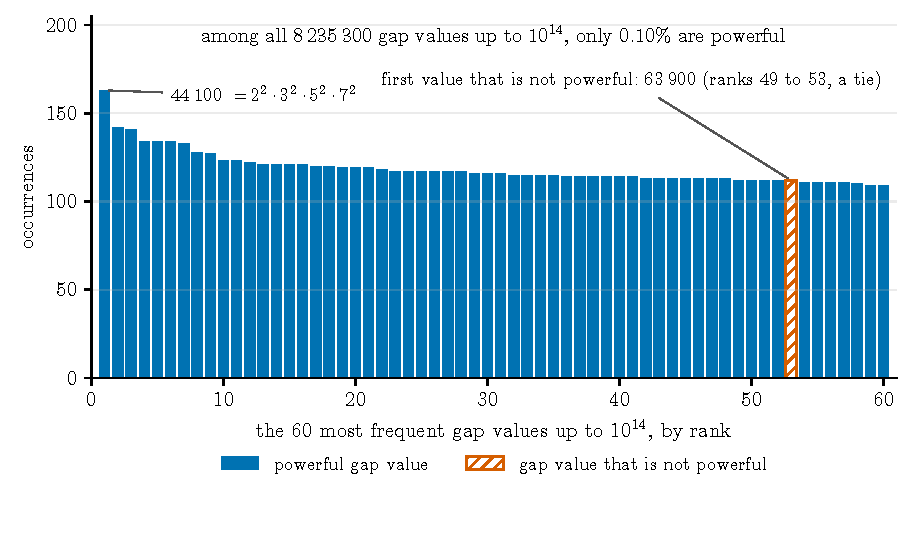
\includegraphics[width=\textwidth]{fig_luecken}
\caption{\textbf{Up to $10^{14}$, the \Z{lsbis} most frequent gap values are all powerful, although only \Z{lsanteil}\,\% of all gap values are.}
The sixty most frequent values of the gap between consecutive powerful numbers up to $10^{14}$, by their number of occurrences; values with
the same number share their rank and are ordered by size. The first \Z{lsbis} values are all powerful; the first
value that is not powerful, $\Z{lserster}$, shares its number of occurrences with powerful values (Proposition~\tref{prop:kopf}). Among all
\Z{lswerte} gap values up to $10^{14}$, only \Z{lsanteil}\,\% are powerful. The all-powerful head is shorter at $10^{14}$ than at $10^{12}$
(Table~\ref{tab:kopf}), so the picture says nothing about larger bounds (Question~\tref{q:luecken}).}\label{fig:luecken}
\end{figure}

\section{The gap spectrum of powerful numbers}\tlabel{sec:luecken}

Write the powerful numbers in increasing order and call the difference $g$ of two consecutive members a \emph{gap}; the sequence of gaps is
OEIS A076446 \cite{OEISA076446}. For an integer $g \ge 1$ let $\operatorname{sqfull}(g)$ be the product of the prime powers $p^{v_p(g)}$ with
$v_p(g) \ge 2$. Then $\operatorname{sqfull}(g) = g$ holds exactly when $g$ is powerful. Up to $10^{14}$ there are \Z{lsnpw} powerful numbers
and \Z{lswerte} distinct gap values, and only \Z{lsanteil}\,\% of these values are powerful; most of them are large and occur once. Among
the \Z{lsbasiswerte} values that occur at least \Z{lsbasismind} times, \Z{lsbasisanteil}\,\% are powerful. This section shows that the most
frequent gap values are nevertheless powerful, and gives a mechanism that favors them.

\begin{lemma}[Bajpai, Bennett and Chan {\cite[proof of Theorem~1.1]{BajpaiBennettChan2024}}]\tlabel{lem:ggt}\belegart{literature}
Let $n$ and $n + g$ be powerful. Then $\gcd(n, g)$ is powerful and divides $\operatorname{sqfull}(g)$. In particular $\gcd(n, g) = 1$ if $g$
is squarefree, and $g \mid n$ is possible only if $g$ is powerful.
\end{lemma}

\begin{proof}
If a prime $p$ divides $n$ and $g$, it divides $n + g$, so $p^2$ divides $n$ and $n + g$ and hence their difference $g$. So every prime of
$\gcd(n, g)$ occurs in it at least twice, and with an exponent at most $v_p(g)$, where $v_p(g) \ge 2$. If $g \mid n$, then
$\gcd(n, g) = g$ is powerful.
\end{proof}

That $\gcd(n, g)$ is powerful is used, for $k$-full numbers and without a separate proof, by Bajpai, Bennett and Chan immediately before
their equation~(4.2); the consequence for $\operatorname{sqfull}(g)$ is immediate, and it is what we use.

\inwords If two powerful numbers are a distance $g$ apart, every prime they share with $g$ appears in $g$ at least twice. So the part of
$g$ that such a pair can share is its powerful part; for a gap without square factors there is nothing to share.

\begin{proposition}[the head of the gap spectrum]\tlabel{prop:kopf}\belegart{computed}
Up to $10^{14}$ the \Z{lsbis} most frequent gap values are all powerful; they are the values that occur more than \Z{lsocc} times. The first
value that is not powerful is $\Z{lserster} = 2^2 \cdot 3^2 \cdot 5^2 \cdot 71$, with \Z{lsocc} occurrences, and it is the only one among
the \Z{lsg100} values that occur at least as often as the hundredth most frequent. Among the \Z{lsg200} values that occur at least as often as
the two hundredth, \Z{lsg200pw} are powerful. Table~\ref{tab:kopf} gives the same count at $10^{12}$ and $10^{13}$.
\end{proposition}

\begin{table}[ht]
\centering
\small
\setlength{\tabcolsep}{3pt}
\begin{tabular}{rrrrrrrr}
\hline
 & powerful & gap & \% of values & most & all powerful & first value & powerful near \\
bound & numbers & values & powerful & frequent & to rank & not powerful & rank $200$ \\
\hline
\Z{lstab}
\hline
\end{tabular}
\caption{The gap values between consecutive powerful numbers up to three bounds (Proposition~\tref{prop:kopf}). Values of equal frequency
share a rank; the column ``all powerful to rank'' counts the values that occur more often than the first value that is not powerful,
and the last column counts the powerful values among those that occur at least as often as the two hundredth most frequent.}
\label{tab:kopf}
\end{table}

If the $50$ most frequent values were drawn at random from all gap values up to $10^{14}$, about \Z{lserwartet} of them would be powerful,
and about \Z{lsbasiserw} if they were drawn from the values that occur at least \Z{lsbasismind} times.
The most frequent value at $10^{13}$ and $10^{14}$ is $\Z{lstop1} = 2^2 \cdot 3^2 \cdot 5^2 \cdot 7^2$.

\inwords Almost no gap value is powerful, but nearly all of the frequent ones are. From $10^{12}$ to $10^{14}$ the share of powerful values near
the top rises, while the first exception moves up the list; the effect does not simply grow or fade with the bound.

\begin{remark}[a ceiling for common divisors]\tlabel{rem:decke}\belegart{computed}
By Lemma~\tref{lem:ggt}, a pair at gap $g$ shares at most $\operatorname{sqfull}(g)$ with $g$, and only a powerful $g$ can share all of
itself. Table~\ref{tab:decke} lists the \Z{lsdeckeanz} values that are not powerful among the \Z{lsg200} values of
Proposition~\tref{prop:kopf}. Each has a small powerful part that is itself a frequent gap value; values of equal frequency share a rank, so
the rank is given as a range. The share of occurrences in which the pair shares the full ceiling is \Z{lsanteilpw}\,\% for the \Z{lsg20}
values that occur at least as often as the twentieth most frequent, and \Z{lsanteilnpw}\,\% for these \Z{lsdeckeanz}. So both sides are
consistent with one mechanism, a pair sharing the largest divisor that the lemma allows; only the size of that divisor differs.
\end{remark}

\begin{table}[ht]
\centering
\small
\begin{tabular}{rrrrr}
\hline
$g$ & $\operatorname{sqfull}(g)$ & rank of $\operatorname{sqfull}(g)$ & occurrences of $g$ & \% with $\gcd = \operatorname{sqfull}(g)$ \\
\hline
\Z{lsdecke}
\hline
\end{tabular}
\caption{The frequent gap values up to $10^{14}$ that are not powerful (Remark~\tref{rem:decke}): all values that are not powerful and
occur at least as often as the two hundredth most frequent.}\label{tab:decke}
\end{table}

\inwords About half of the pairs at gap $\Z{lserster}$ share the factor $900$ with the gap, and $\Z{lserster}$ occurs nearly as often as
$900$ itself. A powerful gap can share all of itself with a pair; this is one reason why the head of the spectrum is powerful, not a proof
that it must be.

\begin{remark}[a counting model, measured]\tlabel{rem:zaehlmodell}\belegart{measured}
Write $g = \operatorname{sqfull}(g) \cdot c$ with $c$ squarefree, and let $\operatorname{occ}(g)$ be the number of occurrences of $g$ up to
$10^{14}$. Over the \Z{zmn} gap values with at least \Z{zmmin} occurrences, which have \Z{zmkerne} distinct parts $\operatorname{sqfull}(g)$
and \Z{zmkof_n} distinct cofactors $c$, we fitted $\log \operatorname{occ}(g) = u(\operatorname{sqfull}(g)) + v(c)$ with one free value per
part and per cofactor. Evaluated on the values held back from the fit, in five random splits of about four fifths to one fifth over the gap
values, with the mean effect used for a part or cofactor that the fit has not seen and an affine recalibration fitted on the training part,
the model accounts for $\Z{zmr2} \pm \Z{zmr2sd}$ of the variance of $\operatorname{occ}(g)$ and $\Z{zmr2log} \pm \Z{zmr2logsd}$ of the
variance of $\log \operatorname{occ}(g)$, against $\Z{zmroh} \pm \Z{zmrohsd}$ for a regression of $\operatorname{occ}(g)$ on plain arithmetic
features of $g$ on the same values; the margin is positive in each split. The part alone accounts for \Z{zmkern}, the cofactor alone for
\Z{zmkof}, and on the fitted values the product $u \cdot v$ is uncorrelated with the residuals ($r = \Z{zmww}$). The values of $v$ are
reproducible up to a reliability of \Z{zmdecke}, which bounds what any explanation of $v$ can reach; on the \Z{zmdeutstufen} cofactors with
at least \Z{zmdeutkmin} gap values, the size and the prime factors of $c$ account for \Z{zmdeutung} of $v$ on held-back cofactors in one
split, against a ceiling of \Z{zmdeutdecke} measured on the same cofactors.
\end{remark}

The lemma therefore explains why the most frequent values can be powerful, not how often a value occurs: in this model the powerful part
alone accounts for \Z{zmkern} of the variance and the squarefree rest for \Z{zmkof}. This is a measurement on a finite range and not a
statement about all gaps. A version that splits $g$ over all its powerful divisors
instead of the canonical one fits the counts of the observed pairs $(g, \gcd)$ closely, but does not predict new gap values significantly better than the plain
arithmetic features ($\Z{zmallesep} \pm \Z{zmallesepsd}$ against $\Z{zmalleroh} \pm \Z{zmallerohsd}$), because about half of its cofactors
occur at a single gap; the record of this negative result is part of the deposit.

\inwords For the gap values that occur at least \Z{zmmin} times, knowing the powerful part and the squarefree rest of a gap predicts about half
of the variation in how often it occurs, and the rest matters more than the powerful part. The prediction was tested on gaps that the fit
had not seen. It describes the data up to $10^{14}$; it is not a law.

\begin{remark}[common factors of pairs]\tlabel{rem:primitiv}\belegart{measured}
In a sample of every \Z{pmschritt}th consecutive pair up to $10^{14}$, \Z{pmstich} pairs in total, the two members are coprime in
\Z{pmanteil}\,\% of the cases. The most frequent common divisors are \Z{pmgcd}, all powerful, as Lemma~\tref{lem:ggt} requires.
\end{remark}

\inwords About half of the neighboring pairs of powerful numbers share a factor, and the shared factor is always powerful.

We also computed the number variance of the powerful numbers in windows of up to \Z{nvlmax} mean spacings. It lies within about
\Z{nvrel}\,\% of a sum of independent lattice variances, and the large-window form of that sum grows like $L^{2/3}$ with the constant of
Chan's theorem \cite[Theorem~2]{Chan2026Variance}; in our windows the measured growth, a slope of \Z{nvsteig} on a logarithmic scale, has not
yet reached the exponent $2/3$. This is a check of Chan's theorem and not a new result.

\emph{Prior art and its reach.} Apart from the lemma, we found no work on the distribution of the gap values between powerful numbers.
We checked the work of Bajpai, Bennett and Chan in full, the OEIS entries A076446 and A001694, and records on Zenodo; the citing works of
Bajpai, Bennett and Chan were queried in two databases, which returned three and none. The reach of this search is set by these databases.

\section{Powerful values of cyclotomic polynomials}\tlabel{sec:zyklotomisch}

Remark~\partref{I}{rem:zyklotomisch} explains where these values come from. If a member of a triple is a proper power $x^r$ with $r \ge 2$,
its neighbors $x^r - 1$ and $x^r + 1$ are products of values $\Kreis{e}(x)$ and $\Kreis{e}(-x)$ of cyclotomic polynomials. Two such values
share only primes that divide $2r$, so a value that is coprime to the others must itself be powerful. This section records what we know
about powerful values $\Kreis{d}(x)$ at integers $x \ge 2$. For $d = 3$, $4$ and $6$ the polynomial is quadratic, and the question belongs to
the study of powerful values of quadratic polynomials by De Koninck, Doyon and Luca \cite{DeKoninckDoyonLuca2011}.

\begin{remark}[the values $x^2 + 1$]\tlabel{rem:xquadrat}\belegart{computed}
A powerful number that is not a square can be written as $a^2 b^3$ with $b > 1$ squarefree, so $x^2 + 1 = \Kreis{4}(x)$ is powerful exactly
when $x^2 - b^3 y^2 = -1$ has a solution for some squarefree $b > 1$; this is the form (1)--(2) of De Koninck, Doyon and Luca
\cite[p.~2]{DeKoninckDoyonLuca2011}, and their Table~1 gives the smallest case, $682^2 + 1 = 5^3 \cdot 61^2$ \cite[p.~8]{DeKoninckDoyonLuca2011}.
For each such $b$ the solutions form an infinite family, the odd powers of the smallest one. We solved the equation for all \Z{znaqg}
squarefree $b$ with $1 < b \le \Z{znab}$: it has a solution for \Z{znamit} of them. The list of OEIS A175155 \cite{OEISA175155} of the values
$x$ with $x^2 + 1 = a^2 b^3$ begins $682$, $1\,268\,860\,318$, $1\,459\,639\,851\,109\,444$.
\end{remark}

\inwords The number $x^2 + 1$ is powerful for infinitely many $x$, but such $x$ are very sparse: after $682$ the next value in the
list of OEIS A175155 is above a billion. Each of them comes from a Pell-type equation, and only some of these equations have solutions.

\begin{proposition}[two explicit chains of powerful values of $\Kreis{3}$ and $\Kreis{6}$]\tlabel{prop:phidrei}\belegart{proved}
Let the map $(y, m) \mapsto (127 y + 672 m,\ 24 y + 127 m)$ act on the starting points $(37, 7)$ (the first chain) and $(5, 1)$ (the
second chain), and let $(y_j, m_j)$ be the point after $j$ steps. In both chains $y_j^2 - 28 m_j^2 = -3$ and $y_j$ is odd for every $j$; $7 \mid m_j$ exactly when
$j \equiv 0 \pmod 7$ in the first chain and exactly when $j \equiv 6 \pmod 7$ in the second; and the two chains contain every solution of
$y^2 - 28 m^2 = -3$ with $y, m > 0$. For every $j$ with $7 \mid m_j$ the number $x = (y_j - 1)/2$ satisfies
$\Kreis{3}(x) = 343\,(m_j/7)^2$, which is powerful, and $\Kreis{6}(x + 1) = \Kreis{3}(x)$. In particular $\Kreis{3}(x)$ and $\Kreis{6}(x)$ are
powerful for infinitely many $x$.
\end{proposition}

\begin{proof}
Since $127^2 - 28 \cdot 24^2 = 1$, the map preserves $y^2 - 28m^2$, and $37^2 - 28 \cdot 7^2 = 5^2 - 28 \cdot 1^2 = -3$. It preserves the parity
of $y$, because $672$ is even and $127$ is odd. Modulo $7$ it fixes $y$, because $672 \equiv 0$ and $127 \equiv 1$, and it adds $24 y \equiv 3y$ to
$m$. In the first chain $y_0 \equiv 2$ and $m_0 \equiv 0 \pmod 7$, so $m_j \equiv 6j \pmod 7$, which vanishes exactly when $j \equiv 0 \pmod 7$; in
the second $y_0 \equiv 5$ and $m_0 = 1$, so $m_j \equiv 1 + 15j \equiv 1 + j \pmod 7$, which vanishes exactly when $j \equiv 6 \pmod 7$.
For the completeness, let $\alpha = y + z\sqrt 7$ with $y, z > 0$ and $y^2 - 7z^2 = -3$. Its conjugate is $-3/\alpha$, so $2y = \alpha - 3/\alpha > 0$
gives $\alpha > \sqrt 3$. Dividing by $\varepsilon = 8 + 3\sqrt 7$ keeps the norm, and keeps the quotient above $\sqrt 3$ as long as $\alpha > \sqrt 3\,\varepsilon$;
so $\alpha = \beta \varepsilon^n$ with $n \ge 0$ and $\sqrt 3 < \beta \le \sqrt 3\,\varepsilon$. For $\beta = y' + z'\sqrt 7$ this gives
$z' = (\beta + 3/\beta)/(2\sqrt 7) < \sqrt 3\,(\varepsilon + 1)/(2\sqrt 7) < 6$, and among $1 \le z' \le 5$ only $z' = 1$ and $z' = 2$ make $7z'^2 - 3$ a
square, so $\beta = 2 + \sqrt 7$ or $\beta = 5 + 2\sqrt 7$. Multiplying by $\varepsilon$ replaces $(y, z)$ by $(8y + 21z, 3y + 8z)$, which swaps the
parities of $y$ and $z$; so $z = 2m$ is even exactly for $(2 + \sqrt 7)\varepsilon^n$ with $n$ odd and for $(5 + 2\sqrt 7)\varepsilon^n$ with $n$ even. Since
$(2 + \sqrt 7)\varepsilon = 37 + 14\sqrt 7$ and $\varepsilon^2 = 127 + 48\sqrt 7$, these are the two chains, and multiplying by $\varepsilon^2$ is the map. Finally
$4\Kreis{3}(x) = (2x + 1)^2 + 3 = y_j^2 + 3 = 28 m_j^2$, so $\Kreis{3}(x) = 7 m_j^2$, and $\Kreis{6}(x + 1) = (x + 1)^2 - (x + 1) + 1 =
\Kreis{3}(x)$.
\end{proof}

In the first chain the first member is $x = 18$ with $\Kreis{3}(18) = 7^3$; the next three have \Z{phidreistellen} digits. The value $x = 18$ is the entry
$k = 3$, $n = 37$ of Table~1 of De Koninck, Doyon and Luca, since $37^2 + 3 = 4\,\Kreis{3}(18)$ \cite[p.~8]{DeKoninckDoyonLuca2011}, and
they observe that for a quadratic polynomial one powerful value of this kind gives infinitely many \cite[p.~7]{DeKoninckDoyonLuca2011}.
Their reduction on that page, applied to $\Kreis{3}$ with squarefree part $7$, leads in our normalization to the equation
$y^2 - 28m^2 = -3$ with $7 \mid m$. We did not find there the explicit recurrence, the two chains and their completeness, the parity of
$y_j$, the period $7$, or the transfer to $\Kreis{6}$. A direct search over all $m \le \Z{phidreibrute}$ finds no solution outside the two
chains, as the proposition says. The two chains are
disjoint: going forward from $(5, 1)$ the values of $y$ are $5, 1307, \dots$, going backward they are negative from $(-37, 7)$ on, so $(37, 7)$
is not on the second chain. The prime $x$ with $\Kreis{3}(x) = 7^3 a^2$ reported by Lavi \cite{Lavi2026}, which we know from the description of his record, is the
member $j = \Z{phidreilavij}$ of the second chain. Other squarefree parts give other powerful values: the second value for $d = 3$ in
Table~\ref{tab:zyk} comes from the equation $y^2 - 52 m^2 = -3$ with $13 \mid m$, that is, with $13$ in place of $7$.

\inwords The polynomials $x^2 + x + 1$ and $x^2 - x + 1$ take powerful values infinitely often. A Pell equation produces them one after
another, in two chains, and every seventh step of each chain gives one. The idea that one solution gives infinitely many is in the
literature; we did not find the explicit chains there.

\begin{proposition}[powerful values up to a bound]\tlabel{prop:zyktafel}\belegart{computed}
Among the \Z{zykn} pairs $(d, x)$ with $3 \le d \le 12$, $x \ge 2$ and $\Kreis{d}(x) \le \Z{zykschranke}$, exactly \Z{zyktreffer} give a
powerful value $\Kreis{d}(x)$. They are listed in Table~\ref{tab:zyk}.
\end{proposition}

\begin{table}[ht]
\centering
\small
\begin{tabular}{rrrl}
\hline
$d$ & $x$ & $\Kreis{d}(x)$ & factorization \\
\hline
\Z{zyktab}
\hline
\end{tabular}
\caption{The powerful values $\Kreis{d}(x)$ with $3 \le d \le 12$ and $\Kreis{d}(x) \le \Z{zykschranke}$ (Proposition~\tref{prop:zyktafel}).
The pairs for $d = 3$ and $d = 6$ are related by $\Kreis{6}(x + 1) = \Kreis{3}(x)$.}\label{tab:zyk}
\end{table}

\inwords Up to the bound, powerful cyclotomic values occur only for $d = 3, 4, 5$ and $6$, and only \Z{zyktreffer} times. The case $d = 5$ is
$3^4 + 3^3 + 3^2 + 3 + 1 = 121 = 11^2$, a square.

\begin{remark}[a class without squares]\tlabel{rem:granvilleklasse}\belegart{computed}
The numbers $x_n = (x^n - 1)/(x - 1)$ satisfy $x_{n+2} = (x + 1)\,x_{n+1} - x\,x_n$, a recurrence with $b = x + 1$ and $c = -x$ coprime and
$b^2 + 4c = (x - 1)^2 > 0$. If $x \equiv 2 \pmod 4$, then $c \equiv 2 \pmod 4$, and Granville's theorem \cite[Theorem~3]{Granville2012} gives, for every
$d \notin \{1, 2, 3, 6\}$, a primitive prime factor of $x_d$ that divides it to an odd power. Such a prime divides $\Kreis{d}(x)$ and no
$\Kreis{e}(x)$ with $e \mid d$, $e < d$, so $\Kreis{d}(x)$ is not a square. It can still be powerful, since an odd exponent can be $3$. We
checked the consequence: for $x \equiv 2 \pmod 4$, $d \in \{4, 5, 7, \dots, 12\}$ and $\Kreis{d}(x) \le \Z{zykklasse}$ no value is a
square, while outside the class the square $\Kreis{5}(3) = 11^2$ appears at once, and for these degrees it is the only square outside the
class up to $\Z{zykklasse}$. Inside the class, $\Kreis{4}(682) = 5^3 \cdot 61^2$ is powerful without being a square.
\end{remark}

\inwords For arguments of the form $4j + 2$, a theorem of Granville shows that the cyclotomic values are never squares, apart from four
small degrees. Our check up to $\Z{zykklasse}$ agrees with it, and the example $\Kreis{5}(3) = 121$ shows that the condition on the argument cannot simply be
dropped. The theorem says nothing about cubes, so it does not decide whether such a value can be powerful.

\begin{proposition}[the simplest case of $\Kreis{8}$]\tlabel{prop:phiacht}\belegart{proved}
There are no positive integers $x$ and $a$ and no prime $q < 2 \cdot 10^{11}$ with $x^4 + 1 = q^3 a^2$.
\end{proposition}

\begin{proof}
For $q = 2$ there is nothing to prove, since $x^4 + 1 \equiv 1$ or $2 \pmod{16}$ while $8a^2 \equiv 0$ or $8 \pmod{16}$. Let $q$ be odd and
write $x^4 + 1 = q\,y^2$ with $y = qa$. By Cohn \cite[p.~1347 and Theorem~1]{Cohn1997b}, a solution requires $q \equiv 1 \pmod 8$ and a
solution of $v^2 - q u^2 = -1$; if $\alpha = c + b\sqrt{q}$ is the smallest one, $u_n = (\alpha^n - \bar\alpha^n)/(2\sqrt q)$ and
$v_n = (\alpha^n + \bar\alpha^n)/2$, then $x^2 = v_A$ and $y = u_A$, where $A$ is the squarefree part of $c$. Expanding $\alpha^n$ gives $u_n \equiv n\,c^{n-1} b \pmod q$. Since
$c^2 \equiv -1 \pmod q$, the prime $q$ divides neither $c$ nor $A$, so $q \mid y = u_A$ forces $q \mid b$. For $q \equiv 1 \pmod 8$ the
fundamental unit $(t + w\sqrt q)/2$ of $\mathbb{Q}(\sqrt q)$ has $t$ and $w$ even, because $t^2 - q w^2 = \pm 4$ is impossible with $t$
and $w$ odd; so it lies in $\mathbb{Z}[\sqrt q]$, equals $\alpha$, and $b = w/2$. Hence a solution requires $q \mid w$. The conjecture of
Ankeny, Artin and Chowla says that this never happens, and it has been verified for all primes $q \equiv 1 \pmod 4$ below $10^{11}$
\cite{vanderPoortenteRieleWilliams2001} and between $10^{11}$ and $2 \cdot 10^{11}$ \cite{vanderPoortenteRieleWilliams2003}.
\end{proof}

We checked the last step independently for the \Z{achtq} primes $q \equiv 1 \pmod 8$ below $\Z{achtgrenze}$: in none of them does $q$
divide $b$. The proposition covers only the case in which the squarefree part of $x^4 + 1$ is a single prime. For small squarefree parts
the literature settles the question completely: Cohn solved $x^4 + 1 = D y^2$ for all squarefree $D < 10^5$, and apart from $D = x^4 + 1$
with $y = 1$ the only solution is $261^4 + 1 = 70\,258 \cdot 257^2$ \cite[abstract]{Cohn1997b}. If $x^4 + 1$ is powerful and $D$ is its
squarefree part, then $D \mid y$; neither case allows this, so the squarefree part of a powerful $x^4 + 1$ is at least $10^5$.

\inwords The number $x^4 + 1$ is the eighth cyclotomic value. If it were a cube of a prime times a square, a theorem of Cohn would force a
very special divisibility in the smallest solution of a Pell equation, and that divisibility is exactly what a well-tested conjecture
forbids; computer searches by others confirm it far enough to exclude all primes below $2 \cdot 10^{11}$.

\section{An independence test along the divisors of the index}\tlabel{sec:unabhaengig}

The heuristic of Part~I treats the event that a prime of rank $d$ divides $T_d(m)$ at least twice as a rare event of probability about
$1/p$, independent of other such events (Proposition~\partref{I}{prop:exponenten}). Part~I tests independence across the primes of one
kernel. A lattice point $(m, k)$ with many divisors carries one such event for each divisor $d$ of $k$, and the divisors are linked: $q d$ is
a multiple of $d$. This section tests whether the events at $d$ and at $q d$ are coupled.

\begin{remark}[no joint event along the divisors, and the power of the test]\tlabel{rem:unabhaengig}\belegart{measured}
For the \Z{ukerne} kernels with the most lattice points in the box of Theorem~\partref{I}{thm:reduktion}, we took each rank $d$ and its smallest prime $p$ of rank $d$ below $\Z{up}$, and set
the status of $d$ to $1$ if $p^2 \mid T_d(m)$ and to $0$ otherwise. We then formed all pairs $(d, qd)$ with $q \in \{3, 5, 7, 11, 13\}$ for
which both ranks have such a prime: \Z{upaare} pairs. The status is $1$ at $d$ alone in \Z{u10} pairs, at $qd$ alone in \Z{u01}, and at both
in \Z{u11}; independence predicts \Z{uerw} pairs with both. To see what this test could detect, we simulated a coupling in which the status
at $qd$ copies the status at $d$ with probability $\rho$, independently for each pair: for $\rho = 0.1$ one expects about \Z{ukopie} copied
pairs, and in at least \Z{utrenn}\,\% of \Z{usim} simulations at least one joint event appeared, against less than \Z{utrennnull}\,\% for
$\rho = 0$.
\end{remark}

\inwords If the rare event at one rank made the same event at a multiple rank more likely, pairs with the event at both ranks would appear.
There are none. The test is not blind: a coupling in which one time in ten the second event copies the first would almost always have shown
up, and one of half that strength would still have shown up in most runs. A much weaker coupling, or one that makes the second event less
likely, could not be seen with so few events, and the test uses only the smallest prime of each rank.

The test is formally a $\chi^2$ test on the table, but with fewer than one expected joint event the statistic only records whether a joint
event occurs; the simulation measures exactly that. One event at a rank $d$ enters a pair for each $q$ with $qd$ occupied, so the \Z{u10}
pairs come from fewer distinct events; the simulation copies pair by pair and therefore overstates the power against a coupling that acts
once per event. In the prior-art search for this part (arXiv, Zenodo, Google Scholar and OEIS, at the level of titles and abstracts) we found
no earlier test of independence along the divisors of the index.

\section{Wieferich fractions of Pell units}\tlabel{sec:linsen}

For a squarefree $m$ and a prime $p \nmid 2m$ let $e = \left(\frac{m}{p}\right)$ and write $\varepsilon_m^{\,p - e} = A + B\sqrt m$ modulo $p^2$.
Then $A \equiv 1$ and $B \equiv 0 \pmod p$, and we call $y_p = \bigl((B/p) \bmod p\bigr)/p \in [0, 1)$ the \emph{Wieferich fraction} of
$\varepsilon_m$ at $p$. It vanishes exactly when the order of $\varepsilon_m$ modulo $p^2$ equals its order modulo $p$; for a prime with a
rank this is the condition $p^2 \mid T_{\alpha_m(p)}(m)$ of Part~I. In Katz's language \cite{Katz2015}, $\varepsilon_m$ is a point on the torus
$x^2 - m y^2 = 1$, and $y_p$ is its Wieferich fraction for the framing whose Lie lattice is $\mathbb{Z}\sqrt m$, which Katz describes
\cite[Section~6]{Katz2015}. His Framed Wieferich Conjecture \cite[Conjecture~6.1]{Katz2015} predicts that such fractions are equidistributed.

\begin{remark}[no deviation from equidistribution, memory or coupling]\tlabel{rem:wieferichbrueche}\belegart{measured}
For the \Z{wf3kerne} kernels of Section~\tref{sec:unabhaengig} and all primes $p < \Z{wf3p}$ with $p \nmid 2mU_1$, that is, for \Z{wfn} pairs
$(m, p)$, we computed $y_p$.
\begin{enumerate}
\item[(a)] \emph{Near zero.} For six thresholds $t$ from $10^{-2}$ to $10^{-7}$ the number of $y_p < t$ agrees with the exact expectation for
  uniform $y_p$; the largest deviation is $\Z{wfzmax}$ standard deviations. For example, $y_p < 10^{-4}$ holds \Z{wft4b} times against
  \Z{wft4e} expected, and $y_p = 0$ holds \Z{wftreffer} times against $\sum 1/p = \Z{wferw}$. Only \Z{wfnullrang} of these zeros lie at primes that divide
  some $T_k(m)$, which happens exactly when the order of $\varepsilon_m$ modulo $p$ is divisible by $4$; they are the Wieferich events of
  Part~I on these kernels (Remark~\partref{I}{rem:wfdaten}), and the other zeros do not appear there. Split by the $2$-adic valuation of the order of
  $\varepsilon_m$ modulo $p$ (odd, $2 \bmod 4$, $0 \bmod 4$) and by $e$ into \Z{wfklanz} classes, the smallest $p$-value of a $\chi^2$ test
  of uniformity is \Z{wfklpmin}, or \Z{wfklbon} after the Bonferroni correction.
\item[(b)] \emph{Along the primes.} For each kernel, the correlation of $y_p$ with the fraction $j$ primes later, for $j = 1, \dots,
  \Z{wglags}$, gives \Z{wgtests} tests; \Z{wgueber} exceed $|z| = 2.576$ against about \Z{wgerw} expected, the largest is $\Z{wgzmax}$, with
  Bonferroni $p = \Z{wgpbon}$. A memory planted in test data, with $5$ percent of the values replaced by their predecessor, is found with
  $z = \Z{wgpk}$.
\item[(c)] \emph{Between kernels.} For the \Z{wkpaare} pairs of kernels, the correlation of their fractions at common primes has largest
  $|z| = \Z{wkzmax}$, with Bonferroni $p = \Z{wkpbon}$; a planted correlation of strength $0.02$ is found with $z = \Z{wkpk}$.
\end{enumerate}
\end{remark}

\inwords For every unit and every prime there is a number between $0$ and $1$ that measures how close the prime comes to being a
Wieferich prime for that unit. Over more than five million such numbers, on \Z{wf3kerne} units and the primes below $\Z{wf3p}$, our tests find no deviation from independent uniform random numbers: near zero,
from one prime to the next, and from one unit to another. Katz's conjecture predicts (a); applied to the product of two such tori it also
predicts (c); (b) goes beyond it. The only computation of Wieferich fractions that his paper mentions is one for elliptic curves, by
Bombieri, reported as compatible with the conjecture. Censuses of the zeros $y_p = 0$ exist for single units, for example Ryan's for
$1 + \sqrt 2$ up to $10^9$ \cite[Sections~2.1 and~5.1]{Ryan2026}; we did not find a test of the distribution of the fractions themselves,
near zero, along the primes or between units. A finite test cannot prove equidistribution; it shows no deviation at the sizes the controls
can detect.

\section{Questions}\tlabel{sec:fragen}

\begin{question}[the most frequent gap]\tlabel{q:luecken}\belegart{open}
Let $g(x)$ be the most frequent gap between consecutive powerful numbers up to $x$. Is $g(x)$ powerful for all large $x$, and does the share
of powerful values among the $N$ most frequent gaps up to $x$ tend to $1$ when $N$ is fixed and $x \to \infty$?
\end{question}

Proposition~\tref{prop:kopf} and Table~\ref{tab:kopf} are consistent with the first part at three bounds up to $10^{14}$. For the second
part they point both ways: the share of powerful values among the two hundred most frequent rises, while the leading block in which all
values are powerful shrinks. Lemma~\tref{lem:ggt} gives powerful gaps an advantage; it does not show that the advantage wins in the limit.

\inwords Is the most common distance between neighboring powerful numbers always itself powerful, however far one looks? Up to $10^{14}$ it
is, but the data do not show a clear trend for the values just below the top.

\begin{question}[powerful values of $x^4 + 1$]\tlabel{q:phiacht}\belegart{open}
Is $x^4 + 1$ powerful for some integer $x \ge 1$?
\end{question}

By Proposition~\tref{prop:phiacht} and the paragraph after it, the squarefree part of such a value is at least $10^5$, and it is not a prime
below $2 \cdot 10^{11}$. For $x^2 + 1$ the answer is yes (Remark~\tref{rem:xquadrat}).

\inwords Can the eighth cyclotomic value $x^4 + 1$ ever be powerful? The fourth one, $x^2 + 1$, can. For $x^4 + 1$ only special shapes are
excluded so far.

\begin{remark}[a conjecture on the most frequent gap]\tlabel{rem:champion}\belegart{heuristic}
We state a weak and a strong form for the most frequent gap $g(x)$ of Question~\tref{q:luecken}. \emph{Weak form:} $g(x)$ tends to infinity with $x$,
and $g(x)$ is powerful for all large $x$. \emph{Strong form:} for all large $x$, $g(x)$ is the square of a product of the first primes,
$(2 \cdot 3 \cdots p_r)^2$, with $r$ growing with $x$. The strong form implies the weak one; the weak one claims only what the data and
Lemma~\tref{lem:ggt} support directly, and the strong one also names the shape. Up to $10^{12}$ the most frequent value
is $900 = (2 \cdot 3 \cdot 5)^2$, and up to $10^{13}$ and $10^{14}$ it is $\Z{lstop1} = (2 \cdot 3 \cdot 5 \cdot 7)^2$ (Table~\ref{tab:kopf}).
The reason we expect it is Lemma~\tref{lem:ggt}: if $g = P^2$ with $P$ squarefree and $P^2 \mid n$, then $n = P^2 m$ and
$n + g = P^2 (m + 1)$, so the primes of $P$ already occur at least twice in both numbers, and only the other primes of $m$ and $m + 1$
must occur squared. A larger $P$ frees more primes but leaves fewer $m \le x/P^2$; the smallest primes free the most for the smallest
cost, and as $x$ grows the balance moves to a larger $P$. A balance of this kind is behind the conjecture of Odlyzko, Rubinstein and Wolf
that the most frequent gap between consecutive primes eventually runs through the products of the first primes, $30$, $210$, $2310$
\cite{OdlyzkoRubinsteinWolf1999}; we found no such statement for powerful numbers. Two values do not make a trend. The weak form fails if
$g(x)$ stays bounded, or if a value that is not powerful is the most frequent gap for arbitrarily large $x$. The strong form fails in
addition if a powerful value of another shape, such as $3600$ or $3528$, which follow $900$ and $44\,100$ closely in the counts, is the most
frequent gap for arbitrarily large $x$. Which of the two forms is right is open.
\end{remark}

\inwords We expect the most common distance between neighboring powerful numbers to keep growing and to stay powerful (weak form), and
we suspect that it is always the square of $2 \cdot 3 \cdot 5 \cdots$, as $900$ and $44\,100$ are (strong form). For the primes a similar pattern is conjectured, with $30$, $210$, $2310$. This
is an expectation supported by two values and a mechanism, not a result.

\section*{The type of every statement}

Every statement of this part carries one of six labels, printed after its number. The table lists them; it is generated from the
text by the build and checked against a second, independent reading of the source.

\input{../gemeinsam/belegtab_\teilnr}


%
%
%
%
%
\section*{Data and code availability}\addcontentsline{toc}{section}{Data and code availability}

Every number of this \ifimband volume\else part\fi\ that we computed is generated from a result file of a data deposit or from a cited constant; no computed number is
typed by hand. The data deposit is archived with the collected volume, DOI \href{https://doi.org/10.5281/zenodo.23127547}{10.5281/zenodo.23127547}.

\paragraph{What the deposit contains.} The deposit has two parts. The core holds what the text cites: (i) the result files, in JSON and
plain text, behind every computed number, together with the raw output of the scripts that wrote them; (ii) the scripts, written in Python,
each stating before it runs what it expects to find and the positive and negative controls that it runs; (iii) a manifest with the SHA-256 hash
and the size of every file, which the build checks before it reads a result file; (iv) the decimal expansions of the building blocks of
Part~I that the searches left open (Proposition~\partref{I}{prop:raenge}), including those that the algebraic split of
Remark~\partref{I}{rem:zweiprimitive} settles; (v) the certificates and the second routes for the computations that settle a building block; and
(vi) the file \texttt{OPEN\_PROBLEMS.md}, which lists the open problems of the volume. The archive holds the remaining scripts and results of the
investigation, including negative results that the text does not print.

\paragraph{Where the files are.} The collected volume and its three parts are published as four linked records on Zenodo, and the same files
are in one repository on GitHub. The record of the collected volume (DOI \href{https://doi.org/10.5281/zenodo.23127547}{10.5281/zenodo.23127547}) holds the volume and the whole deposit,
the core and the archive described above. The record of each part holds that part and the result files that its text cites, and links to the
record of the volume. The repository (\href{https://github.com/berkay-yueksel-sayim/erdos-364-365-powerful-numbers-pell}{github.com/berkay-yueksel-sayim/erdos-364-365-powerful-numbers-pell}) holds the four PDFs and the deposit, and its README lists the four records. The records of Parts~I, II and~III have the DOIs \href{https://doi.org/10.5281/zenodo.23127703}{10.5281/zenodo.23127703}, \href{https://doi.org/10.5281/zenodo.23127705}{10.5281/zenodo.23127705} and~\href{https://doi.org/10.5281/zenodo.23127707}{10.5281/zenodo.23127707}.

\paragraph{How the numbers get into the text.} The source of the text refers to each computed number by a key. A build tool reads the result
file named for the key, verifies it against the manifest, computes the number in its printed form, and writes it into the text; it stops if a key
has no source or if a file differs from the manifest. The same tool generates the table of the types of the statements and the list of open
problems from the source of the text, and it is part of the core.

\paragraph{Software.} The scripts use Python~3.12 with gmpy2~2.3, SymPy~1.14 and NumPy~2.4. The elliptic curve method and its relatives are run
with GMP-ECM~7.0.6 \cite{GMPECM706}, used as an installed program inside a container image built from the Debian package and not part of the
deposit; the recipe of the image is in the core. The elliptic curve certificates for primality were produced in the same way with
PARI/GP~2.17.2 \cite{PARI2172} and are part of the deposit; a separate program of ours checks each of them, so the result does not
depend on that program. Further work is planned to support these certificates with a second prover written independently by us. The
text is set with pdf\TeX.

\paragraph{Licenses.} The text and the data are licensed under the Creative Commons Attribution 4.0 International License (CC BY 4.0), and
the code under the Apache License, Version 2.0. Programs of others that the scripts use as tools, such as GMP-ECM, are not part of the
deposit and keep their own licenses.

%
%
%
%
%
%
%
%
%
\section*{Use of AI tools}\addcontentsline{toc}{section}{Use of AI tools}

Generative AI tools were used throughout this work: large language models of the Claude family by Anthropic, mainly Claude Opus~5 and~5.5,
and also Claude Fable~5.1 and Claude Sonnet~5.5 and~5, between August and October 2026,
through the Claude Code environment. They were used to draft the text and the mathematical arguments, to write the computer programs, to
run and check the computations, and to search for and read the literature. The author works independently, is not trained as a number
theorist, and learned the subject actively during the work; the tools made it possible to carry out and check computations on this scale. The author led the work in stages: each stage was
set by a prompt that stated what it should achieve, within a stage the tools followed a plan agreed with the author, and the author considered
the results before giving the next prompt, revising the plan when the results required it. The author contributed ideas where they helped and
framed how a problem should be attacked, decided which statements to keep, and is responsible for the content. The programs of the project,
including its own checking and build tools, were developed with the AI tools, and the author started the long computations, such as the
factor searches, on the author's own machine.

Several parts of the checking do not rest on these tools. The elliptic curve primality certificates were produced by PARI/GP~2.17.2 and are
verified by a separate program, and the factor searches use GMP-ECM~7.0.6. Every computed number is generated by a program from deposited
data or from a cited constant, and the programs carry positive and negative controls. Proofs, numbers and citations were also checked in
independent passes by further instances of the AI tools that were given no access to the drafting context. These tools are not authors.


\bibliographystyle{amsplain}
\bibliography{../gemeinsam/literatur}
\end{document}
